% This LaTeX document needs to be compiled with XeLaTeX.
\documentclass[10pt]{article}
\usepackage[utf8]{inputenc}
\usepackage{graphicx}
\usepackage[export]{adjustbox}
\graphicspath{ {./images/} }
\usepackage{hyperref}
\hypersetup{colorlinks=true, linkcolor=blue, filecolor=magenta, urlcolor=cyan,}
\urlstyle{same}
\usepackage{amsmath}
\usepackage{amsfonts}
\usepackage{amssymb}
\usepackage[version=4]{mhchem}
\usepackage{stmaryrd}
\usepackage[fallback]{xeCJK}
\usepackage{polyglossia}
\usepackage{fontspec}
\usepackage{newunicodechar}
\setCJKmainfont{Noto Serif CJK JP}

\setmainlanguage{english}
\setmainfont{CMU Serif}

\title{组合趣题 }

\author{}
\date{}


%New command to display footnote whose markers will always be hidden
\let\svthefootnote\thefootnote
\newcommand\blfootnotetext[1]{%
  \let\thefootnote\relax\footnote{#1}%
  \addtocounter{footnote}{-1}%
  \let\thefootnote\svthefootnote%
}

%Overriding the \footnotetext command to hide the marker if its value is `0`
\let\svfootnotetext\footnotetext
\renewcommand\footnotetext[2][?]{%
  \if\relax#1\relax%
    \ifnum\value{footnote}=0\blfootnotetext{#2}\else\svfootnotetext{#2}\fi%
  \else%
    \if?#1\ifnum\value{footnote}=0\blfootnotetext{#2}\else\svfootnotetext{#2}\fi%
    \else\svfootnotetext[#1]{#2}\fi%
  \fi
}

\newunicodechar{×}{\ifmmode\times\else{$\times$}\fi}

\begin{document}
\maketitle
数学奥林匹克小丛书\\
咢二版

\section{初中卷}
\begin{center}

\includegraphics[max width=\textwidth]{2024_10_09_bce9f07034ef55fc9c97g-01}
\end{center}

周建新 编著

\section{图书在版编目(CIP)数据}
数学奥林匹克小丛书. 初中卷. 组合趣题/周建新编著.\\
-2 版.一上海: 华东师范大学出版社, 2012.1\\
ISBN 978 - 7 - 5617 - 9238 - 4\\
I. (1)数… II. (1)周… III. (1)中学数学课一初中一教学

参考资料 IV. (1)G634.603\\
中国版本图书馆 CIP 数据核字(2012)第007513号

数学奥林匹克小丛书(第二版)・初中卷\\
组合趣题(第二版)

\begin{center}
\begin{tabular}{|c|c|}
\hline
者 & 周建新 \\
\hline
总策划 & 倪 明 \\
\hline
项目编辑 & 孔令志 \\
\hline
审读编辑 & 陈信渏 \\
\hline
帧设计 & 高 山 \\
\hline
责任发行 & 郑海 \\
\hline
\end{tabular}
\end{center}

出版发行 华东师范大学出版社\\
社 址 上海市中山北路 3663 号 邮编 200062\\
网 址 www. ecnupress. \href{http://com.cn}{com.cn}\\
电 话 021-60821666 行政传真 021-62572105\\
客服电话 021-62865537 门市(邮购)电话 021-62869887\\
地 址 上海市中山北路 3663 号华东师范大学校内先锋路口\\
网 店 \href{http://hdsdcbs.tmall}{http://hdsdcbs.tmall}. com\\
印 刷 者 常熟文化印刷有限公司\\
开 本 $787 \times 109216$ 开\\
插 页 1\\
印张 5.5\\
字 数 95 千字\\
版 次 2012 年 7 月第二版\\
印 次 2012 年 7 月第一次\\
印 数 1—11000\\
书 号 ISBN 978-7-5617-9238-4/G・5526\\
定 价 13.00 元\\
出版人朱杰人\\
(如发现本版图书有印订质量问题, 请寄回本社客服中心调换或电话 021 - 62865537联系)

\section{总}
数学竞赛像其他竞赛活动一样,是青少年学生的一种智力竞赛。在类似的以基础科学为竞赛内容的智力竞赛活动中,数学竞赛的历史最悠久、国际性强,影响也最大。我国于1956年开始举行数学竞赛,当时最有威望的著名数学家华罗庚、苏步青、江泽涵等都积极参加领导和组织竞赛活动,并组织出版了一系列青少年数学读物,激励了一大批青年学生立志从事科学事业。我国于1986年起参加国际数学奥林匹克,多次获得团体总分第一,并于1990年在北京成功地举办了第 31 届国际数学奥林匹克,这标志着我国数学竞赛水平在国际上居领先地位,为各国科学家与教育家所瞩目。

我国数学竞赛活动表明,凡是开展好的地区和单位,都能大大激发学生的学习数学的兴趣,有利于培养创造性思维,提高学生的学习效率。这项竞赛活动,将健康的竞争机制引进数学教学过程中,有利于选拔人才。由数学竞赛选拔的优胜者,既有踏实广泛的数学基础,又有刻苦钻研、科学的学习方法,其中的不少青年学生将来会成为出色的科学工作者。在美国,数学竞赛的优胜者中后来成名如米尔诺(J. W. Milnor)、芒福德(D. B. Mumford)、奎伦 (D. Quillen)等都是菲尔兹数学奖的获得者;在波兰,著名数论专家辛哲尔 (A. Schinzel)学生时代是一位数学竞赛优胜者;在匈牙利,著名数学家费叶尔 (L. Fejér)、里斯(M. Riesz)、舍贵(G. Szegö)、哈尔(A. Haar)、拉多 (T. Radó)等都曾是数学竞赛获奖者。匈牙利是开展数学竞赛活动最早的国家,产生了同它的人口不成比例的许多大数学家!

在开展数学竞赛的活动同时,各学校能加强联系,彼此交流数学教学经验,从这种意义上来说,数学竞赛可能成为数学课程改革的"催化剂",成为培养优秀人才的有力措施。

不过,应当注意在数学竞赛活动中,注意普及与提高相结合,而且要以普及为主,使竞赛具有广泛的群众基础,否则难以持久。

当然,现在有些人过于关注数学竞赛的成绩,组织和参与都具有很强的功利目的,过分扩大数学竞赛的作用,这些都是不正确的,违背了开展数学竞赛活动的本意. 这些缺点有其深层次的社会原因,需要逐步加以克服,不必因\\
$\qquad$

为有某些缺点, 就否定这项活动。\\
我十分高兴看到这套《数学奥林匹克小丛书》的正式出版. 这套书, 规模大、专题细. 据我所知, 这样的丛书还不多见. 这套书不仅对数学竞赛中出现的常用方法作了阐述, 而且对竞赛题作了精到的分析解答, 不少出自作者自己的研究所得,是一套很好的数学竞赛专题教程,也是中小学生和教师的参考书.

这套小丛书的作者都是数学竞赛教学和研究人员,不少是国家集训队的教练和国家队的领队. 他们为我国开展数学竞赛的活动和我国学生在 IMO 上取得成绩、为国争光作出了贡献, 为这套书尽早面世付出了艰辛的劳动。 华东师大出版社在出版《奥数教程》和《走向 IMO》等竞赛图书基础上,策划组织了这套丛书,花了不少心血。我非常感谢作者们和编辑们在这方面所做的工作,并衷心祝愿我国的数学竞赛活动开展得越来越好。\\
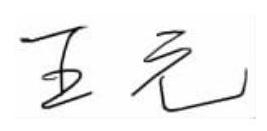
\includegraphics[max width=\textwidth, center]{2024_10_09_bce9f07034ef55fc9c97g-05}

\footnotetext{王元, 著名数学家, 中国科学院院士, 曾任中国数学会理事长、中国数学奥林匹克委员会主席.
}\begin{center}
\begin{tabular}{lll}
$\boldsymbol{1}$ & 计数问题 & 001 \\
$\mathbf{2}$ & 抽屉原理 & 013 \\
$\mathbf{3}$ & 染色问题 & 025 \\
$\mathbf{4}$ & 操作与游戏 & 036 \\
$\mathbf{5}$ & 组合最值 & 047 \\
\hline
 &  &  \\
\hline
 & 习题解答 & 066 \\
\hline
\end{tabular}
\end{center}

\footnotetext{001
}\section{计数问题}
计数方法种类繁多,本章旨在介绍一些基本方法.

\section{一、枚举计数}
枚举计数就是把要计数的对象一一列举出来, 最后计算总数的方法. 枚举计数的过程中, 必须注意不重复也不遗漏, 力求有序、有规律、逐一地进行。

例1 把 22 分成两个质数之和共有几种不同分法?\\
分析 设 $a+b=22$, 其中 $a 、 b$ 都是质数. 不妨设 $a \leqslant b$, 则 $a$ 可能取 2 、 3、5、7和 11 , 对每一个 $a$ 值, 若 $b$ 也是质数, 则得到一种分法.

解 设质数 $a 、 b$ 满足 $a \leqslant b, a+b=22$, 则 $a$ 可取 2、3、5、7和11. 当 $a=2$ 时, $b=20$, 不为质数; 当 $a=3$ 时, $b=19$, 为质数; 当 $a=5$ 时, $b=17$,为质数; 当 $a=7$ 时, $b=15$, 不为质数; 当 $a=11$ 时, $b=11$, 为质数. 故不同分法有 3 组, 即 $22=3+19=5+17=11+11$.

例 2 如图 1-1, 沿着边或对角线不重复地从 $A$走到 $D$, 一共有多少种走法 (这里不重复指走过的点和线段都不重复)?

解 不同走法有: $A \rightarrow D, A \rightarrow E \rightarrow D, A \rightarrow E \rightarrow C \rightarrow$ $D, A \rightarrow B \rightarrow C \rightarrow D, A \rightarrow B \rightarrow C \rightarrow E \rightarrow D$ 。一共有 5 种走法.

图 1 - 1\\
例 3 在一个网格纸(每个小方格都是边长为 1 的小正方形)中找出 4 个方格, 使得任一个选出的方格都可以通过所选方格的公共边到达另外三个方格, 则共有多少种不同选法( 通过平移和旋转可以重合的图形认为是相同的)?

解 依题意可以画出不同选法如下:

故一共有 7 种不同选法.\\
例4 在中国古代,有五行相克之说。五行即金、木、水、火、土,而相克是金克木、木克土、土克水、水克火、火克金,从五行中找出互不相克的两行,共有几种不同选法?

分析 我们可以用"金 $\rightarrow$ 木"来表示金克木,从而有金 $\rightarrow$ 木 $\rightarrow$ 土 $\rightarrow$ 水 $\rightarrow$火 $\rightarrow$ 金,于是可以枚举出所有的选法。

解 可以选择的两行可以是:(金,土),(金,水),(木,水),(木,火),(土,火). 一共五种。

在后面的例题中,我们可能会用到两个符号: $\mathrm{P}_{n}^{m}$ 及 $\mathrm{C}_{n}^{m}(m \leqslant n, m 、 n$ 均为自然数),下面介绍这两个符号表示的意思。\\
(1) $\mathrm{P}_{n}^{m}$ 表示从 $n$ 个元素中任取 $m$ 个元素的排列数。从 $n$ 个不同的元素中取 $m$ 个不同的元素按照一定次序排成一列,称为从 $n$ 个元素中取 $m$ 个元素的一个排列,所有这样不同排列的个数即为 $\mathrm{P}_{n}^{m}$ ,且\\
\begin{align*}
\mathrm{P}_{n}^{m}=n(n-1) \cdots(n-m+1)=\frac{n!}{(n-m)!}(m \leqslant n)
\end{align*}

其中 $n!=n(n-1) \cdot \cdots \cdot 2 \cdot 1$ ,并规定 $0!=1$ 。\\
证明如下: 设 $n$ 个元素为 $\left\{a_{i} \mid 1 \leqslant i \leqslant n\right\}$ ,而取的 $m$ 个元素的排列为 $b_{1}$ , $b_{2}, \cdots, b_{m}$ ,则 $b_{1}$ 可以是任一 $a_{j}(1 \leqslant j \leqslant n)$ ,故 $b_{1}$ 有 $n$ 种取法;而 $b_{1}$ 取定后, $b_{2}$只能取 $\left\{a_{i} \mid 1 \leqslant i \leqslant n\right\}$ 中除去 $b_{1}$ 后的任一元素,有 $n-1$ 种取法;类似地, $b_{3}$ 有 $n-2$ 种取法, $\cdots, b_{m}$ 有 $n-m+1$ 种取法,故 $b_{1}, b_{2}, \cdots, b_{m}$ 的取法有 $n(n-1) \cdots$ $(n-m+1)$ 种取法.\\
(2) $\mathrm{C}_{n}^{m}$ 表示从 $n$ 个元素中任取 $m$ 个元素的组合数。从 $n$ 个不同元素中取 $m$ 个元素,不论顺序如何并成一组,称为从 $n$ 个元素中取 $m$ 个元素的一个组合,所有这样不同组合的个数即为 $\mathrm{C}_{n}^{m}$ ,且\\
\begin{align*}
\mathrm{C}_{n}^{m}=\frac{\mathrm{P}_{n}^{m}}{m!}=\frac{n!}{m!(n-m)!}=\frac{n(n-1) \cdots(n-m+1)}{1 \times 2 \times \cdots \times m}
\end{align*}

证明如下:首先从 $n$ 个元素 $\left\{a_{i} \mid 1 \leqslant i \leqslant n\right\}$ 中选 $m$ 个元素的排列有 $\mathrm{P}_{n}^{m}$种,而对其中取定的 $m$ 个元素 $\left\{b_{i} \mid 1 \leqslant i \leqslant m\right\}$ 的排列数有 $\mathrm{P}_{m}^{m}=m$ !种,对于这 $m!$ 种不同的排列,它们的 $m$ 个元素都是相同,故属于同一个组合,所以从 $n$ 个元素中取 $m$ 个元素的组合个数有 $\frac{\mathrm{P}_{n}^{m}}{m!}$ 种。

例 5 求满足下列条件的所有五位数的个数:任意两个数位上的数字之差的绝对值不小于 2 。

分析 首先应该求出满足条件的五个数字,然后对每一组数字进行排列,即可求出所有满足条件的五位数的个数。

解 设五位数为 $\overline{a_{1} a_{2} a_{3} a_{4} a_{5}}$ ,设\\
\begin{align*}
\left\{b_{1}, b_{2}, b_{3}, b_{4}, b_{5}\right\}=\left\{a_{1}, a_{2}, a_{3}, a_{4}, a_{5}\right\}
\end{align*}

且 $b_{1}<b_{2}<b_{3}<b_{4}<b_{5}$. 由条件要求 $b_{1}$ 只能取 1 或 0 。\\
若 $b_{1}=1$ ,则必有 $b_{2}=3, b_{3}=5, b_{4}=7, b_{5}=9$ ,此时满足条件五位数 $\overline{a_{1} a_{2} a_{3} a_{4} a_{5}}$ 个数为 $\mathrm{P}_{5}^{5}=5!=120$ 。

若 $b_{1}=0$ 时,则 $\left\{b_{1}, b_{2}, b_{3}, b_{4}, b_{5}\right\}$ 可以为 $\{0,3,5,7,9\} 、\{0,2,5,7$ , $9\} 、\{0,2,4,7,9\} 、\{0,2,4,6,9\} 、\{0,2,4,6,8\}$ 共 5 组. 对于每一组 $\left\{b_{1}, b_{2}, b_{3}, b_{4}, b_{5}\right\}$, 由于 0 不能排在首位, $\overline{a_{1} a_{2} a_{3} a_{4} a_{5}}$ 的个数为\\
\begin{align*}
\mathrm{P}_{5}^{5}-\mathrm{P}_{4}^{4}=120-24=96
\end{align*}

从而共有 $96 \times 5=480$ 个。\\
所以满足条件的五位数的个数为 $(120+480=) 600$ 个。\\
例 6 在 1~2004中,有多少个整数可以表示为 $[2 x]+[4 x]+[6 x]$ 的形式,这里 $x$ 为实数。注: $[x]$ 是实数 $x$ 的高斯函数。

分析 设 $f(x)=[2 x]+[4 x]+[6 x]$ ,则一个很重要的结论是\\
\begin{align*}
\begin{aligned}
f\left(x+\frac{1}{2}\right) & =\left[2\left(x+\frac{1}{2}\right)\right]+\left[4\left(x+\frac{1}{2}\right)\right]+\left[6\left(x+\frac{1}{2}\right)\right] \\
& =[2 x+1]+[4 x+2]+[6 x+3] \\
& =f(x)+6
\end{aligned}
\end{align*}

即某一整数可用 $f(x)$ 表示,则这个数加上 6 也可由 $f(x)$ 的形式表示,于是我们只需求出 $1 \sim 6$ 中,有几个数可表示为 $f(x)$ 的形式。

解 设 $f(x)=[2 x]+[4 x]+[6 x]$ ,则 $f\left(x+\frac{1}{2}\right)=f(x)+6$ ,故若整数 $a$ 可表示为 $f(x)$ 形式,则 $a+6 k ( k \in \mathbf{N} )$ 也可表示为 $f(x)$ 形式,所以只需求得 $1 \sim 6$ 中有几个数可表示成 $f(x)$ 形式。

当 $x \in\left[0, \frac{1}{6}\right)$ 时, $f(x)=0$ ;\\
当 $x \in\left[\frac{1}{6}, \frac{1}{4}\right)$ 时, $f(x)=1$ ;\\
当 $x \in\left[\frac{1}{4}, \frac{1}{3}\right)$ 时, $f(x)=2$ ;\\
当 $x \in\left[\frac{1}{3}, \frac{1}{2}\right)$ 时, $f(x)=3$ ;

又 $f\left(\frac{1}{2}\right)=6$, 因此 $1 \sim 6$ 中, 有 $1 、 2 、 3 、 6$ 可表示为 $f(x)$ 的形式,故 $1 \sim$ 2004 中有 $2004 \div 6 \times 4=1336$ 个数可表示为 $f(x)$ 的形式。

例7 设正整数 $a_{1} 、 a_{2} 、 a_{3} 、 a_{4} 、 a_{5}$ 满足条件:\\
(1) $1 \leqslant a_{1}<a_{2}<a_{3}<a_{4}<a_{5} \leqslant 20$;\\
(2) 任意两个数之差不小于 3 .

求这样的数组 $\left\{a_{1}, a_{2}, a_{3}, a_{4}, a_{5}\right\}$ 的组数.\\
分析 依题意有 $a_{5}>a_{4}+2, a_{4}>a_{3}+2, a_{3}>a_{2}+2, a_{2}>a_{1}+2$, 即 $a_{5}>a_{4}+2>a_{3}+4>a_{2}+6>a_{1}+8 \geqslant 9$, 故 $\left\{a_{5}, a_{4}+2, a_{3}+4, a_{2}+6\right.$, $\left.a_{4}+8\right\}$ 为 $9 \sim 20$ 内不同的 5 个数, 而相应的, 由 $9 \sim 20$ 内 5 个不同数也可以对应于 $a_{5}, a_{4}+2, a_{3}+4, a_{2}+6, a_{1}+8$ 。

解 依题意有 $9 \leqslant a_{1}+8<a_{2}+6<a_{3}+4<a_{4}+2<a_{5} \leqslant 20$, 而对于 9 20 中五个数 $b_{1}<b_{2}<b_{3}<b_{4}<b_{5}$, 则 $b_{1}-8, b_{2}-6, b_{3}-4, b_{4}-2$, $b_{5}$ 满足条件 (1)、(2), 即满足条件 (1)、(2) 的 $\left\{a_{1}, a_{2}, a_{3}, a_{4}, a_{5}\right\}$ 的个数为从 $9 \sim 20$ 中取 5 数组的组数, 也即 $\mathrm{C}_{12}^{5}=792$.

例 8 设开始 $A=0$. 将一枚硬币郑出, 若郑得正面, 则 $A$ 加上 1 , 否则 $A$减去 1 . 当 $A=3$ 或郑出次数达到 7 次时就不再掷了. 问当掷币停止时, 不同郑币情况有多少种?

分析 当郑币停止了, 要么 $A=3$, 掷出次数不超; 要么 $A \leqslant 2$, 且郑出次数已达到 7 次. 若 $A=3$, 则最后一次必为正面, 前面可以是 2 次正面或 3 次正面 1 次反面或 4 次正面 2 次反面; 若 $A$ 一直不大于 2 , 则当第 7 次郑出时, 停止掷币.

解 若 $A=3$ 且仅掷了 3 次, 此时 3 次全为正面, 即仅有 1 种方法;\\
若 $A=3$ 且掷了 5 次, 则前 4 次为 3 次正面、 1 次反面. 但如果前 3 次已全部是正面, 则 $A$ 已达到了3, 故一次反面必出现在前 3 次中, 所以有 3 种郑法;

若郑了 7 次才停止, 则前 6 次掷后 $A$ 不大于 2 , 此时有:\\
(i) 4 次正面、 2 次反面. 此时不能前 3 次均为正面,也不能前 5 次为 4 次正面一次反面,故可能的郑法有 $\left(\mathrm{C}_{6}^{2}-3-3=\right) 9$ 种;\\
(ii) 3 次正面、 3 次反面. 此时不能前 3 次均为正面, 故可能的郑法有 ( $\left.\mathrm{C}_{6}^{3}-1=\right) 19$ 种;\\
(iii) 2 次正面、4 次反面或 1 次正面、 5 次反面或全为反面, 共有郑法 $\left(\mathrm{C}_{6}^{2}+\mathrm{C}_{6}^{1}+\mathrm{C}_{6}^{0}=\right) 22$ 种。

但第 7 次郑出有正、反面两种,故共有 $((9+19+22) \times 2=) 100$ 种郑法.\\
综上, 共有不同郑法 $(1+3+100=) 104$ 种.\\
例 9 有 3 个红球和 8 个蓝球排成一圈,任意两个红球之间至少有两个

蓝球,问共有多少种不同排列方法(只要把圆旋转一下就重合的排法认为是同一种)?

分析 我们可以将红球和在它逆时针方向相邻的两个蓝球看成一个整体,例如当成一个白球,这样问题就转化为 3 个白球和两个蓝球的不同圆排列方法.

解 由于任意两个红球之间至少有两个蓝球,故每个红球的逆时针方向相邻的位置至少有两个蓝球,于是,将每个红球和它逆时针方向相邻的两个蓝球看成一个球,如白球,则满足条件的排列与三个白球、两个蓝球的圆排列是一一映射的。

而三个白球、两个蓝球的圆排列的不同排列方法有 2 种(枚举即可),故所求的不同排列种类为 2 种。

例 10 袋中装有红、白球各 3 个,从袋中拿出球,每次拿一个,要求拿出的白球个数不得多于红球,问有多少种不同拿法?

分析 由于要求拿出的白球个数不多于红球,故第一个球必是红球。而若最后一球为红球,则拿出第 5 个球时白球数大于红球数,故第 6 个球必为白球。其他 4 个球可以利用枚举法枚举.

解 依题意知,第 1 个球必为红球,第 6 个球必为白球,而其余 4 个球的不同拿法有:红红白白、红白红白、红白白红、白红红白、白红白红,一共有 5 种不同拿法.

例 11 求 100 以内仅能分解为两个素数之积的正整数的个数.\\
分析 可以对 $1 \sim 100$ 进行因数分解,然后找出符合条件的数;也可以用两个素数相乘,将 100 以内的数挑出来. 显然,后一种方法简单一些.

解 50 以内素数有 $2 、 3 、 5 、 7 、 11 、 13 、 17 、 19 、 23 、 29 、 31 、 37 、 41 、$ 43、 47 共 15 个. 设分解素因数后为 $a \times b$ ,其中 $a \leqslant b$ 。

若 $a=2$ ,则 $b$ 可取这 15 个素数,即有 15 个数;\\
若 $a=3$ ,则 $b$ 可取 $3 \sim 31$ 这 10 个素数,即有 10 个数;\\
若 $a=5$ ,则 $b$ 可取 $5 \sim 19$ 这 6 个素数,即有 6 个数;\\
若 $a=7$ ,则 $b$ 可取 $7 、 11 、 13$ 共 3 个素数,即有 3 个数;\\
若 $a \geqslant 11$ ,则 $a \times b \geqslant 11 \times 11=121>100$ ,不满足要求。\\
综上,满足条件的数有 $(15+10+6+3=) 34$ 个。

\section{二、分类思想与加法原理}
加法原理是指完成—件事情可以分为 $m$ 类,第 1 类有 $n_{1}$ 种方法,第 2 类有 $n_{2}$ 种方法 $\cdots \cdots$ 第 $m$ 类有 $n_{m}$ 种方法,则完成这件事情的不同方法的总数为\\
\begin{align*}
N=n_{1}+n_{2}+\cdots+n_{m}
\end{align*}

例 12 一位解放军打靶,他打了 3 枪,共 21 环,而每枪可以打 $1 \sim 10$ 环,问他有多少种不同的打法(要求考虑打枪的次序)?

分析 设三枪分别为 $a 、 b 、 c$ 环,则 $1 \leqslant a, b, c \leqslant 10, a+b+c=21$ ,于是 $\max (a, b, c) \geqslant 7$ 。将 $\{a, b, c\}$ 重排列为 $\left\{a^{\prime}, b^{\prime}, c^{\prime}\right\}$ 且 $a^{\prime} \leqslant b^{\prime} \leqslant c^{\prime}$ 。对 $c^{\prime}=7,8,9,10$ 分类讨论即可得到总的打法数.

解 设三枪依次为 $a 、 b 、 c$ 环,对 $\{a, b, c\}$ 重新排列为 $\left\{a^{\prime}, b^{\prime}, c^{\prime}\right\}$ 且 $a^{\prime} \leqslant$ $b^{\prime} \leqslant c^{\prime}$.

若 $c^{\prime}=7$ ,则 $a^{\prime}=b^{\prime}=7$ ,此时共有 1 种打法。\\
若 $c^{\prime}=8$ ,则 $\left(a^{\prime}, b^{\prime}\right)$ 可取 $(5,8) 、(6,7)$ 。当 $\left(a^{\prime}, b^{\prime}\right)=(5,8)$ 时,有 3 种打法;当 $\left(a^{\prime}, b^{\prime}\right)=(6,7)$ 时,有 $\left(\mathrm{P}_{3}^{3}=\right) 6$ 种打法。即共有 9 种打法。

若 $c^{\prime}=9$ ,则 $\left(a^{\prime}, b^{\prime}\right)$ 可取 $(3,9) 、(4,8) 、(5,7) 、(6,6)$ 。当 $\left(a^{\prime}, b^{\prime}\right)=$ $(3,9)$ 或 $(6,6)$ 时,各有 3 种打法;当 $\left(a^{\prime}, b^{\prime}\right)=(4,8)$ 或 $(5,7)$ 时,各有 6 种打法. 即共有 18 种打法.

若 $c^{\prime}=10$ ,则 $\left(a^{\prime}, b^{\prime}\right)$ 可取( 1,10$) 、(2,9) 、(3,8) 、(4,7) 、(5,6)$ 。当 $\left(a^{\prime}, b^{\prime}\right)=(1,10)$ 时,有 3 种打法;当 $\left(a^{\prime}, b^{\prime}\right)$ 取其他值时,各有 6 种打法。即共有 $(3+6 \times 4=) 27$ 种打法。

综上,由加法原理,一共有 $(1+9+18+27=) 55$ 种不同打法。\\
例13 由 1、2、3这3个数组成六位数,要求相邻数位上的数字都不相同,有多少个满足条件的六位数?

分析 依题意知,不可能有一个数字出现在 4 个数位上,所以可能是两个数字分别出现 3 次,也可能是三个数字分别出现 $1 、 2 、 3$ 次或者 $2 、 2 、 2$ 次,再用加法原理对上述三种可能下的个数求和即可。

解 依题意知,不可能有某个数字出现在 4 个数位上,故每个数字至多出现 3 次。

若为两个数字各出现 3 次,那么两个数字必间隔排列,即有 2 个不同的六位数。而这两个数字可以是 $(1,2) 、(1,3)$ 或 $(2,3)$ ,故有 $(2 \times 3=) 6$ 个不同的六位数。

若为三个数字且分别出现 $1 、 2 、 3$ 次,首先各个数字出现次数不同的情况共有 $\left(\mathrm{P}_{3}^{3}=\right) 6$ 种。对于其中任一种,不妨设 1 出现 3 次,2出现 2 次,3出现 1次,先将两个 2 与一个 3 排成一排(有 3 种排法)再与 3 个 1 间隔排列,可得 ( $3 \times 2=) 6$ 个六位数;又将一个 2 和一个 3 组合,再和另一个 2 放在 3 个 1 的三个数位之间,可得 $121231 、 121321 、 123121 、 132121$ 等 4 个六位数. 故共有 $(6 \times(6+4)=) 60$ 个不同的六位数。

若为三个数字各出现 2 次,首先前两位是从 3 个数字中选 2 个排列,共有 $\left(P_{3}^{2}=\right) 6$ 种排法;再设前两位为 12 ,则后四位可以为 $1323 、 3123 、 3132 、 3213$ 、 3231 共 5 种,故不同的六位数共有 $(6 \times 5=) 30$ 个。

综上,由加法原理可知,一共有满足条件的六位数 $(6+60+30=) 96$ 个。\\
简解: $3 \times 2^{5}=96$ 。\\
例14 在一个五条边长各不相同的五边形的边上染色,每条边可以染红、黄、蓝三种颜色中的一种,但不允许相邻边有相同颜色,问有多少种不同染色法?

分析 不妨将边编号为 $a 、 b 、 c 、 d 、 e, a b 、 b c 、 c d 、 d e 、 e a$ 为相邻边,则先不妨设 $a 、 b$ 分别为红、黄色,再对后面三条边染色,则可得到所有不同染色方法.

解 将五条边依次编号为 $a 、 b 、 c 、 d 、 e$. 先假定 $a$ 为红色, $b$ 为黄色,则:\\
若 $c$ 为红色,则 $(d, e)$ 可以为(黄、蓝)、(蓝、黄);\\
若 $c$ 为蓝色, 则 $(d, e)$ 可以为(红, 黄)、(红, 蓝)、(黄, 蓝)。\\
由加法原理知,当 $(a, b)$ 为(红,黄)时,共有 $(2+3=) 5$ 种染色法。\\
而 $(a, b)$ 还可以为(红,蓝)、(黄,蓝)、(黄,红)、(蓝,红)、(蓝,黄),而每一种情况下都是对称的,故不同染色法总共有 $(5 \times 6=) 30$ 种.

例 15 某届运动会的十一天的比赛中, $\times$ 队队拿了 16 块金牌,其中每天至少有一枚金牌,则 $\times \times$ 队拿金牌的不同情况可能有多少种(假设金牌都是一样的)?

分析 由于每天至少有一块金牌,则先给每天分配一块金牌,剩下的五块金牌如何分配就决定了不同的情况。

解 设第 $i(1 \leqslant i \leqslant 11)$ 天取得 $a_{i}+1$ 块金牌,则\\
\begin{align*}
a_{i} \geqslant 0, \sum_{i=1}^{11} a_{i}=5
\end{align*}

若 $\left\{a_{i}\right\}$ 中有一个为 5 ,则有 $\left(\mathrm{P}_{11}^{1}=\right) 11$ 种方法;\\
若 $\left\{a_{i}\right\}$ 中有 4 和 1 ,或 3 和 2 ,则各有 $\left(\mathrm{P}_{11}^{2}=\right) 110$ 种,于是共有 $(110 \times 2=)$ 220 种;

若 $\left\{a_{i}\right\}$ 中有 3、1、1,或 2、2、1,则各有 $\left(\frac{\mathrm{P}_{11}^{3}}{2!}=\right) 495$ 种,于是共有 $(495 \times$ $2=) 990$ 种方法;

若 $\left\{a_{i}\right\}$ 中有 2、1、1、1, 则有 $\left(\frac{\mathrm{P}_{11}^{4}}{3!}=\right) 1320$ 种;\\
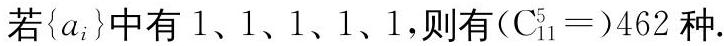
\includegraphics[max width=\textwidth, center]{2024_10_09_bce9f07034ef55fc9c97g-13}

综上,由加法原理知, $\times$ ×队拿金牌的不同可能情况有 $11+220+990+$ $1320+462=3003$ 种.

简解:挡板原理: $n$ 个正整数和为 $m(m \geqslant n)$ ,不同选法种类数为 $C_{m-1}^{n-1}$ 。本题中 $m=16, n=11$ ,所以 $\mathrm{C}_{16-1}^{11-1}=\mathrm{C}_{15}^{10}$ 。

例16 工厂需要3名钳工和 3 名车工,现有 12 人可供挑选,其中 5 人会钳工, 5 人会车工,还有 2 人既会钳工也会车工,问工厂有多少种不同的挑选方法?

分析 解决问题的关键是确定两个既会钳工又会车工的工人是做钳工还是做车工,或是不被挑选,然后运用加法原理即可求出所有不同的挑选方法。

解 设既会钳工又会车工的两人为 $a 、 b$.\\
若 $a 、 b$ 均未被挑选,则不同方法有 $\left(\mathrm{C}_{5}^{3} \cdot \mathrm{C}_{5}^{3}=\right) 100$ 种;\\
若 $a 、 b$ 有一人做钳工,则不同方法有 $\left(\mathrm{C}_{2}^{1} \cdot \mathrm{C}_{5}^{2} \cdot \mathrm{C}_{5}^{3}=\right) 200$ 种;\\
若 $a 、 b$ 有一人做车工,也有不同方法 200 种;\\
若 $a 、 b$ 两人均做钳工,则不同方法有 $\left(\mathrm{C}_{5}^{1} \cdot \mathrm{C}_{5}^{3}=\right) 50$ 种;\\
若 $a 、 b$ 两人均做车工,则不同方法也有 50 种;\\
若 $a 、 b$ 一人做钳工,一人做车工,则不同方法有 $\left(\mathrm{P}_{2}^{2} \cdot \mathrm{C}_{5}^{2} \cdot \mathrm{C}_{5}^{2}=\right) 200$ 种。\\
综上,由加法原理知,工厂不同的挑选方法有 $(100+200+200+50+$ $50+200=) 800$ 种。

例17 形如" $313 " , " 72427 "$ 的正整数称为回文数,即这个数的各个数位前后颠倒过来后仍是这个数,求 1 亿内的回文数的个数。

分析 设回文数有 $k$ 位,则前 $\left[\frac{k+1}{2}\right]$ 位确定后,则后 $\left[\frac{k}{2}\right]$ 位也随之确定,即 $k$ 位回文数对应于 $\left[\frac{k+1}{2}\right]$ 位的所有数,再利用加法原理,对 $k(=1,2, \cdots$ , 8)位回文数的个数求和即得所求回文数的个数.

解 设回文数有 $k$ 位 $(1 \leqslant k \leqslant 8)$ ,则该 $k$ 位回文数与它的前 $\left[\frac{k+1}{2}\right]$ 位组成的数一一对应.

若 $k=1$ ,则有 9 个回文数;\\
若 $k=2$ ,则 $\left[\frac{k+1}{2}\right]=1$ ,即可取 9 个回文数;\\
若 $k=3$ ,则 $\left[\frac{k+1}{2}\right]=2$ ,即可取 90 个回文数;\\
若 $k=4$ ,则 $\left[\frac{k+1}{2}\right]=2$ ,即可取 90 个回文数;

若 $k=5$ ,则 $\left[\frac{k+1}{2}\right]=3$ ,即可取 900 个回文数;\\
若 $k=6$ ,则 $\left[\frac{k+1}{2}\right]=3$ ,即可取 900 个回文数;\\
若 $k=7$ ,则 $\left[\frac{k+1}{2}\right]=4$ ,即可取 9000 个回文数;\\
若 $k=8$ ,则 $\left[\frac{k+1}{2}\right]=4$ ,即可取 9000 个回文数.\\
综上,由加法原理知, 1 亿内共有回文数 $(9+9+90+90+900+900+$ $9000+9000=) 19998$ 个。

例18 某足球队参加足球比赛,现在该队有 11 名队员在场上踢比赛,在场下还有 7 名替补队员。比赛规定,比赛中,可以从替补队员中挑队员与场上队员交换替补上场,但至多可以换 3 名队员,而且已经换下的队员不能再替补上场。如果整场比赛中没有队员被罚下,则比赛结束时,场上的 11 名队员的不同情况有多少种?

分析 依题意知,有可能留在场上的替补队员个数为 $0 、 1 、 2 、 3$ 。\\
解 若没有替补队员被替换上场,则有 1 种情况;\\
若有 1 名队员被替换上场,则有 $\left(\mathrm{C}_{7}^{1} \times \mathrm{C}_{11}^{1}=\right) 77$ 种情况;\\
若有 2 名队员被替换上场,则有 $\left(\mathrm{C}_{11}^{2} \times \mathrm{C}_{7}^{2}=\right) 1155$ 种;\\
若有 3 名队员被替换上场,则有 $\left(\mathrm{C}_{11}^{3} \times \mathrm{C}_{7}^{3}=\right) 5775$ 种。\\
综上,由加法原理知共有不同情况 $(1+77+1155+5775=) 7008$ 种。

\section{三、分步处理与乘法原理}
乘法原理是指完成一件事情要分 $m$ 步,第 1 步有 $n_{1}$ 种方法,第 2 步有 $n_{2}$种方法 $\cdots \cdots$ 第 $m$ 步有 $n_{m}$ 种方法,则完成这件事情的不同方法的总数为\\
\begin{align*}
N=n_{1} \times n_{2} \times \cdots \times n_{m}
\end{align*}

例19 所有含有数字 2 和 6 的六位数中, 2 和 6 都仅含有一个的数有多少个?

分析 由于 2 和 6 出现且仅出现一次,其他 4 位可以是数字 $0 、 1 、 3 、 4$ 、 $5 、 7 、 8 、 9$ ,而第一个数位不能为 0 ,利用乘法原理和加法原理即可求出所有满足条件的六位数的个数。

解 若 2 和 6 不出现在首位,则首位可取 7 个数,其他不为 2 和 6 的三位各可取 8 个数,故有 $\left(\mathrm{P}_{5}^{2} \times 8^{3} \times 7=\right) 71680$ 个;

若 2 和 6 出现在首位, 则首位可以是 2 或 6 ,故有 $\left(2 \times \mathrm{C}_{5}^{1} \times 8^{4}=\right)$ 40960 个。

综上,所求六位数共有 $(71680+40960=) 112640$ 个.\\
例20 在 $10 \times 10$ 的棋盘上放红、黄、蓝各一子,若黄子与红子不能同列,蓝子与黄子不能同行,则共有多少种不同的摆法(任两子均不能重叠放置)?

分析 依次将三个棋子分别放到棋盘上,分别计算放的方法,利用乘法原理即得所求结果. 其中,先放红子和蓝子,再放黄子,计算较为方便。

解 先放红子,有 100 种放置方法;再放蓝子,由于不能重叠放置,所以有红子位置以外的 99 种放置方法;最后放黄子,由于黄子与红子不同列,与蓝子不同行,故可在其余 9 行、 9 列中放置,有 81 种放置方法。根据分步处理的乘法原理,总的摆法有 $(100 \times 99 \times 81=) 801900$ 种。

例 21 求满足下列两条件的所有八位数个数:\\
(1)每个数位的数字为 $1 \sim 9$ 中某一个;\\
(2)任意连续三个数位组成的三位数能被 3 整除。\\
分析 一个数能被 3 整除的充要条件是该数各个数位上的数字之和能被 3 整除,从这个事实出发并利用乘法原理我们即可求出所有满足条件的八位数个数。

解 首先说明一个事实,即三位数仅由数字 $1 \sim 9$ 组成,且能被 3 整除,若前两数位已确定,则这个三位数的第 3 位有且仅有 3 个可能值。事实上,设前两个数位之和为 $a$ ,则当 $a \equiv 0(\bmod 3)$ 时,第 3 位可取 3、 $6 、 9$ ;当 $a \equiv 1(\bmod 3)$时,第 3 位可取 $2 、 5 、 8$ ;当 $a \equiv 2 ( \bmod 3 )$ 时,第 3 位可取 $1 、 4 、 7$ 。

于是,满足条件的八位数的首位可以取 9 个值,而第 2 位可取 9 个值,当前两位已确定后,由前面提到的事实知,后面 6 位上每个数位上的可能值均为 3 个,从而由乘法原理知,满足条件的八位数有 $\left(9 \times 9 \times 3^{6}=\right) 59049$ 个。\\
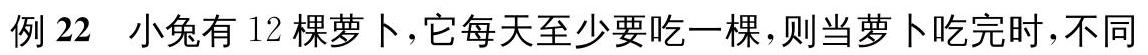
\includegraphics[max width=\textwidth]{2024_10_09_bce9f07034ef55fc9c97g-16}的吃萝卜的情形有多少种?

分析 由于不能确定几天吃完,而且前几天吃夢卜的个数对后几天又有影响,所以用枚举是不太现实的。我们可以用递归加上数学归纳法求,也可以将问题转化为另一个问题,用一一映射来求。

解法 1 若将题设中 12 改为 $n$ ,所求吃萝卜的情形有 $F(n)$ 种,则 $F(1)=1, F(2)=2, F(3)=4$ 。我们猜想: $F(n)=2^{n-1}\left(n \in \mathbf{N}^{*}\right)$ 。

当 $n \leqslant 3$ 时, $F(n)=2^{n-1}$ 成立;\\
若当 $n \leqslant k$ 时均成立,则当 $n=k+1$ 时,若第一天吃 $i(1 \leqslant i \leqslant k+1)$ ,则此时不同吃法为 $F(k+1-i)$ (记 $F(0)=1$ ),于是所有不同吃法为\\
\begin{align*}
F(n)=\sum_{i=1}^{k+1} F(k+1-i)=\sum_{i=0}^{k} F(i)=1+\sum_{i=1}^{k} 2^{i-1}=2^{k+1}
\end{align*}

即对 $n=k+1$ 也成立,由数学归纳法知, $F(n)=2^{n-1}\left(n \in \mathbf{N}^{*}\right)$ 。\\
对于本题, $n=12$, 则所求为 $F(12)=2^{11}=2048$ 。\\
解法 2 将 12 棵萝卜一字排开,编号为 $1 \sim 12$ 号,小兔吃萝卜从 1 号开始依次吃,若某天最后吃完的是第 $k$ 棵萝卜,则在第 $k$ 棵萝卜后放一根筷子 (其中 $1 \leqslant k \leqslant 11$ )。因此对于每一种吃法,对应有若干根筷子在若干棵萝卜后,而对于筷子的每一种放法,对应一种吃萝卜的方法,即这种对应为一一映射. 于是问题转化为在 11 个位置上放筷子(每个位置至多放一根筷子),有多少种放法而每个位置,可以放筷子,也可以不放筷子,根据乘法原理知,不同的放筷子的方法有 $\left(2^{11}=\right) 2048$ 种,即不同的吃萝卜的方法有 2048 种。

例23 甲地到乙地有 5 条不同的路,某人从甲地到乙地,然后从乙地返回,再又去乙地,再又返回甲地,要求返回时不能走任何一次去乙地的路,问此人有多少种不同走法?

分析 运用乘法原理可解此题,但要考虑第二次从甲地到乙地的路是否与第一次从甲地到乙地的路重叠。

解 第一次从甲地到乙地有 5 种选择,从乙地回到甲地有 4 种选择,此时若第二次到乙地的路与第一次重叠,则返回时有 4 种选择;

若第二次到乙地不与第一次重叠,则有 4 种不同选择,而此时返回时有 3种选择.

于是,由乘法原理和加法原理有 $5 \times 4 \times(4+4 \times 3)=320$ 种不同走法。

例 24 在 $1 \times n$ 的方格内写数字 $1 \sim n$ ,要求 2 和 1 相邻,当 $1 \sim k ( 2 \leqslant k \leqslant$ $n-1)$ 填好后, $k+1$ 必须与已写好的数相邻,问有多少种不同填数方法。

解 依题意知 $n$ 必定在最前或最后的方格中,故 $n$ 可能有两种填法,而当 $n$ 写好后, $n-1$ 也有两种填法 $\cdots \cdots$ 直到 2 也有两种填法,最后一个格子填上 1. 而这样的填法也包含有所有的不同填法, 故由乘法原理知,必有 $2^{n-1}$ 种不同填法.

例2512个元素的集合中选出4个3元子集,任两个 3 元子集均无交集,则不同取法有多少种?

解 第一步取出一个 3 元子集有 $\mathrm{C}_{12}^{3}$ 种取法,第二步从剩下 9 个数中取 3个,有 $\mathrm{C}_{9}^{3}$ 种取法,第三步取出一个 3 元子集有 $\mathrm{C}_{6}^{3}$ 种方法,最后剩下一个 3 元子集。由于不考虑顺序,故由乘法原理知共有 $\left(\frac{1}{4!} \cdot C_{12}^{3} \cdot C_{9}^{3} \cdot C_{6}^{3}=\right) 15400$ 种不同取法.

\section{习题 1}
13 个红球和 3 个蓝球围成一圈,不同的排列方式有几种(旋转后可重合的算同一种)?\\
2 将数 1 5 排成一排, 使任意 3 个相邻的数都不单调的不同排列个数有多少个?

31 个红球、 2 个黄球和 3 个蓝球排成一列,没有两个同色球排在相邻位置上的不同排列有多少个?\\
4 将 $1 \sim 5$ 排成一排,每个数均不大于它两侧(如果两侧都有数的话)的两个数的平均数,问这样的排列有多少个?\\
5 四个数 1、2、3、4的排列 $\left\{a_{1}, a_{2}, a_{3}, a_{4}\right\}$ 中,使任一个 $i(1 \leqslant i \leqslant 4)$ 都有 $a_{i} \neq i$ 的不同排列的个数有多少个?\\
6 在 $1 \sim 12$ 中找出 3 个数,使得这 3 个数是某个公差大于 2 的等差数列中 3项,则不同的取法有多少项?\\
7 在 $10 \times 10$ 的方格纸中选出若干个方格,组成一个正方形方格块,则不同的取法有多少种?\\
8 用 4 种给定颜色中的若干种染一个正方体,如果每个面涂一个颜色,而且相邻的面涂不同颜色,问有多少种不同涂法(若正方体经若干次翻转后相同视为同一种染法)?

9 长与宽是互质的正整数,面积是 20 !的矩形有多少个?\\
10 设 $a 、 b 、 c$ 是 $0 \sim 9$ 的数字,将循环小数 $0 . \dot{a} b \dot{c}$ 化成最简分数后,分子有多少种不同情况?

抽屉原理的最简单形式如下:\\
若把 $n+1$ 个苹果放入 $n$ 个不同的盒子中, 则至少有一个盒子里有两个或两个以上的苹果.

上述抽屉原理首先由 $\operatorname{Dirichlet}(1805-1859)$ 提出并在数论问题中使用.随后, 更进一步地归纳为下述三种形式:

抽屉原理I 把 $n+1$ 个元素按照任意确定的方式划分成 $n$ 个集合, 那么一定存在某个集合含有两个或两个以上的元素.

抽屉原理II 把 $m$ 个元素按照任意确定的方式划分成 $n$ 个集合 $(m 、 n$ 为正整数), 那么一定存在某个集合含有 $\left[\frac{m-1}{n}\right]+1$ 个或 $\left[\frac{m-1}{n}\right]+1$ 个以上的元素.

抽屉原理III 把无穷多个元素按照任意确定的方式划分成有限个集合,那么一定存在某个集合含有无穷多个元素.

抽屉原理II的证明 用反证法。假设每个集合中至多含有 $\left[\frac{m-1}{n}\right]$ 个元素, 则 $n$ 个集合中至多含有 $n \cdot\left[\frac{m-1}{n}\right]$ 个元素.又\\
\begin{align*}
n \cdot\left[\frac{m-1}{n}\right] \leqslant n \cdot \frac{m-1}{n}=m-1
\end{align*}

即 $n$ 个集合中至多含有 $m-1$ 个元素, 这与已知条件有 $m$ 个元素放入 $n$ 个集合中,矛盾!假设不成立,故结论成立。

抽屉原理 I 和III的证明仿上可用反证法给出证明.\\
用抽屉原理解答数学问题的策略是:分析题意,构造"苹果"和"抽屉",应用抽屉原理中某种形式. 而应用抽屉原理解决问题的关键是恰到好处地构造 "苹果"或"抽屉". 构造"抽屉"的方式有很多, 如:剩余类、区间、几何图形、染色类等.

例1 任给 12 个整数, 证明: 其中必存在 8 个数, 将它们用适当的运算符

号连起来后运算的结果是 3465 的倍数.\\
分析 注意到 $3465=11 \times 9 \times 7 \times 5$ ,由此可以联想到利用余数构造抽屉。

证明 一个整数被 11 除后的余数分别是 $0,1,2, \cdots, 10$,即剩余类构成 11 个抽屉. 由抽屉原理, 12 个整数中必有两个数在同一剩余类, 记为 $a_{1} 、 a_{2}$,则 $11 \mid\left(a_{1}-a_{2}\right)$.

12 个整数中去掉 $a_{1} 、 a_{2}$ 后,剩下 10 个整数. 这 10 个整数分入 9 的剩余类 (共九个抽屉) 中, 由抽屉原理,必有两个数在同一剩余类, 记为 $a_{3} 、 a_{4}$, 则 $9 \mid\left(a_{3}-a_{4}\right)$ 。

剩下的 8 个整数分入 7 的剩余类, 由抽屉原理,必有两个数在同一剩余类, 记为 $a_{5} 、 a_{6}$, 则 $7 \mid\left(a_{5}-a_{6}\right)$ 。

最后余下的 6 个整数分入 5 的剩余类, 由抽屉原理,必有两个数在同一剩余类, 记为 $a_{7} 、 a_{8}$, 则 $5 \mid\left(a_{7}-a_{8}\right)$.

因此, $\left(a_{1}-a_{2}\right)\left(a_{3}-a_{4}\right)\left(a_{5}-a_{6}\right)\left(a_{7}-a_{8}\right)$ 能被 3465 整除, 即存在 8 个数, 将它们用适当的运算符号连起来后, 运算的结果是 3465 的倍数.

注 这里构造的"抽屉"是"剩余类"。\\
例 2 从 1 至 138 共 138 个正整数中任取 11 个互异的数, 证明: 在取定的 11 个数中一定有两个互异的正整数, 它们的比值 $k$ 满足 $\frac{2}{3} \leqslant k \leqslant \frac{3}{2}$.

分析 将 1 138 的正整数分组 (即构造抽屉), 满足同一组中任意两数的比值介于 $\frac{2}{3}$ 至 $\frac{3}{2}$ 之间,且组数不多于 10 个。

证明 将 1 至 138 共 138 个正整数分成 10 组,即\\
\begin{align*}
\begin{aligned}
& A_{1}\{1\}, A_{2}=\{2,3\}, A_{3}=\{4,5,6\}, A_{4}=\{7,8,9,10\} \\
& A_{5}=\{11,12, \cdots, 16\}, A_{6}=\{17,18, \cdots, 25\} \\
& A_{7}=\{26,27, \cdots, 39\}, A_{8}=\{40,41, \cdots, 60\} \\
& A_{9}=\{61,62, \cdots, 91\}, A_{10}=\{92,93, \cdots, 138\}
\end{aligned}
\end{align*}

其中同一组中任意两数比值介于 $\frac{2}{3}$ 至 $\frac{3}{2}$ 之间(事实上,只须证明每组中最大数与最小数之比不超过 $\frac{3}{2}$, 即 $\frac{6}{4}=\frac{3}{2}, \frac{10}{7}<\frac{3}{2}, \frac{16}{11}<\frac{3}{2}, \frac{25}{17}<\frac{3}{2}, \frac{39}{26}=\frac{3}{2}$, $\frac{60}{40}=\frac{3}{2}, \frac{91}{61}<\frac{3}{2}, \frac{138}{92}=\frac{3}{2}$ ).

由抽屉原理知, 任取 11 个数中至少有两个数属于同一组, 从而这两个数之比介于 $\frac{2}{3}$ 至 $\frac{3}{2}$ 之间。

注 这里构造的"抽屉"是"区间"。\\
例 3 在 $3 \times 4$ 的长方形中, 任意放置 6 个点. 证明: 可以找到两个点, 它们的距离不大于 $\sqrt{5}$.

分析 若简单地设计抽屉为 $1 \times 2$ 的长方形, 这时每个区域内两点距离不超过其对角线之长 $\sqrt{5}$. 但此时共有 6 个抽屉, 还不能用抽屉原理. 因此, 必须改变抽屉形状, 一共只构造五个抽屉, 且使每个抽屉内任意两点间的距离不大于 $\sqrt{5}$ 。

证明 如图 2-1, 把长方形划分为 5 个区域:五边形 $A A_{1} A_{2} D_{2} D_{1}$ 、五边形 $A_{1} B B_{1} B_{2} A_{2}$ 、五边形 $A_{2} B_{2} C_{1} C_{2} D_{2}$ 、四边形 $D_{1} D_{2} C_{2} D$ 、四边形 $B_{1} C C_{1} B_{2}$.这五个区域形状有两类,而每个区域中任意两点之间的距离都不超过它们的最长对角线之长 $\sqrt{5}$ 。因此 6 个点放入此长方形内, 必有两点在同一区域, 从而

图 2 - 1它们的距离不大于 $\sqrt{5}$.

注 这里构造的"抽屉"是"几何图形".\\
例 4 在 5 列 33 行的方格棋盘上染色, 每格或染黑色或染白色, 证明: 至少有两行染的颜色完全一样.

分析 由于所证为至少有两行染的颜色一样, 故抽屉应为一行方格的不同染法. 由于一行有 5 格,故有 $\left(2^{5}=\right) 32$ 种不同染法.

证明 对某一行,此行由 5 格组成,每格可染黑色或白色,故有 $\left(2^{5}=\right) 32$种不同染法.

但现有 33 行, 故由抽屉原理知, 必存在两行, 它们染的颜色是一样的.\\
注 这里构造的"抽屈"是"染色类".

构造"抽屉"的形式是多样的,再通过下面的例子提高我们构造"抽屉"解决问题的能力.

例 5 某班有 60 人, 任意两人要么相互认识, 要么相互不认识, 证明: 必有两个人, 他们认识的人的个数是一样的.

分析 由于证明存在两人认识的人数一样, 我们可以将认识人的不同的个数设为抽屉, 而 60 人中每人认识的人数可以是 $0,1, \cdots, 59,60$ 个抽屉 60个人,还不能运用抽屉原理.

证明班上 60 个人, 班上的人可以认识 0 人, 1 人, $\cdots, 59$ 人, 但若某人只认识 0 人, 则必无人认识 59 人, 若认识 59 人, 则每人至少认识 1 人, 故不管何种情况, 60 人认识的不同人数至多为 59 种, 而现在有 60 人, 由抽屉原理

知,必有两人认识的人数是一样的.\\
注 本题是根据每个人认识人的个数不同构造抽屉. 而在上述抽屉中有两个抽屉不同时存在, 即两种极端情形的抽屉不同时存在. 仿照本题思路有更一般的结论: 在任何一次聚会中,必有两个人,他们所认识的人一样多。

例6 证明: 任意 50 个整数中, 或可找到两个数, 它们的和或差是 100 的倍数, 或可找到一个数, 它的两倍是 100 的倍数.

分析 先对这 50 个数对 100 取模, 则若有两个数之和或差或一个数的两倍为 100 倍数, 则取模后也满足条件. 关键是如何构造抽屉. 由于两个数可以求和, 也可以求差, 故不妨将 $50+i$ 和 $50-i(1 \leqslant i \leqslant 49)$ 放在同一抽屉中, 而 0 和 50 也放在同一抽屉中, 从而有 50 个抽屉 $(0,50),(1,99),(2,98),(3$, $97), \cdots,(49,51)$. 此时有 50 个抽屉, 但若 $(0,50)$ 中有一个数, 则它的两倍是 100 的倍数.

证明 对这 50 个数对 100 取模, 则这 50 个数取模后都为 $0 \sim 99$ 中某一个. 现构造抽屉 $(0,50),(1,99),(2,98), \cdots,(49,51)$.

若 50 个数中有一个取模后在 $(0,50)$ 中, 则它的两倍是 100 的倍数;\\
若 50 个数取模后均不在 $(0,50)$ 中, 则必有两个数取模后在某一个 $(50-$ $i, 50+i$ )(其中 $1 \leqslant i \leqslant 49$ )中, 如果这两个数取模后相同, 那么它们之差为 100的倍数, 如果这两个数取模后不同, 那么它们之和为 100 的倍数.

综上,证明了命题.\\
例7 某次竞赛共有 122 名队员参赛,证明:这 122 人要么有 12 人来自不同学校, 要么有一所学校至少有 12 名队员。

分析 可以利用抽屉原理,也可以运用反证法来证明.\\
证明 1 若有 12 人来自不同学校,已证明命题;\\
若仅有 11 所学校派队员参赛,由于 $\frac{122}{11}>11$ ,由抽屉原理知,必存在一所学校,队员至少有 12 人.

证明2 用反证法. 假设命题不成立, 即至多有 11 所学校派队员参赛, 而每所学校至多有 11 人, 则一共至多有 $(11 \times 11=) 121$ 名队员参赛, 而现在有 122 名队员参赛,矛盾!故假设不成立,命题得证。

例 8 有 17 座城市,每两座城市间要么有陆路、要么有水路、要么有飞机航线连接着, 而且每两座城市间只有一条线路连接, 证明: 必存三座城市, 它们之间的交通路线是一样的.

分析 对命题进行抽象化, 命题可以改为 17 个点, 每两点间有一条边相连,每条边染红、黄、蓝色中一色,现要证明存在一个同色三角形.

证明 将 17 座城市看成 17 个点, 陆路、水路和飞机航线分别用红、黄和

蓝三种颜色的边表示, 则问题转化为证明存在同色三角形.\\
取一个点 $B$, 则与该点相连的 16 条边中, 由抽屉原理, 必有一种颜色的边出现了 6 次. 设这 6 条边为红色, 由它们相连的 6 个点为 $A_{1} 、 A_{2} 、 A_{3} 、 A_{4}$ 、 $A_{5} 、 A_{6}$ 。

若存在 $A_{i} A_{j}(1 \leqslant i<j \leqslant 6)$ 为红色, 则已有同色三角形 $B A_{i} A_{j}$;\\
若不存在 $A_{i} A_{j}(1 \leqslant i<j \leqslant 6)$ 为红色, 则 $A_{1} 、 A_{2} 、 A_{3} 、 A_{4} 、 A_{5} 、 A_{6}$ 之间只有黄色和蓝色边. 由我们熟知的定理易证,必存在一个同色三角形。

综上,即证明了命题.\\
例 9 设 $A=\{1,2,3, \cdots, 25\}$, 若某个集合由 $A$ 中 5 个不同元素组成,则称之为 $A$ 的一个 "五元集", 证明:至多可以有 $A$ 的 30 个"五元集", 使其中任意两个"五元集"的交集至多有一个数.

分析 我们要证明的是"至多可以有 30 个",所以比较好的方法是用反证法, 再利用抽屉原理来导出矛盾.

证明 用反证法. 设有 $A$ 的 31 个"五元集",使其中任意两个"五元集"的交集至多有一个数。因为 31 个"五元集"共有 $(31 \times 5=) 155$ 个数,由 $\frac{155}{25}>6$知,必有某一个数 $i(1 \leqslant i \leqslant 25)$ 在这 31 个"五元集"中至少出现了 7 次,对于含有 $i$ 的这 7 个 "五元集", 除 $i$ 外其他数应该都不相同, 于是 $A$ 至少有 $(4 \times 7=)$ 28 个不同的数, 而 $A$ 中仅有 25 个元素, 即得到矛盾!

故假设不成立,命题得证.\\
例 10 袋中有 109 个球, 每次从袋中拿若干个(至少 1 个), 分 20 次拿完, 证明: 必定存在 3 次, 这 3 次拿的球数相同.

分析 此问题不太易入手. 不妨用反证法. 假设拿相同数量的次数至多为 2 次, 则 20 次拿球的个数至少为 $2 \sum_{i=1}^{10} i=110>109$, 即可导出矛盾.

证明 假设拿相同数量的次数至多为 2 次, 则 20 次后拿球的个数最少的情况为 1 个, 2 个, $\cdots, 10$ 个均拿 2 次, 此时拿球个数为 $2 \sum_{i=1}^{10} i=110>109$ 。这与题设矛盾!

故假设不成立,命题得证。\\
例 11 某次聚会共有 $4 m+2$ ( $m$ 为正整数) 个同学, 其中男生和女生各占一半. 他们围成一圈, 席地而坐, 开簪火晚会. 求证:必能找到一位同学两旁都是女生.

证明 若有一男生两旁都是女生, 则结论成立. 否则, 没有一个男生的两旁都是女生, 于是每一个男生至少与一个男生相邻, 而男生有 $\left(\frac{1}{2}(4 m+2)=\right) 2 m+1$

个,围成一圈后,至多只有 $m$ 个间隔供 $2 m+1$ 个女生插位而坐. 由抽屉原理,至少有 3 位女生坐在同一间隔中,从而这 3 位女生中有一位女生的两旁都是女生。

例12 有 8 个点,每两个点之间连一条有向线段(单向的),证明:必存在 4 个点 $A 、 B 、 C 、 D$, 其中 $A$ 指向 $B, B$ 指向 $C, C$ 指向 $D$ 。

证明 8 个点之间共有 $\left(\mathrm{C}_{8}^{2}=\right) 28$ 条线段,即 28 条有向线段从 8 个点射出,由于 $28=3 \times 8+4$ ,故必有一个点 $A$ ,从 $A$ 至少射出 4 条有向线段,射向 4个点。在这 4 个点中,同上分析知,必有一个点 $B$ ,从 $B$ 至少射出 2 条有向线段,射向 2 个点。在这 2 个点之间的有向线段设为 $C$ 到 $D$ 。那么所得 $A 、 B 、 C$ 、 $D$ 四点满足 $A$ 到 $B, B$ 到 $C, C$ 到 $D$ 。

例13 证明: 17 个整数中必可找到 5 个数,这 5 个数之和为 5 的倍数。\\
证明 这 17 个数可以按除以 5 所得余数分为 5 类,分别为 $5 k 、 5 k+1$ 、 $5 k+2 、 5 k+3 、 5 k+4$ 的形式。

若 5 类数中每类都至少有一个数,那么每类任取一个数相加为 5 的倍数。\\
否则至多有 4 类,由抽屉原理,必有一类至少有 5 个数,取此类中 5 个数,则这 5 个数之和为 5 的倍数。

故总能找到 5 个数,它们之和为 5 的倍数。\\
例14 是否存在 5 个不同的正整数,使得它们中的任何三个数之和是一个质数?

解 不存在.\\
设 $a_{1}, a, \cdots, a_{5}$ 是 5 个互异的正整数,易知其中任意 3 个不同的正整数之和均大于 3 .

按模 3 将这 5 个数分成剩余类:余数为 $0 、 1 、 2$ 。\\
若这 5 个数中有三个数分别属于三个不同的剩余类,不妨设 $a_{1} \equiv 0$ $(\bmod 3) , a_{2} \equiv 1(\bmod 3) , a_{3} \equiv 2(\bmod 3)$ ,则\\
\begin{align*}
a_{1}+a_{2}+a_{3} \equiv 0(\bmod 3)
\end{align*}

即\\
\begin{align*}
3 \mid\left(a_{1}+a_{2}+a_{3}\right) \text {. }
\end{align*}

又 $a_{1}+a_{2}+a_{3}>3$ ,因此, $a_{1}+a_{2}+a_{3}$ 是合数.\\
若这 5 个数中只能分成两个剩余类. 由于 $5=2 \times 2+1$ ,结合抽屉原则,必有三个数在同一个剩余类中,不妨设 $a_{1} \equiv a_{2} \equiv a_{3}(\bmod 3)$ ,同理可知, $a_{1}+$ $a_{2}+a_{3}$ 是合数。

综上述两种情况,总有三个数之和不是一个质数。即不存在 5 个不同的正整数,使得它们中的任何三个数之和是一个质数。

例15 在 $2 k \times 2 k$ 的格子棋盘上,将其中 $3 k$ 个格子涂黑,证明:可以去掉 $k$ 行及 $k$ 列,使得剩下的所有格子均为白格。

证明 $3 k$ 个黑格在 $2 k$ 行上,依次取黑格个数最多的 $k$ 行,那么这 $k$ 行中至少有 $2 k$ 个黑格。因为若所选 $k$ 行中黑格数少于 $2 k$ ,那么必有一行,其中黑格至多只有 1 个,而其余 $k$ 行中黑格多于 $k$ 个,从而必有一行其中黑格多于 1个,这与选取的方法矛盾。

将所选取的 $k$ 行去掉后,至多只有 $k$ 个黑格了,故至多再去掉含这 $k$ 个黑格的 $k$ 列,必能去掉所有黑格。从而去掉 $k$ 行 $k$ 列必将所有 $3 k$ 个黑格去掉了.

例16 $n+1$ 个不超过 $2 n$ 的正整数中, 必有两个数,其中一个数是另一个数的倍数。

证明 每个正整数 $S$ 都可以写成 $S=(2 k+1) \cdot 2^{t}$ 形式,其中 $k \geqslant 0$ 为整数, $t \geqslant 0$ 也为整数。将 $1,2, \cdots, 2 n$ 分在 $n$ 个抽屉中,这 $n$ 个抽屉为 $S_{k}=$ $\left\{(2 k+1) \cdot 2^{t} \mid t \geqslant 0\right\}(0 \leqslant k \leqslant n-1)$ ,那么每一个抽屉中的任意两个数,其中必有一个数为另一个数的倍数。而现在有 $n+1$ 个数,必有两个数在同一抽屉内,故必有一个数是另一个数的倍数。

例17 由 $n(n \geqslant 1)$ 个已给素数的积(每个素数可以出现任意多次)组成 $n+1$ 个正整数,证明: 这 $n+1$ 个正整数中必可取出若干个数, 这些数的乘积是完全平方数。

证明 设这 $n$ 个素数为 $p_{1}, p_{2}, \cdots, p_{n}$ ,而 $n+1$ 个正整数为 $m_{j}=$ $p_{1}^{a}{ }_{1 j} p_{22 j}^{a} \cdots p_{n}^{a}{ }^{n j j}(1 \leqslant j \leqslant n+1)$ ,则从 $n+1$ 个数中挑若干个数组成乘积的不同方式有 $2^{n+1}-1$ 种。设这 $2^{n+1}-1$ 个不同乘积为 $S_{i}=p_{1}^{\beta_{1 i}} p_{2^{2}}^{\beta_{i}} \cdots p_{n^{i}}^{\beta}$ ,由于 $\left\{\beta_{1 i}\right.$ , $\left.\beta_{2 i}, \cdots, \beta_{n i}\right\}$ 中按各 $\beta_{l i}(1 \leqslant l \leqslant n)$ 的不同奇偶性分类有 $2^{n}$ 种,故可按奇偶性将 $S_{i}$ 分到 $2^{n}$ 个抽屉中,而 $2^{n+1}-1>2^{n}$ ,故必有某个抽屉中至少有两个数,设为 $S_{i}$ 和 $S_{k}$ ,即\\
\begin{align*}
\begin{aligned}
& S_{i}=p_{1}^{\beta_{1 i}} p_{2_{2 i}}^{\beta_{i}} \cdots p_{n^{i}}^{\beta_{i}} \\
& S_{k}=p_{1 k}^{\beta_{1 k}} p_{2_{2 k}}^{\beta_{k}} \cdots p_{n^{k}}^{\beta_{k}}
\end{aligned}
\end{align*}

其中 $\beta_{l i}$ 和 $\beta_{l k}(1 \leqslant l \leqslant n)$ 奇偶性都相同,故 $S_{i} \cdot S_{k}$ 为完全平方数,而 $S_{i} 、 S_{k}$ 均由若干个 $m_{j}$ 相乘,除去 $S_{i} 、 S_{k}$ 中共有的 $m_{j}$ ,余下的 $m_{j}$ 的积仍然为完全平方数。

例 18 将平面上每一点都染黑、白两种颜色之一。证明:存在这样两个相似三角形,它们相似比为 $1: 1995$ ,而且每个三角形的三个顶点是同色的。

证明 1 如图 2-2,在平面上作两个以 $O$ 为圆心的同心圆,其半径之比为 $1: 1995$.

在小圆上任取 9 个点,每点都染黑白两色之一,由抽屉原理知,其中必有 5 个点同色,不妨设小圆上同色五点为 $A 、 B 、 C 、 D 、 E$. 作射线 $O A 、 O B 、 O C$ 、 $O D 、 O E$ 交大圆于 $A_{1} 、 B_{1} 、 C_{1} 、 D_{1} 、 E_{1}$. 这五个点亦染黑白两色之一,由抽屉原理知,其中必有 3 个点同色,设为 $A_{1} 、 B_{1} 、 C_{1}$ 。这时 $\triangle A B C$ 与 $\triangle A_{1} B_{1} C_{1}$ 相似,相似比为 $1: 1995$ ,且 $\triangle A B C$ 及 $\triangle A_{1} B_{1} C_{1}$ 分别是顶点同色的两个三角形。

图 2 - 2\\
证明2 首先证明:在两染色的平面上,存在边长分别为 $a 、 \sqrt{3} a 、 2 a$ ( $a$ 为任意正实数) 的三个顶点同色的直角三角形。

事实上,在两染色的平面上,存在长为 $2 a(a$ 为任意正实数)且两端点同色的线段,这是因为取一个边长为 $2 a$ 的正三角形 $A B C$ ,对三个顶点 $A 、 B 、 C$而言,一定有两个顶点同色,设点 $A$ 和 $B$ 同为黑色,故线段 $A B$ 为所求。现以此线段 $A B$ 为直径作圆,并把圆周六等分,六个等分点依次为 $A 、 C 、 D 、 B 、 E 、$ $F$ ,如图 $2-3$.

图 $2-3$\\
若点 $C 、 D 、 E 、 F$ 中有一个点为黑色, 不妨设点 $C$ 为黑色, 则 $A C=a$, $B C=\sqrt{3} a, B A=2 a, \mathrm{Rt} \triangle A B C$ 即为所求. 否则, 点 $C 、 D 、 E 、 F$ 均为白色点,且 $F E=a, E D=\sqrt{3} a, D F=2 a$ ,则 Rt $\triangle D E F$ 即为所求。

其次,令 $a=1$ 及 $a=1995$ ,由上述引理知,存在两个直角 $\triangle A B C$ 和 $\triangle A_{1} B_{1} C_{1}$ ,它们的三个顶点分别同色,其边长分别为 $1 、 \sqrt{3} 、 2$ 及 1995 、 $1995 \sqrt{3} 、 1995 \times 2$ ,且 $\triangle A B C \backsim \triangle A_{1} B_{1} C_{1}$.

注 这里1995可以是任意正实数。证法2中得到更强结论:这两个顶点同色的三角形是直角三角形。

例19已知一个国际社团的成员来自六个国家,共有 1957 人,分别用数 $1,2,3, \cdots, 1957$ 将这些成员编号. 试证此社团中必有一名成员,他的顺序号码数是他的两个同胞(来自同一国家称为同胞)的顺序号码数之和或是他的一个同胞的顺序号码数的二倍。

证明 用反证法。假设结论不成立,则在六个国家的任一国家中,任一成员的顺序号码数都不等于同国另外两个成员的号码数之和,也不等于另一个成员的号码的 2 倍。即任一国家中任两个成员的号码数之差一定不是该国中某成员的号码。

用 $A 、 B 、 C 、 D 、 E 、 F$ 表示六个国家. 由于\\
\begin{align*}
1957=6 \times 326+1
\end{align*}

故由抽屉原理知有一个国家(不妨设为 $A$ 国)的成员至少有 327 人,其号码依次为\\
\begin{align*}
a_{1}>a_{2}>a_{3}>\cdots>a_{327}
\end{align*}

考察下列差数\\
\begin{align*}
a_{1}-a_{2}, a_{1}-a_{3}, \cdots, a_{1}-a_{327}
\end{align*}

由假设知号码为 $a_{1}-a_{i}(i=2,3, \cdots, 327)$ 的成员不是 $A$ 国人,只能是 $B 、 C 、 D 、 E 、 F$ 五个国家的人。因为 $326=5 \times 65+1$ ,故由抽屉原理知,有一个国家(不妨设为 $B$ 国)的成员至少有 66 人,其号码是(1)中形式,并设他们的号码依次为\\
\begin{align*}
b_{1}>b_{2}>\cdots>b_{66}
\end{align*}

考察下列差数\\
\begin{align*}
b_{1}-b_{2}, b_{1}-b_{3}, \cdots, b_{1}-b_{66}
\end{align*}

由假设知号码为 $b_{1}-b_{i}(i=2,3, \cdots, 66)$ 的成员不是 $B$ 国人,也不是 $A$国人 (因为差 $b_{1}-b_{i}$ 也是 $a_{1}, \cdots, a_{327}$ 中两数之差),只能是 $C 、 D 、 E 、 F$ 四个国家的人。因为 $65=4 \times 16+1$ ,故由抽屉原理知,有一个国家(不妨设为 $C$ 国)的成员至少有 17 人,其号码是(2)中形式,并设他们的号码依次为\\
\begin{align*}
c_{1}>c_{2}>\cdots>c_{17}
\end{align*}

考察下列差数\\
\begin{align*}
c_{1}-c_{2}, c_{1}-c_{3}, \cdots, c_{1}-c_{17}
\end{align*}

由假设知号码为 $c_{1}-c_{i}(i=2,3, \cdots, 17)$ 的成员不是 $C$ 国人,也不是 $B$国人,也不是 $A$ 国人(因为差 $c_{1}-c_{i}$ 仍是 $a_{1}, \cdots, a_{327}$ 中两数之差),只能是 $D$ 、 $E 、 F$ 三个国家的人。因为 $16=3 \times 5+1$ ,故由抽屉原理知,有一个国家(不妨设为 $D$ 国)的成员至少有 6 人,其号码是(3)中形式,并设他们的号码依次为\\
\begin{align*}
d_{1}>d_{2}>\cdots>d_{6}
\end{align*}

考察下列差数\\
\begin{align*}
d_{1}-d_{2}, d_{1}-d_{3}, \cdots, d_{1}-d_{6}
\end{align*}

由假设知号码为 $d_{1}-d_{i}(i=2,3, \cdots, 6)$ 的成员不是 $A 、 B 、 C 、 D$ 国人 (因为差 $d_{1}-d_{i}$ 仍是 $D 、 C 、 B 、 A$ 国中两同胞号码数之差),只能是 $E 、 F$ 两

国的人. 不妨设其中至少 3 人是 $E$ 国人,他们的号码依次是 $e_{1}>e_{2}>e_{3}$.\\
同理可知 $e_{1}-e_{2}, e_{1}-e_{3}$ 为号码的成员必是 $F$ 国人, 同时 $e_{2}-e_{3}$ 为号码的人也只能是 $F$ 国人. 而此时\\
\begin{align*}
\left(e_{1}-e_{2}\right)+\left(e_{2}-e_{3}\right)=e_{1}-e_{3}
\end{align*}

这与假设相违!\\
故假设不成立,结论成立.\\
例 20 能否在 $n \times n(n \geqslant 3)$ 棋盘的每个方格填上数字 $1 、 2 、 3$, 使得该棋盘的每行、每列和两条对角线上的数字之和互不相同.

解 不能.\\
用 $W_{n}$ 表示已填上数字 $1 、 2 、 3$ 的 $n \times n$ 的棋盘,设 $a_{i} 、 b_{j}(i, j=1,2, \cdots$, $n)$ 分别表示棋盘 $W_{n}$ 的第 $i$ 行以及第 $j$ 列的 $n$ 个数字的和, $c_{k}(k=1,2)$ 分别表示两条对角线上的 $n$ 个数字之和。易知对棋盘 $W_{n}$ 而言, $a_{i} 、 b_{j} 、 c_{k}$ 共有 $2 n+2$个值, 且 $a_{i} 、 b_{j} 、 c_{k}$ 的值至少是 $n$, 至多是 $3 n$, 不同的取值至多是 $2 n+1$ 个(即从 $n$ 至 $3 n$ ). 利用抽屉原理知, $a_{i} 、 b_{j} 、 c_{k}$ 中至少有两个值是相同的. 因此, 问题是否定的.

例 21 在正 2008 边形 $A_{1} A_{2} \cdots A_{2008}$ 的各顶点上随意填上 $1,2, \cdots, 502$中的一个数, 证明: 一定存在矩形, 其相对两顶点所填数之和相等.

证明 设正 2008 边形 $A_{1} A_{2} \cdots A_{2008}$ 的顶点 $A_{i}$ 上所填的数为 $a_{i}(i=1$, $2, \cdots, 2008)$.

由于 $1 \leqslant a_{i} \leqslant 502(i=1,2, \cdots, 2008)$, 则\\
\begin{align*}
2 \leqslant a_{i}+a_{1004+i} \leqslant 502 \times 2=1004(i=1,2, \cdots, 1004) .
\end{align*}

由抽屉原理知, 存在 $k \neq j$, 使\\
\begin{align*}
a_{k}+a_{1004+k}=a_{j}+a_{1004+j}
\end{align*}

又因为 $A_{i}$ 与 $A_{1004+i}(i=1,2, \cdots, 1004)$ 关于正 2008 边形 $A_{1} A_{2} \cdots A_{2008}$的中心成中心对称, 且 $A_{i} A_{1004+i}$ 为定值. 因此, 顺次连结 $A_{k} 、 A_{j} 、 A_{1004+k}$ 、 $A_{1004+j}$ 四个顶点, 得到的四边形对角线相等且互相平分; 即存在矩形其相对两顶点所填数之和相等.

注 这里既构造了"苹果"又构造了"抽屉". 后面两例也是如此.\\
例 22 将一个圆周分为 36 段, 分别用 $1,2, \cdots, 36$ 中的数对此 36 段圆弧标号, 证明: 不论如何标号, 总存在相继的 3 段圆弧, 其上标号之和至少是 56 .

证明 设第 1 段弧,第 2 段弧, $\cdots$ ,第 36 段弧上标的数分别是 $a_{1}, a_{2}, \cdots$,\\
$a_{36}$, 那么\\
\begin{align*}
a_{1}+a_{2}+\cdots+a_{36}=1+2+\cdots+36=18 \times 37 .
\end{align*}

考察相继的 3 段圆弧上的标号之和,即 $a_{1}+a_{2}+a_{3}, a_{2}+a_{3}+a_{4}, a_{3}+$ $a_{4}+a_{5}, \cdots, a_{34}+a_{35}+a_{36}, a_{35}+a_{36}+a_{1}, a_{36}+a_{1}+a_{2}$, 共 36 个和(即 36 个抽屉)。 又由于 $\left(a_{1}+a_{2}+a_{3}\right)+\left(a_{2}+a_{3}+a_{4}\right)+\cdots+\left(a_{35}+a_{36}+a_{1}\right)+\left(a_{36}+\right.$ $\left.a_{1}+a_{2}\right)=3\left(a_{1}+a_{2}+\cdots+a_{36}\right)=3 \times 18 \times 37=36 \times 55+18$, 由抽屉原理,这 36 个和中必有一个和至少是 56 . 即总存在相继的 3 段圆弧, 其上标号之和至少是 56 .

例23 一个大学生在去年暑假用了 37 天学习高等数学, 并遵循如下规则:\\
(1) 每天至少学习 1 小时, 每天按整小时学习;\\
(2) 全部学习时间不超过 60 小时.

证明:此期间存在连续的若干天,该生学习时间总和为 13 小时.\\
证明 设 $a_{n}(1 \leqslant n \leqslant 37)$ 表示前 $n$ 天学习高等数学的总小时数, 那么由规则知, $a_{n}$ 是正整数, 且\\
\begin{align*}
1 \leqslant a_{1}<a_{2}<\cdots<a_{37} \leqslant 60
\end{align*}

考察序列 $a_{1}, a_{2}, \cdots, a_{37}$ 以及 $a_{1}+13, a_{2}+13, \cdots, a_{37}+13$, 共计 74 个数 (即 74 苹果), 又这 74 个数中最大数为 $a_{37}+13 \leqslant 73$ (即 73 个抽屉). 由抽屉原理知,必有两个数相等(由于 $a_{1}<a_{2}<\cdots<a_{37}$ ,且\\
\begin{align*}
\left.a_{1}+13<a_{2}+13<\cdots<a_{37}+13\right)
\end{align*}

从而存在 $i>j$ ,使得 $a_{i}=a_{j}+13$ ,即 $a_{i}-a_{j}=13$ ,这说明了第 $j+1$ , $j+2, \cdots, i$ 天相继的日子里,该生学习时间总和为 13 小时.

\section{习题 2}
1 在任何凸 $2 n(n \geqslant 2)$ 边形中,总有一条对角线不与任意一条边平行。\\
2 把正方形分成两个四边形,且小四边形面积与大四边形面积之比为 $2: 3$的九条直线中, 总有三条直线共点.\\
3 凸四边形 $A B C D$ 的每边长都小于 24 , 设点 $P$ 是凸四边形 $A B C D$ 内的任一点,证明:总有一个顶点与 $P$ 的距离小于 17 .\\
4 平面上的任意点都染上红色或蓝色两色之一(称平面二染色). 证明:必有

四个顶点同色的矩形.\\
57平面上给定 25 个点, 其中任意三点中至少有两点距离小于 1 . 证明: 总可以找出 13 个点, 它们位于某一半径为 1 的圆内.\\
6 在 $15 \times 15$ 的方格纸中的每一个小方格内任意地写上 $1,2, \cdots, 55,56$ 中的一个数, 求证: 一定能找到 4 个小方格, 它们的中心是一个平行四边形 (包括退化的) 的四个顶点, 且平行四边形对角线两端的两个小正方形中数字之和相等。\\
7 有 40 个学生, 每个学生在黑板上写上两个数, 且任两个学生写的数中至少有一个数是相同的,证明: 至少有一个数在黑板上至少出现过 27 次.\\
88 个学生分别解答 8 个同样的问题, 结果发现, 每个问题被 5 个学生解出,求证:其中必有 2 个学生,他们解出了所有 8 个问题.\\
9 在任意给出的 101 个互异的正整数中, 可选出 11 个互异的正整数, 使得它们的和能被 11 整除。\\
10 设整数 $a$ 与 $2 、 5$ 均互质, 即 $2 \nmid a, 5 \nmid a$. 证明: 对任意正整数 $n$, 总存在 $a$ 的一个方幂以 $\underset{n \uparrow \text { 个数码 }}{ } \sim 0$.\\
11 平面上有两个点 $A$ 和 $B$, 过 $A 、 B$ 的直线为 $l$, 在 $l$ 的一侧有 $n$ 个点, 证明:这 $n$ 个点到 $A 、 B$ 的距离至少有 $\sqrt{n}$ 个不同的数值.\\
12 在边长为 1 的正方形内放 7 个点, 证明: 必有两点之间的距离不大于 $\frac{\sqrt{13}}{6}$.\\
13 在 $10 \times 10$ 的正方形内放 32 个半径为 1 的圆,证明:必有两个圆相交.\\
14 在平面上有一个 $10 \times 10$ 的正方形, 现有 62 个半径为 1 的圆覆盖在平面上,且每个圆与正方形都有公共点, 证明: 其中必有两圆相交.\\
15 在面积为 3 的区域内放 6 个面积为 1 的图形, 证明: 必有两个图形的交集不小于 $\frac{1}{5}$ 。\\
16 能否在边长为 $2 \sqrt{2}+1$ 的正方形内放 17 个半径为 $\frac{1}{2}$ 的圆, 使任意两个圆都外离?

\section{染色问题}
我们把要求作出或者证明存在某种染色性质的点、线、区域等问题叫染色问题. 把用染色作为一种数学工具去分析解决问题的思维方法叫染色方法. 染色方法通常是将所研究的对象进行分类, 每一类就由一种颜色来表示,更加形象地突出该问题的特点, 直观地解决问题.

染色方法本质上是一种分类讨论方法,但染色是有技巧的. 下面通过实例突出一些常用技巧。

先看几个点染色的例子。\\
例1 平面上给定 1004 个点, 将连接每两点的线段的中点染成黑色, 证明: 至少有 2005 个黑点, 且能找到恰有 2005 个黑点的点集.

证明 连接给定 1004 个点中任意两点的线段有 $C_{1004}^{2}$ 条, 即有限条, 所以必有一条最长的线段. 不妨设 $A B$ 最长.\\
$A$ 与其他 1003 个点连线的中点均在以点 $A$ 为圆心, $\frac{1}{2} A B$ 为半径的圆周上或圆的内部。\\
$B$ 与其他 1003 个点连线的中点均在以点 $B$ 为圆心,$\frac{1}{2} A B$ 为半径的圆周上或圆的内部。

这两个圆有且仅有一个交点, 因此中点至少有\\
\begin{align*}
2 \times 1003-1=2005(\text { 个 })
\end{align*}

即至少有 2005 个黑点.\\
构造一个恰有 2005 个黑点的 1004 个给定点的点集:\\
在 $x$ 轴上依次取坐标为 $0,1,2, \cdots, 1003$ 的点 $A_{1}, A_{2}, \cdots, A_{1004}$. 则坐标为 $\frac{1}{2}, 1, \frac{3}{2}, 2, \frac{5}{2}, 3, \cdots, \frac{2005}{2}$ 的点就是全部黑点, 共计 2005 个.

例 2 正七边形七个顶点染红、黄两色, 证明: 必存在一个同色的等腰三角形。

分析 由抽屉原理知,必有某种颜色有 4 个或 4 个以上的点. 不妨设有 4

个红色点,则可分有无三个点相邻来分类证明.\\
证明 将正七边形的七个顶点依次记为 $A_{1}, A_{2}, \cdots, A_{7}$, 由抽展原理知,必有 4 个点同色, 不妨设 4 个点为红色. 若这 4 个点有 3 个点相邻, 则为等腰三角形. 若没有连续 3 个点相邻, 则必有两个点相邻, 不妨设是 $A_{1}$ 和 $A_{2}$, 此时若 $A_{5}$ 为红色, 则 $\triangle A_{1} A_{2} A_{5}$ 为等腰红色三角形; 若 $A_{5}$ 不为红色, 则由于 $A_{3}$ 和 $A_{7}$ 不为红色, $A_{4}$ 和 $A_{6}$ 必为红色, 此时 $\triangle A_{1} A_{4} A_{6}$ 和 $\triangle A_{2} A_{4} A_{6}$ 均为等腰三角形,故总有一个同色的等腰三角形.

例3 将数轴上的点分别染上红、黄两种颜色, 假定每种颜色的点至少有两个, 证明: 必有两对同色点, 它们之间距离相等.

分析 由于任一种颜色的点至少有两个, 不妨先设 $x_{1}$ 和 $x_{2}$ 为红, $y_{1}$ 和 $y_{2}$ 为黄, 其中 $x_{1}<x_{2}, y_{1}<y_{2}$. 如果 $x_{2}-x_{1}=y_{2}-y_{1}$, 那么结论成立; 否则考察 $x_{1}+\left(y_{2}-y_{1}\right)$ 和 $y_{1}+\left(x_{2}-x_{1}\right)$, 如果 $x_{1}+\left(y_{2}-y_{1}\right)$ 为红, 那么\\
\begin{align*}
\left[x_{1}+\left(y_{2}-y_{1}\right)\right]-x_{1}=y_{2}-y_{1}
\end{align*}

即证;等等。\\
证明 设 $x_{1}$ 和 $x_{2}\left(x_{1}<x_{2}\right)$ 为红色, $y_{1}$ 和 $y_{2}\left(y_{1}<y_{2}\right)$ 为黄色.\\
如果 $x_{2}-x_{1}=y_{2}-y_{1}$, 那么命题得证;\\
如果 $x_{2}-x_{1} \neq y_{2}-y_{1}$, 那么若 $x_{1}+\left(y_{2}-y_{1}\right)$ 为红色或 $y_{1}+\left(x_{2}-x_{1}\right)$ 为黄色, 则有\\
\begin{align*}
\left[x_{1}+\left(y_{2}-y_{1}\right)\right]-x_{1}=y_{2}-y_{1}
\end{align*}

或\\
\begin{align*}
\left[y_{1}+\left(x_{2}-x_{1}\right)\right]-y_{1}=x_{2}-x_{1}
\end{align*}

命题得证; 否则 $x_{1}+\left(y_{2}-y_{1}\right)$ 为黄色, $y_{1}+\left(x_{2}-x_{1}\right)$ 为红色, 但此时\\
\begin{align*}
\left[x_{1}+\left(y_{2}-y_{1}\right)\right]-y_{2}=x_{1}-y_{1}=x_{2}-\left[y_{1}+\left(x_{2}-x_{1}\right)\right],
\end{align*}

亦是两对距离相等的同色点. 所以总存在两对同色点, 它们之间的距离相等.\\
例 4 在直角坐标系中, 一个凸五边形的五个顶点都是整点, 且它的每条边的长度都是整数. 证明: 这个凸五边形的周长是偶数. 这里整点是指该点横坐标和纵坐标均为整数.

证明 把直角坐标系中所有整点 $(x, y)$ 染黑白两色之一:当且仅当 $x+$ $y \equiv 0(\bmod 2)$ 时, 整点 $(x, y)$ 染白色; 当且仅当 $x+y \equiv 1(\bmod 2)$ 时, 整点 $(x$, y) 染黑色. 此时相邻两个格点不同色 (这里相邻是指两个整点的横坐标相同、纵坐标之差的绝对值为 1 ; 或者纵坐标相同、横坐标之差的绝对值为 1 ).

对于五边形的每条边 $A B$, 设点 $A\left(x_{1}, y_{1}\right)$, 点 $B\left(x_{2}, y_{2}\right)$, 取点 $T_{A B}\left(x_{1}\right.$,\\
$y_{2}$ )。这时 $A B T_{A B}$ 构成直角三角形,且 $A B$ 为斜边(但有时 $T_{A B}$ 可能就是 $A 、 B$两点之一,视为退化的直角三角形)。这样可以作出五个直角三角形。从一个顶点(例如 $A$ )出发沿十条直角边走,即 $A T_{A B} B T_{B C} C T_{C D} D \cdots$ ,最后回到 $A$ 。因为每个格点与相邻格点不同色,所以所走过的长度是偶数,即十条直角边长度之和是偶数。

由于直角三角形的斜边长度与两直角边长度之和有相同的奇偶性(由于 $a^{2}+b^{2}=c^{2}$ ,所以 $\left.a+b \equiv c(\bmod 2)\right)$ ,因此五条斜边长度之和与十条直角边长度之和有相同的奇偶性,即这个凸五边形的周长是偶数。

例 5 平面被两种颜色染色,证明:必存在一个同色的直角三角形。\\
分析 在证明中不妨建立直角坐标系以便于证明. 首先应找到同色两点,不妨设为原点 $(0,0)$ 和 $(a, 0)$ 。若无同色三角形为直角三角形,则在直线 $x=0$ 和 $x=a$ 上,除 $(0,0)$ 和( $a, 0)$ 外全为另一种颜色,此时易找到同色直角三角形。

证明 首先必有两个点为同色,不妨设为红色。建立直角坐标系,使这两个红色点为 $(0,0)$ 和 $(a, 0)$. 若无红色直角三角形,则在直线 $x=0$ 和 $x=a$ 上除 $(0,0)$ 和 $(a, 0)$ 外全为另一种颜色,不妨设为蓝色,那么 $(0,1) 、(0,2)$ 和 $(a, 1)$ 均为蓝色,此三点构成蓝色直角三角形。

故总有同色直角三角形存在.

下面两例介绍线段染色问题.\\
例 6 用颜色染一个正五边形的 5 条边和它的 5 条对角线 (每条线段用一种颜色),至少要几种颜色才能使任一个三角形的三条边颜色均不同?

分析 设五边形为 $A_{1} A_{2} A_{3} A_{4} A_{5}$ ,由于 $A_{1}$ 引出 4 条边,故至少要 4 种颜色,能否用 4 种颜色染色就是问题的关键了。

解 设五边形为 $A_{1} A_{2} A_{3} A_{4} A_{5}$, 由于每个顶点引出 4 个线段,故至少要 4种颜色. 令 $A_{1} A_{2} 、 A_{1} A_{3} 、 A_{1} A_{4} 、 A_{1} A_{5}$ 分别为颜色1、2、3、4,则 $A_{2} A_{3}$ 不能染1、2.

如果 $A_{2} A_{3}$ 染颜色 3 ,如图3-1,则由 $A_{1} A_{3}$ 、 $A_{1} A_{5}$ 及 $A_{2} A_{3}$ 知 $A_{3} A_{5}$ 为颜色 1 ,从而 $A_{3} A_{4}$ 为颜色 4 ,由 $A_{2} A_{3} 、 A_{3} A_{4}$ 及 $A_{1} A_{2}$ 知 $A_{2} A_{4}$ 为颜色 2 ,从而 $A_{2} A_{5}$ 为颜色 4 ,则 $\triangle A_{1} A_{2} A_{5}$ 中有相同颜色的边,故此时不满足条件。

如果 $A_{2} A_{3}$ 为颜色4,类似可以推出不满足条件。\\
所以至少要 5 种颜色。\\
图 3 - 1

当 $A_{1} A_{2} 、 A_{3} A_{5}$ 为颜色 1, $A_{2} A_{3} 、 A_{1} A_{4}$ 为颜色 2, $A_{3} A_{4} 、 A_{5} A_{2}$ 为颜色 $3, A_{4} A_{5} 、 A_{1} A_{3}$ 为颜色 $4, A_{5} A_{1} 、 A_{2} A_{4}$ 为颜色 5 时, 满足条件, 所以 5 种颜色可以达到目的。

例7 公园里有 $m n$ 条小路和若干个花坛, 每条小路都连接着两个花坛.已知每条小路都涂上 $m$ 种颜色之一, 使得从每个花坛所连出的小路中都没有同色的. 求证:存在一种染色方法,使得涂有每种颜色的小路都恰有 $n$ 条.

证明 对于每一种使得从每个花坛连出的所有小路互不同色的染色方法 $s$, 设 $s_{1}, s_{2}, \cdots, s_{m}$ 是分别被涂成第 1 种, 第 2 种, $\cdots$, 第 $m$ 种颜色的小路条数. 记 $f(s)=\left|s_{1}-n\right|+\left|s_{2}-n\right|+\cdots+\left|s_{m}-n\right|$. 因为所有这样的着色方法只有有限多种, 故可从中选取一种染色方法 $s$ 使 $f(s)$ 达到最小值. 下证: 对于使 $f(s)$ 达到最小值的染色方法 $s$, 必有 $f(s)=0$, 即每种颜色的小路都恰有 $n$ 条.

用反证法, 假设 $f(s) \neq 0$, 则存在编号为 $i$ 和 $j$ 的两种颜色, 使得 $s_{i}>n$, 且 $s_{j}<n$.

将每个花坛视为一点而每条小路都是连结其中两点的线段, 这得到一个有 $m n$ 条边的 $m$ 染色的图 $G$. 考虑其中涂有 $i$ 和 $j$ 两种颜色的边所构成的子图. 由题设, 从每个顶点引出的涂有色 $i$ 和色 $j$ 的边至多各 1 条. 因此, 这个子图可以分解为若干个圈或 (非封闭的) 链, 圈或链之间都没有公共顶点, 且在每个圈和链上, 两种颜色的边交替排列. 这样, 每个圈上涂有色 $i$ 或色 $j$ 的边数相等, 每条链上涂有色 $i$ 或色 $j$ 的边数之差至多为 1 . 由于 $s_{i}>n>s_{j}$, 故必存在一条链, 其上色 $i$ 的边比色 $j$ 的边多 1 条. 将这条链上的边的涂色情形互换, 结果是这条链上色 $j$ 的边比色 $i$ 的边多 1 条, 这将导致 $f(s)$ 减少 2 . 这与 $f(s)$ 已达最小值矛盾。因此假设不成立,即有 $f(s)=0$ 。

下面两例介绍数的染色问题.\\
例 8 将 $\{1,2,3, \cdots, 9\}$ 中 9 个数染红色或蓝色, 证明: 必存在 3 个同色的数成等差数列。

分析 由抽屉原理知,至少有 5 个数属于同一种颜色,或者在 $1 、 3 、 5 、 7$ 、 9 中至少有 3 个数是同色的. 若后者 3 个数不为等差数列, 则只可能是 $1 、 3 、 7$或 $1 、 3 、 9$ 或 $1 、 5 、 7$ 或 $1 、 7 、 9$ 或 $3 、 5 、 9$ 或 $3 、 7 、 9$ ,而 $1 、 3 、 7$ 与 $3 、 7,9$ 是对称的, $1 、 3 、 9$ 和 $1 、 7 、 9$ 是对称的, $1 、 5 、 7$ 和 $3 、 5 、 9$ 是对称的, 故只需证明 $1 、 3 、 7,1 、 3 、 9$ 和 $1 、 5 、 7$ 三种情况下都必有等差数列为同色即可.

证明 反证法. 假设成等差数列的三个数都不是同色的.\\
首先, 在 $1 、 3 、 5 、 7 、 9$ 中至少有 3 个数为同一种颜色, 不妨设为红色. 那么这 3 个数不成等差数列, 它们只能是 $1 、 3 、 7,1 、 3 、 9,1 、 5 、 7,1 、 7 、 9,3$ 、\\
$5 、 9$ 或 $3 、 7 、 9$ ,而 $1 、 3 、 7$ 与 $3 、 7 、 9$ 是等价的,这是因为用 10 减去 $1 、 3 、 7$则得到 $3 、 7 、 9$ ,如果在 $1 、 3 、 7$ 情况下有同色等差数列,那么在 $3 、 7 、 9$ 情况下也一定有同色等差数列。同理, $1 、 3 、 9$ 和 $1 、 7 、 9$ 是对称的, $1 、 5 、 7$ 和 3 、 $5 、 9$ 是对称的。

如果 $1 、 3 、 7$ 为红色. 因为成等差数列的三个数都不是同色的,所以 2 为蓝色, 5 亦为蓝色,于是, 8 为红色,从而 6 和 9 为蓝色,4为红色。但此时 $1 、 4$ 、 7 为红色且为等差数列。

如果 $1 、 3 、 9$ 为红色,那么 5 为蓝色, 2 为蓝色,从而 8 为红色,于是 7 为蓝色, 6 为红色。但此时, $3 、 6 、 9$ 为红色且为等差数列。

如果 $1 、 5 、 7$ 为红色,那么 3 和 9 为蓝色,从而 6 为红色,而此时 $5 、 6 、 7$同为红色且成等差数列。

综上,总有三个数同色且成等差数列。\\
例9 把正整数都染成黑、白两色之一。已知两个不同色的数的和是染为黑色,而它们的积是染为白色. 找出所有这样的染色方法,并确定两个白色的数的积是染为何种颜色。

解 设正整数 $m$ 和 $n$ 是两个染为白色的数. 下证 $m n$ 是染为白色.\\
用反证法。假设 $m n$ 是染为黑色。设正整数 $k$ 是染为黑色,由条件知 $m+k$染为黑色, $(m+k) n=m n+k n$ 染为白色。另一方面, $k n$ 染为白色, $m n$ 染为黑色,则 $m n+k n$ 染为黑色。矛盾!即证明了 $m n$ 是染为白色。

设正整数 $l$ 是染为白色的最小数。从前面的结论可知,所有 $l$ 的倍数 $s l$ 都染为白色,这里 $s$ 为任意正整数,不论 $s$ 是染为黑色还是白色。下证除 $l$ 的倍数外,另外的数均染为黑色。设 $p=q l+r$ ,其中 $q$ 为非负整数, $0<r<l$ 。由于 $l$ 是染为白色中的最小数,故 $r$ 染为黑色。当 $q=0$ 时, $p$ 染为黑色;当 $q \geqslant 1$时, $q l$ 染为白色,则 $q l+r$ 染为黑色。总之,结论成立。

因此,染色方法是所有 $l$ 的倍数染为白色,余下的数染为黑色,其中 $l$ 是染为白色的最小数。

最后介绍区域和小方格染色问题。\\
例10 平面由若干个圆划分为若干块,证明:可以用红、蓝两种颜色染整个平面,使相邻两块图形颜色不一样。

分析 若只有一个圆,则圆内染红色,圆外染蓝色即可. 我们只要证明:当 $n$个圆染色满足条件时,再加上一个圆时,改变第 $n+1$ 个圆内原来的颜色即可.

证明 对圆的个数 $n$ 进行数学归纳。\\
当 $n=1$ 时,圆内染红色,圆外染蓝色即可.

若 $n$ 个圆时能染, 则 $n+1$ 个圆时, 改变第 $n+1$ 个圆内的区域原来的颜色. 下面证明此时的染色法满足条件。

考察任一段不含交点的弧。\\
如果此弧在第 $n+1$ 个圆的内部,由于在第 $n+1$ 个圆未加上前,此弧两侧异色,而当第 $n+1$ 个圆加上时,同时改变了此弧两侧颜色,故此弧两侧颜色仍不同;

如果此弧在第 $n+1$ 个圆的外部,那末它两侧颜色未改变,仍然异色;\\
若此弧在第 $n+1$ 个圆上,此弧必穿过未加第 $n+1$ 个圆时的某一区域,原来是一种颜色,由于第 $n+1$ 个圆的圆内颜色改变,故此弧由两边同色变为两边异色.

故任一段弧两侧颜色异色,即相邻两块区域颜色不同。\\
例11 如图 3-2,两个同心圆构成的圆环被均匀分割成 7 份,连同中间小圆共 8 个区域。若要给这 8 个区域着色,至少要几种颜色,才能使相邻区域染不同颜色?

分析 首先给区域编号为 $S_{1} \sim S_{8}$ ,设 $S_{1}$ 为红色,则 $S_{2} \sim S_{8}$ 均不为红色,由对称性,设 $S_{2}$ 为蓝色,则 $S_{3}$ 不为蓝色,设为黄色,那么是否由红、黄、蓝 3 种颜色就可

图3-2以了呢?

解 将图形编号为 $S_{1} \sim S_{8}$ ,设 $S_{1}$ 染红色,则 $S_{2} \sim S_{8}$ 均不染红色。\\
首先, $S_{2} 、 S_{4} 、 S_{6}$ 染蓝色, $S_{3} 、 S_{5} 、 S_{7}$ 染黄色, $S_{8}$ 染绿色,即 4 种颜色是可以满足条件的。

下面说明 3 种颜色是办不到的。若 $S_{2}$ 为蓝色,则 $S_{3}$ 必不为红、蓝色,设 $S_{3}$为黄色,则有 $S_{4}$ 为蓝色, $S_{5}$ 为黄色, $S_{6}$ 为蓝色, $S_{7}$ 为黄色,此时, $S_{8}$ 无论染哪种颜色,均有相邻区域颜色相同,故 3 种颜色是办不到的。

故至少要 4 种颜色。\\
例12 在 5 行 7 列棋盘中挖去第 4 列第 1 格,能否用 $1 \times 2$ 的砖头铺满余下 34 个格子且没有重叠?

分析 先试着铺一下,发现无论怎么铺,都不能不重叠地铺满。下面我们来证明为什么不能铺。由于砖头为 $1 \times 2$ ,不妨利用染色的方法来证明。

解 如图 $3-3$ ,将 $5 \times 7$ 的棋盘黑白染色,白格周围均为黑格,黑格周围全为白格,挖去 4 列 1 行的一格,故棋盘上有 18 个黑格和 16 个白格。而每一个 $1 \times 2$ 的砖块铺在棋盘上恰好占去一个黑格和一个

白格. 从而不能用 17 个砖块铺满棋盘且不重叠.\\
例 13 在 $7 \times 7$ 的棋盘中有一只跳跳虫,最开始它位于 1 行 2 列位置, 跳跳虫每次只能跳到与它所在格有邻边的格中, 问跳跳虫能否不重复地经历棋盘中每个格子各一次?

分析 可以试着画出一条满足条件的路线, 但不能成功。我们可以利用黑白两色染色的方法来证明跳跳虫不能不重复地经历所有格子。

解 将棋盘黑白间隔染色, 如图 3-4,跳跳虫在图中三角形所在白格开始. 由于跳跳虫只能从黑格跳到白格或从白格跳到黑格, 而最先它在白格,故若可以遍历每一格一次, 则必为 25 个白格和 24 个黑格.而事实上图中有 25 个黑格和 24 个白格, 故跳跳虫不

图3-4能不重复地遍历一次。

例14 国际象棋中的马在棋盘中的走法是从 $2 \times 3$ 的 6 个方格中走对角线,如图 $3-5$ 。 设棋盘为 $9 \times 9$ 格,而马在第 3 行第 4列, 问马能否恰好遍历 81 个格子各一次?

分析 首先分析马的走法的特点,容易发现,若将棋盘黑白相间染色,则马必从一种颜色的方格中跳到另一种颜色的方格中,这就提醒我们对棋盘二染色,并加以说明。

解 将 $9 \times 9$ 的棋盘黑白相间染色, 则不妨设第 1 行第 1 列为黑色, 于是有 41 个黑格和 40 个白格. 现在第 3 行第 4 列格子为白格, 而易知马只能从一种颜色的格跳到另一种颜色的格, 马从白格出发, 则至多经历 40 个白格和 40个黑格,剩下的一个黑格无法到达.

故马不能恰好遍历 81 个格子各一次.\\
例 15 在 $7 \times 7$ 的棋盘中有一只小虫在一个方格内. 这只小虫要么上下移动, 要么走对角线到与之有同一顶点的另一格中, 证明: 无论小虫最初位于哪一格,都不能恰好遍历棋盘一次。

分析 上下走与走对角线有何共同点, 这是解决问题的关键. 应该看到,无论上下走还是走对角线, 必定从一行到另一行, 这就是问题的切入点.

证明 将棋盘的第 $1 、 3 、 5 、 7$ 行染成白色, $2 、 4 、 6$ 行染成黑色,则小虫每次行动,必定是从一种颜色的格子跳到另一种颜色的格子。而现在有 28 个白格和 21 个黑格, 易知不能恰好遍历棋盘一次。

例 16 在 $5 \times 5$ 的棋盘第 1 行第 1 列处有一只小虫. 小虫横着走每步走两格, 坚着走每步走一格, 问小虫走到第 5 行第 5 格是否一定经过奇数步或一

定经过偶数步?\\
分析 找到一种走法不难, 如往右走两步, 再往下走 4 步, 共 6 步可到达,那么, 是否一定是偶数步呢? 有待证明.

解 按图 3-6中方法黑白染色,则小虫每走一步必定从一种颜色的方格走到另一种颜色的方格中,而第1行第 1 列和第 5 行第 5 列的格子均为黑色, 因此知,必须走偶数步后才到达。

例 17 能否用 9 个 $1 \times 4$ 的砖块铺满 $6 \times 6$ 的棋盘?\\
分析 用 9 个 $1 \times 4$ 的砖块铺满 $6 \times 6$ 的棋盘,则必要

图3-6

求 9 个砖块互不重叠, 用黑白二染色显然不能说明问题,不妨试着四染色.

解 如图 3-7将6×6棋盘 4 染色, 则每个 $1 \times 4$ 的砖块放在棋盘上必占 4 种颜色的方格各 1 个,而现在颜色 1 有 9 个方格, 2 有 10 个, 3 有 9 个, 4 有 8 个,故不可能用 9 个砖块铺满整个棋盘.

例 18 将一个等边三角形分为 25 个全等的小三角形,则至多可以不重叠地铺多少个由两个小三角形组成的菱形?

\begin{center}
\begin{tabular}{|l|l|l|l|l|l|}
\hline
1 & 2 & 3 & 4 & 1 & 2 \\
\hline
2 & 3 & 4 & 1 & 2 & 3 \\
\hline
3 & 4 & 1 & 2 & 3 & 4 \\
\hline
4 & 1 & 2 & 3 & 4 & 1 \\
\hline
1 & 2 & 3 & 4 & 1 & 2 \\
\hline
2 & 3 & 4 & 1 & 2 & 3 \\
\hline
\end{tabular}
\end{center}

图3-7

分析 可以试着铺菱形, 我们发现, 可以铺到 10 个, 问题关键是证明 10个是最大个数。

解 将三角形黑白二染色, 如图 3-8, 则每个小菱形都必占一个黑格和一个白格, 而黑格有 15 个, 白格有 10 个,故最多只能铺 10 个.

而另一方面, 如图, 数字相同的两个小三角形处可铺一个菱形, 则可铺 10个,故至多可以不重叠地铺 10 个菱形。

图3-8

\begin{center}
\begin{tabular}{|l|l|l|l|l|}
\hline
$A$ & $B$ & $C$ & $A$ & $B$ \\
\hline
$B$ & $C$ & $A$ & $B$ & $C$ \\
\hline
$C$ & $A$ & $B$ & $C$ & $A$ \\
\hline
$A$ & $B$ & $C$ & $A$ & $B$ \\
\hline
$B$ & $C$ & $A$ & $B$ & $C$ \\
\hline
\end{tabular}
\end{center}

图3-9

例19 由 8 个 $1 \times 3$ 和 1 个 $1 \times 1$ 的砖块铺满一个 $5 \times 5$ 的格盘, 证明: $1 \times$ 1 的砖块必在中心位置上.

证明 将格盘染成 $A 、 B 、 C$ 三种颜色,其中 $A 、 C$ 有 8 格,而 $B$ 有 9 格,

如图 3 - 9. 由于每个 $1 \times 3$ 的砖块必定覆盖 $A 、 B 、 C$ 各一格, 故 $1 \times 1$ 的砖块必在染颜色 $B$ 的位置上.

而另一方面, 将格盘旋转 $90^{\circ}$, 再同样染色, 则 $1 \times 1$ 的砖块仍在染颜色 $B$的位置上, 而这两种情况下均染颜色 $B$ 的格子只有中心位置格, 故 $1 \times 1$ 的砖块必在中心位置上.

例20 证明:用 15 块大小是 $4 \times 1$ 的矩形瓷砖和一块大小是 $2 \times 2$ 的正方形瓷砖, 不能恰好铺盖 $8 \times 8$ 的正方形地面.

证法 1 如图 3-10. 用间隔为两格且与副对角线平行的小格同色的染色方式,以黑白两种颜色将整个地面染色. 显然, 地面上黑、白格各有 32 个.

每一块 $4 \times 1$ 的瓷砖不论是横盖还是坚盖,也不论盖在何处,总是盖住二黑二白, 又因为与副对角线平行的斜线上的格子总是同色, 而与主对角线平行的斜线上的相邻两格总是异色, 则不论怎样放置, 一块 $2 \times 2$ 的瓷砖总是盖住三黑一白或三白一黑, 于是 15 块 $4 \times 1$ 的瓷砖铺盖后还剩下两白格和两黑格, 它不可能用一块 $2 \times 2$ 的瓷砖盖住. 因此命题得证.

图3-10

\begin{center}
\begin{tabular}{|l|l|l|l|l|l|l|l|}
\hline
1 & 2 & 3 & 4 & 1 & 2 & 3 & 4 \\
\hline
4 & 1 & 2 & 3 & 4 & 1 & 2 & 3 \\
\hline
3 & 4 & 1 & 2 & 3 & 4 & 1 & 2 \\
\hline
2 & 3 & 4 & 1 & 2 & 3 & 4 & 1 \\
\hline
1 & 2 & 3 & 4 & 1 & 2 & 3 & 4 \\
\hline
4 & 1 & 2 & 3 & 4 & 1 & 2 & 3 \\
\hline
3 & 4 & 1 & 2 & 3 & 4 & 1 & 2 \\
\hline
2 & 3 & 4 & 1 & 2 & 3 & 4 & 1 \\
\hline
\end{tabular}
\end{center}

图 3 - 11

证法2 用 1、2、3、4四种颜色如图 3-11 那样染色使与主对角线平行的斜线上的格子保持同色,每种颜色各有 16 格. 于是不论如何放置 $4 \times 1$的瓷砖, 总是盖住四种颜色的格子各一格, 而一块 $2 \times 2$ 的瓷砖盖住的四格中与主对角线平行的斜线上的两格总是同色. 即一块 $2 \times 2$ 的瓷砖不论如何放置不能同时盖住四种不同颜色的格子,而 15 块 $4 \times 1$ 的瓷砖铺盖后,剩下颜色1、2、3、4的格子各一个, 它不可能用一块 $2 \times 2$ 的瓷砖盖住, 因此命题得证.

注 解决方格染色问题的关键是确定要用几种颜色给方格染色以及用何种方式给方格染色。虽然用两种颜色染色并采用间格交替染色或间行(列)交替染色的方式是常用的, 但对有些问题的解决, 要根据题意设计多种染色方式进行试验, 从中找出正确解决问题的途径.

\section{习题 3}
1 圆上有等分圆弧的 12 个点, 12 个点中两两配对并连接配对点,得到 6 条弦,则是否可以有一种连接方式, 使 6 条弦长度均不同?\\
2 一只小虫从正方体某个顶点出发,沿棱爬行,且只能在顶点处拐弯,若小虫已爬过某个顶点 4 次,证明:小虫不可能爬过其他 7 个点各 2 次。\\
3 平面上 $n(n \geqslant 5)$ 个点可以用两种颜色这样来染色,使得没有一条直线能把两种颜色的点分开.\\
4 平面上有 $2 n$ 个点,任三点不共线,现将其中 $n$ 个点涂红色, $n$ 个点涂蓝色,证明:可以连 $n$ 条互无公共点的线段,线段两端点均为异色点。\\
5 设 $S$ 为平面上的一个有限点集(含点数 $\geqslant 5$ ),其中若干个点涂上红色,其余的点涂上蓝色. 如果任何 3 个同色的点不共线. 求证:存在一个三角形,满足下列两个条件:\\
(1) 它的三个顶点涂有相同的颜色;\\
(2)这三角形至少有一条边上不包含另一种颜色的点.\\
6 平面上有 6 个点,任何三点都是一个非等边三角形的顶点,则这些点构成的 20 个三角形中有一个三角形的最长边是另一个三角形的最短边。\\
7 证明:可以将 1,2,,2004 这 2004 个数 4 染色,使得没有 10 个同色的数成 10 项等差数列。

812 个红球和 12 个蓝球排成一行,证明:必有相邻的 6 个球,这 6 个球中有 3 个红球和 3 个蓝球。\\
9 在 $n \times n(n \geqslant 4)$ 的棋盘上摆上 1 至 $n^{2}$ 这 $n^{2}$ 个数字,且 1 不在边上,证明:必有两个相邻的方格,其中两数之差不小于 $n+3$ (这里相邻指两方格有一个相同的顶点或一条相同的边)。

10 在 $8 \times 8$ 的棋盘上有一个棋子,它可以走到与它所在格有公共顶点或公共边的方格内,棋子走遍所有格子一遍后回到了原来的格子,证明:棋子走对角线的步数一定是偶数步。

11 一个 $8 \times 8$ 的方格棋盘上用一些 $2 \times 2$ 和 $1 \times 4$ 的纸片恰好覆盖,问:若将其中一张 $2 \times 2$ 纸片换成 $1 \times 4$ 的纸片,是否还能恰好覆盖这个棋盘?\\
12 有一个 $n \times n(n \geqslant 7)$ 的正方形表格,在其不在四周的某个方格中有一个数 " -1 ",其余方格都填上" +1 "。可以将同行,或同列,或平行于对角线的一排方格中的数的符号同时变号,问能否经过有限次操作后,表格中所有数

都成为" +1 "?\\
13 一个 $7 \times 7$ 的方格块被 16 个 $3 \times 1$ 及一个 $1 \times 1$ 的小块所覆盖, $1 \times 1$ 的小块可以在什么位置?

\section{操作与游戏}
在数学竞赛操作问题中,看上去酷似游戏。但实际上,解决它需要运用各种数学技巧与逻辑推理能力、构造能力,集数学的严谨性和趣味性于一体. 操作问题(有些是博弈问题)主要是指一人、两人或多人进行一种游戏。单人操作问题主要研究按一定的规则能否达到预期目标;两人或多人操作问题主要研究选取一个最佳策略保证取胜。

下面先介绍单人游戏或操作问题.\\
例1 有 $n$ 张卡片,每张卡片上有 $1 \sim n$ 中一个数字,且每张卡片上数字不同. $n$ 张卡片一字排开,可进行如下操作:即将相邻两张卡片调换过来. 证明:无论卡片如何排列,至多经过 $\frac{1}{2} n(n-1)$ 次操作后,卡片按从大到小顺序排列。

分析 要使卡片从大到小排列,一个比较直接的办法是先将最大的卡片即 $n$ 号卡片先交换到第 1 个位置来,然后依次是 $n-1$ 号, $n-2$ 号, $\cdots, 2$ 号卡片。

证明 先将 $n$ 号卡片按操作移向第 1 个位置,不难知道,至多移动 $n-1$次后, $n$ 号卡片将到达第 1 位,而剩下的 $n-1$ 张卡片中,同理,经过至多 $n-2$次操作后,第 $n-1$ 号卡片可到达第 2 位, $\cdots$ ,第 2 号卡片经过至多 1 次操作,可到达第 $n-1$ 位,故至多操作 $\left(\sum_{i=1}^{n-1} i=\right) \frac{1}{2} n(n-1)$ 次后, $n$ 张卡片将按从大到小顺序排列.

例2 有 $1 \sim n$ 号共 $n$ 张卡片,第 $k(1 \leqslant k \leqslant n)$ 号卡片上写有数字 $k$ ,将卡片一字排开,定义一次操作为:交换相邻两张卡片次序,证明:存在一种排法,使得至少要经过 $\frac{1}{2} n(n-1)$ 次操作后,才能使卡片依从大到小顺序排列。

分析 题中需要证明是"至少要经过 $\frac{1}{2} n(n-1)$ 次操作",而事实上,对任何一种排列,至多经过 $\frac{1}{2} n(n-1)$ 次操作后,总能使卡片依从大到小顺序排

列. 这说明,这种起始排列是在操作最优情况下,需要 $\frac{1}{2} n(n-1)$ 次操作。我们很容易想到这个起始排列,即从小到大顺序排列。

证明 设起始排队为从小到大排列,记 $f$ 为所有前面卡片数字大于后面卡片数字的对数,则起始时 $f=0$ ,而我们的目标是 $f=\mathrm{C}_{n}^{2}=\frac{1}{2} n(n-1)$ 。对每一次操作,由于只能交换相邻两卡片,所以 $f$ 只能加 1 或减 1 。因此 $f$ 由 0变到 $\frac{1}{2} n(n-1)$ ,至少要经过 $\frac{1}{2} n(n-1)$ 次操作。

例 3 对某正整数 $n$ 进行一次操作:如果 $n$ 为偶数,则将 $n$ 除以 2 ,得到 $\frac{n}{2}$ ;若 $n$ 为奇数,则将 $n$ 加上 1 再除以 2 。求证:对任意正整数 $n$ ,经过有限次操作后,必变为 1 。

分析 我们的切入点是每次操作中相同的地方. 若 $n>1$, 则 $\frac{n}{2}<n$, $\frac{n+1}{2}<n ,$ 故每次操作后数减小了是相同点.

证明 设 $n>1$, 若 $n$ 为偶数, 则 $\frac{n}{2} \leqslant n-1$ ;若 $n$ 为奇数且不为 1 ,则 $\frac{n+1}{2} \leqslant n-1$. 所以经过一次操作后,得到的数总至少比原来的数小 1 。故至多经过 $n-1$ 步后,总能得到 1 。

例 4 在一条直线上有 $2 n$ 个点,相邻两个点间距离为 1 ,某人从第 1 个点开始跳到其他点,跳了 $2 n$ 次后回到第 1 个点,这 $2 n$ 次跳跃将这 $2 n$ 个点全部都到达了,问怎样跳才能使他跳的路程最远?

分析 要使路程最远,一个很自然的想法是从 $1 \rightarrow 2 n \rightarrow 2 \rightarrow 2 n-1 \rightarrow$ $3 \rightarrow \cdots$ ,这样的跳法是否得到的是最大呢?需要论证。

解 若按 $1 \rightarrow 2 n \rightarrow 2 \rightarrow 2 n-1 \rightarrow 3 \rightarrow \cdots \rightarrow n+2 \rightarrow n \rightarrow n+1 \rightarrow 1$ ,则所有路程为 $(2 n-1)+(2 n-2)+(2 n-1-2)+(2 n-1-3)+\cdots+[n+2-$ $(n-1)]+(n+2-n)+(n+1-n)+(n+1-1)=2 n-1+2 n-2+2 n-$ $3+\cdots+3+2+1+n=2 n^{2}$.

下证 $2 n^{2}$ 为路程的最大值。\\
事实上, 设 $a_{1}=1, a_{k}$ 表示跳第 $k-1$ 次后到达的点 $(2 \leqslant k \leqslant 2 n)$, 并记 $a_{2 n+1}=a_{1}$ ,则所有路程 $S=\sum_{i=1}^{2 n}\left|a_{i}-a_{i+1}\right|$ ,则当 $S$ 中去掉绝对值符号后, $a_{i}$中有 $2 n$ 个为被减数, $2 n$ 个为减数,且每一 $a_{i}$ 出现且仅出现 2 次,那么 $S$ 的最大值当然在被减数均为 $n+1 \sim 2 n$ ,减数均为 $1 \sim n$ 时取到,此时,\\
\begin{align*}
S=2(n+1+n+2+\cdots+2 n)-2(1+2+\cdots+n)=2 n^{2}
\end{align*}

故 $S$ 的最大值为 $2 n^{2}$ ,即最远路程为 $2 n^{2}$ 。\\
例 5 如图 4-1,在 $4 \times 4$ 的方格中已经填有 16 个数字。可以对格中数字进行如下操作:将一行或一列或一条对角线上的数同时加上或减去一个自然数。能否经过有限次操作后使 16 个数相等?

分析 我们试着操作,看能否使 16 个数相等. 我们发现,

\begin{center}
\begin{tabular}{|c|c|c|c|}
\hline
4 & 7 & 6 & 1 \\
\hline
3 & 8 & 7 & 2 \\
\hline
1 & 3 & 11 & 5 \\
\hline
3 & 4 & 2 & 3 \\
\hline
\end{tabular}
\end{center}

图 4 - 1

这是一件很复杂的事情。下面试图证明不可能经过有限次操作后使 16 个数相等. 我们如果能找到一个不变量,这个不变量在任何次操作后都不变,则可以利用这个不变量证明不可能。

解 任何一次操作中, 4 个数同时加上或减去一个自然数,所以这 16 个数之和模 4 不变。如果 16 个数相等,则 16 个数之和模 4 为零,而现在 16 个数之和为 70 ,模 4 为 2 。所以无论经过几次操作,都不可能使 16 个数相等。

例6 在 $8 \times 8$ 格子纸的每个方格中放一个正整数。我们可以做如下操作:在 $8 \times 8$ 格子纸上任意选取一个 $3 \times 3$ 的子棋盘或 $4 \times 4$ 的子棋盘,并将这些方格中的数都加上 1 。是否进行有限次这样的操作,使得该格子纸上的 64个方格中的数均为 10 的倍数。

解法 1 并非总是可以的。只须考虑所有模 10 的数,即 $0,1,2, \cdots, 9$ 共 10 个数字。把 $0,1 , 2 , \cdots , 9$ 等 10 个数字填入 $8 \times 8$ 的表格中,每个方格有 10 种不同填法,由乘法原理知,总共有 $10^{64}$ 个不同表格。另一方面,在 $8 \times 8$ 的表格中所有 $3 \times 3$ 的子棋盘有 $(8-3+1)^{2}=36$ 个,所有 $4 \times 4$ 的子棋盘有 $(8-$ $4+1)^{2}=25$ 个。而每个子棋盘至多只能进行 9 次操作(操作 10 次模 10 等于没有操作)。因此,从 $8 \times 8$ 的格子纸各方格全为" 0 "出发,至多能得到 $10^{61}$ 种不同的数表。由 $10^{64}>10^{61}$ ,故存在某个数表 $A$ 是得不到的。因此从数表 $A$ 为初始数表,不能经有限次操作而使表中所有数都能被 10 整除。

解法2 在 $8 \times 8$ 的方格表中,将 20 个方格染成黑色,如图 4-2. 经验证易知,任何一个 $3 \times 3$ 或 $4 \times 4$的子棋盘表格中,都恰有偶数个(2、4或6个)黑格。因此,我们选取一个数表,使 20 个黑格中数字之和为奇数,而每次操作不影响黑格中数字之和的奇偶性,即在操作过程中, 20 个黑格中的正整数之和永远为奇数,从而不能是 10 的倍数。这就表明不是对任何数表都能经过有限次操作而将表中 64 个数都变为 10

图4-2

的倍数。

注 解法 2 中找到了这个操作的一个不变量.\\
例 7 在 $m \times n$ 个方格的矩形方格表的每个方格中都填有一个 +1 或 -1 。每一步允许同时改变如图 $4-3$ 所示的两种图形之一的 7 个方格中的所有数的符号. 问: 对于怎样的 $m$ 和 $n$, 可以通过有限次这样的变号, 使得数表中的

图4-3所有数改变符号?

解 一方面, 当 $m$ 和 $n$ 都是 4 的倍数时, 数表中的所有数的符号全都可以变得与原来的符号相反. 理由如下:

在 $3 \times 3$ 的方格数表中分别按图 $4-3$ 所示的两种图形各变换一次符号, 结果是恰好将 4 个角上的方格中的数变号(如图 4-4 中标 * 的格),而余下的格子保持原来的符号不变. 将这样的变换对于 $4 \times 4$ 的方格表中的每个 $3 \times 3$ 的子数表操作一\\
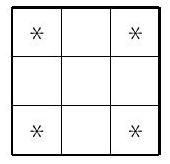
\includegraphics[max width=\textwidth, center]{2024_10_09_bce9f07034ef55fc9c97g-45}

图 4 - 4\\
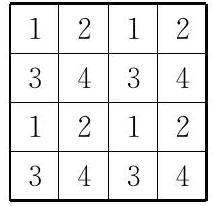
\includegraphics[max width=\textwidth, center]{2024_10_09_bce9f07034ef55fc9c97g-45(1)}

图 4 - 5

次, 恰好将 $4 \times 4$ 数表中的所有数的符号全部改变 (如图 $4-5$ 所示). 因此, 当 $4 \mid m$, 且 $4 \mid n$ 时, 可将 $m \times n$ 数表分成若干个互不相交的 $4 \times 4$ 数表, 并对每个 $4 \times 4$ 数表操作一次上述变换,可将 $m \times n$ 数表中的所有数的符号全部改变.

另一方面, 当 $m$ 与 $n$ 之一不是 4 的倍数时, 不能把数表中的所有数改变符号. 事实上, 不妨设 $4 \nmid m$. 选定方格表的一条长为 $m$ 的外框边, 并将靠这条边的一列称为第 1 列, 与第 1 列相邻的一列称为第 2 列. 用反证法, 假设可以通过一系列操作变换使表中所有数都变号. 如果将每个方格中的数在操作变换过程中符号变号的次数称为该方格的 "度",于是 $m \times n$ 的表格中每一个小方格的"度"都是奇数.\\
(1) 当 $m$ 为奇数时, 考察数表中第 1 列. 由于在每次操作变换中,第一列数要么全未变号, 要么两个方格变号, 从而第 1 列方格的度数之和为偶数, 通过一系列操作变换后仍是偶数. 由于 $m$ 为奇数, 故第 1 列中至少有 1 个方格的度数为偶数. 与假设相违, 结论成立.\\
(2)当 $m=4 k+2$, 其中 $k$ 为正整数, 由于每次涉及到第 1 列的操作恰好改变其中两个数的符号, 欲使 $(4 k+2)$ 个方格中的数全部变号, 涉及到第 1 列的变换必有奇数次. 在每一次这样的变换中, 第 2 列中都恰有 3 个数被改变符号; 而对那些不涉及第一列数的变换, 第二列中的数要么全未变号, 要么两个方格变号, 因此第 2 列中的数变号次数之和为奇数。但由于每个方格的度数均为奇数, 而方格数为偶数, 所以第 2 列方格的度数之和为偶数. 矛盾! 结论成立。

综上, 当且仅当 $m$ 和 $n$ 都是 4 的倍数, 题中要求可以实现.\\
例 8 给定 4 个全等的直角三角形纸片并允许进行如下操作: 每次可以选择一个直角三角形并将它沿斜边上的高剪开成两个直角三角形. 求证: 无论经过多少次操作, 在所得到的三角形中总有两个全等.

证明 用反证法. 即存在 4 个全等的直角三角形纸片, 经过有限次操作可使所得到的直角三角形互不全等。

设这样的有限次操作的最少次数为 $n$, 并考察达到 $n$ 次的这一组 4 个全等的直角三角形. 这里, 操作 $n$ 次可以使得到的直角三角形互不全等与先剪哪个直角三角形, 后剪哪个直角三角形的操作顺序无关.

开始时这 4 个是全等的直角三角形,故必须有 3 个全等直角三角形要沿斜边上的高剪开. 不妨设开头的 3 次操作就是前开这 3 个三角形. 于是得到新的 6 个直角三角形可以分成两组, 每组 3 个直角三角形彼此全等. 这样一来,每组 3 个全等直角三角形中又都至少剪开两个. 不妨设第 4 至第 7 次操作就是前开这 4 个三角形. 注意到, 这时剪开得到的 8 个直角三角形中有 4 个是全等的直角三角形 (相当于两个矩形沿它们的一条对角线剪开). 按假设, 从这 4个全等的直角三角形出发, 只要再操作 $(n-7)$ 次就可以得到互不全等的三角形,此时与 $n$ 的最小性矛盾! 这表明无论经过多少次操作, 总有两个三角形全等.

下面三个例子介绍多人游戏问题.\\
例 $9 n$ 个小朋友围成一圈,每人手中都有若干个球. 以下称为一次操作:若每个人都有偶数个球, 则每个人都分一半给右边的小朋友, 此时如果有小朋友手中有奇数个球, 则另外再给他 1 个球. 证明: 如果开始时每个小朋友手中球数均是偶数, 则若干次操作后, 每个人手中球数都相同了。

证明 设开始时最多有 $2 a$ 个球, 最少有 $2 b$ 个球. 若 $a=b$, 则已经全都相同了. 否则, 设有 $k$ 个人有 $2 b$ 个球, 则这 $k$ 个人中至少有一人在经过一次操作后球数 $>2 b$, 故至多 $k$ 次操作后, 最少球数 $\geqslant 2 b+2$, 而若手中有 $2 a$ 个球, 则经过一次操作后, 球数不会增加, 即最大数仍不大于 $2 a$, 从而经过有限次操作后, 最大数球数与最小数球数将相等, 从而每个人手中球数相同.

例10 甲、乙、丙三人做游戏. 共有三张牌, 其上分别写有正整数 $p 、 q 、 r$,且 $p<q<r$, 洗牌之后分发给三人, 每人一张, 并按每人所得牌上的数字付给弹子. 然后收牌再洗, 但所得的弹子由每人自己保存. 这样洗牌、发牌、付弹子的游戏至少进行两次。已知游戏结束时甲、乙、丙三人分别有弹子 20 个、 10 个和 9 个, 且乙最后一次得到 $r$ 个弹子。问谁在第一次游戏中得到 $q$ 个弹子?

解 设游戏次数为 $n$, 则\\
\begin{align*}
n(p+q+r)=20+10+9=39=3 \times 13
\end{align*}

由于 $0<p<q<r$, 故 $p+q+r \geqslant 6$. 又因 $n \geqslant 2$, 故 $n=3$, 且\\
\begin{align*}
p+q+r=13
\end{align*}

已知乙最后一次得到 $r$ 个弹子,因此另外两次得到的弹子数只能均为 $p$ (否则乙得到弹子数 $\geqslant 13$ )。由于丙得到的弹子总数少于乙得到的弹子总数,所以丙没有一次能得到 $r$ 个弹子。丙三次得到的弹子数为 $q, q, p$ 或 $q, q$ , $q$ ;又由于乙第 1 次得 $p$ 个弹子,故丙第 1 次得 $q$ 个弹子。

例 11 在圆桌上坐了 10 个人,在每人面前放一些糖果,共放了 100 粒糖果. 某个信号后,每个人将面前的糖果传给他右边的人,数额如下:若他有偶数粒糖果,则将一半给右边的人;若他有奇数粒糖果,则给右边的人的糖果数是他所有糖果数加 1 后的一半. 这个过程不断重复. 试证:最后每人面前都有 10 粒糖果.

证明 设在第 $j$ 次传递糖果时,第 $i$ 个人给出的糖果数为 $g_{i}(j)$ 粒,余下 $k_{i}(j)$ 粒糖果,其中 $1 \leqslant i \leqslant 10, j \geqslant 1$ 。因此,对任意 $i 、 j$,\\
\begin{align*}
0 \leqslant g_{i}(j)-k_{i}(j) \leqslant 1
\end{align*}

且\\
\begin{align*}
g_{i-1}(j)+k_{i}(j)=k_{i}(j+1)+g_{i}(j+1)
\end{align*}

这里约定 $g_{0}(j)=g_{10}(j), j$ 为任意正整数。由于\\
\begin{align*}
\left|g_{i}(j+1)-k_{i}(j+1)\right| \leqslant\left|g_{i-1}(j)-k_{i}(j)\right|
\end{align*}

则\\
\begin{align*}
\left[g_{i-1}(j)\right]^{2}+\left[k_{i}(j)\right]^{2} \geqslant\left[k_{i}(j+1)\right]^{2}+\left[g_{i}(j+1)\right]^{2}
\end{align*}

定义\\
\begin{align*}
s(j)=\sum_{i=1}^{10}\left\{\left[k_{i}(j)\right]^{2}+\left[g_{i}(j)\right]^{2}\right\}
\end{align*}

由(1)知 $s(j)$ 是关于 $j$ 的非增函数,且 $s(j)$ 是取整数值. 因此,一定存在 $t$ ,使 $s(t)$ 为它的最小值。这意味着当 $j \geqslant t, 1 \leqslant i \leqslant 10$ ,有\\
\begin{align*}
\left|g_{i-1}(j)-k_{i}(j)\right| \leqslant 1
\end{align*}

而且 $k_{1}(t), g_{1}(t), k_{2}(t), g_{2}(t), \cdots, k_{10}(t), g_{10}(t)$ 是相等的 20 个数字,即每个数都是 5 .

假设上述 20 个数中不全为 5 , 那么存在 $i 、 l$, 使得 $g_{i}(t)=6$ ,\\
\begin{align*}
k_{i+1}(t)=g_{i+1}(t)=\cdots=k_{l}(t)=g_{l}(t)=5
\end{align*}

并且 $k_{l+1}(t)=4$. 经过一次传递,可知 $g_{i+1}(t+1)=6$ ,\\
\begin{align*}
k_{i+2}(t+1)=g_{i+2}(t+1)=\cdots=k_{l}(t+1)=g_{l}(t+1)=5
\end{align*}

且\\
\begin{align*}
k_{l+1}(t+1)=4
\end{align*}

重复上述过程最后可得\\
\begin{align*}
\begin{gathered}
g_{l}(t+l-i)=6 \\
k_{l+1}(t+l-i)=4
\end{gathered}
\end{align*}

这与(2)矛盾!所以证明了这 20 个数都必须是 5 . 因此经过 $t$ 次传递后,每个人都有 10 粒糖果。

最后讨论两人游戏与博弈问题.\\
例12 有 100 个球,甲、乙二人依次从袋中拿球,每次可拿 1 个到 5 个,甲先拿,且拿到最后一个球的人为胜者,则最后的胜者是谁(假设两人都足够聪明)?

分析 要取得最后一个球,则在取到最后一个球前,当对手取球时,必须不少于 6 个。而如果多于 6 个,那么对手可以拿掉若干个,使球个数仍多于或等于 6 个,使得最后一次亦无法拿到最后一球,故胜者在最后拿球前让对手拿球时,球恰剩 6 个。依此向前推即可。

解 甲将获胜. 策略是:第一次取 4 球,以后若乙取 $k(1 \leqslant k \leqslant 5)$ 球,则甲取 6- $k$ 球,于是最后一轮必剩 6 球,无论乙取几球,甲都能取到最后一球。

例13 在 $n \times m$ ( $n 、 m$ 均大于 1 )的方格棋盘左下角有一棋子,甲、乙二人可以将棋子向右移若干格,也可以向上移若干格,谁不能再移动,谁就输了,问何时甲必胜,何时乙必胜?

分析 依题意可知,谁将棋子移到右上角,谁就赢了。当 $n=m$ 时,只要每两步操作都将棋子走在左下到右上的对角线上,那么后走者必是胜者。当 $n \neq$ $m$ ,那么第一步应使剩下能走的方格成正方形,这样,先走者必胜。

解 若 $n=m$ ,则甲必败。乙的必胜策略是:若甲向右(或向上)走 $k$ 格,则乙向上(或向右)走 $k$ 格,这样,甲、乙各走一次后,棋子沿对角线移动,故必是乙将它移到了右上角。

若 $m \neq n$ ,则甲必胜。甲的必胜策略是:先移动棋子,使棋子的右上方为正方形。这总是能办到的,要么是右移 $|m-n|$ 格,要么是上移 $|m-n|$ 格。于是,再应用 $n=m$ 时乙的策略知甲必胜。

例14 在 $n \times m$ ( $n 、 m$ 均大于 1 )的方格棋盘上,开始时所有格子均为白色,甲、乙二人轮流操作,甲先沿一条方格线将棋盘分成两个小棋盘,并将其

中一个小棋盘涂黑,然后乙在白色小棋盘上沿方格线将棋盘再分成两个小棋盘, 并将其中一个涂黑, 谁操作后只剩一个白色格子时为胜者, 问甲、乙谁必胜?

解 首先有一个事实:当棋盘为长方形时,必可操作一次,使剩下一个白色的正方形,而当棋盘为正方形时,操作一次后必为长方形。

所以, 若 $n \neq m$, 则甲必胜. 甲先将棋盘分成一个正方形和另一个图形 (可能是长方形也可能是正方形,然后剩下白色的正方形,这样,每次乙分完后剩下的都是长方形,而甲又可使分完后为正方形,从而最后剩下一格小正方形的必为甲。

而若 $n=m$, 则乙必胜. 策略是当甲完成第一步乙按上面甲的策略即可.\\
例 15 甲、乙两个人取数, 若已有的最后一个数为 $l$, 则可以取 $l+1$ 至 $2 l-1$ 中任一个数. 若甲先取, 开始已有数 2 , 取到 2004 为胜者, 则甲必胜还是乙必胜?

解 甲必胜. 甲可依次取3、7、15、31、62、125、250、501、1002、2004.\\
这一列数中, 后一个数要么是前一个数的 2 倍, 要么是 2 倍加上 1 . 现在说明只要取到前一个数, 就必可取到后一个数, 从而必可取到 2004.

事实上, 若甲取到的数为 $l$,则乙可取 $l+1$ 至 $2 l-1$ 中任一数. 而 $2(l+1)>2 l, 2(l+1)>2 l+1$ 且 $2 l>2 l-1,2 l+1>2 l-1$,故当乙取完后, 甲必可取 $2 l$ 或 $2 l+1$.

从而甲必胜。\\
例16 在正 $2 n$ 边形顶点相间染红、黑两色, 甲、乙两人轮流画上两端点同色的对角线,但不能与自己前面画的对角线相交,甲先画,不能画了就算输, 问甲必胜还是乙必胜?

解 乙必胜.\\
设正 $2 n$ 边形 $A_{1} A_{2} \cdots A_{2 n}$. 策略是: 当甲画对角线 $A_{i} A_{j}$ 时, 乙只须画对角线 $A_{i+1} A_{j+1}\left(A_{2 n+1}=A_{1}\right)$ 即可。

例 17 在 $10 \times 10$ 的棋盘上, 甲、乙两人做游戏. 操作是轮流进行的. 甲先往空格里填入 $\times$, 乙再往空格里填入 $\bigcirc$. 当所有 100 个格子都填满了时, 计算表格中两个特征数值 $C$ 和 $Z . C$ 是五个连续分布在一行、一列或一条斜率为 1的斜线上的 $\times$ 的组数, 如有六个这样的 $\times$, 就算 2 组, 有 7 个这样的 $\times$ 就算 3组, 如此等等. 类似地, $Z$ 是对 $\bigcirc$ 作同样的计算得出的. 如果 $C>Z$, 则甲胜; 如果 $C<Z$, 则甲败; 如果 $C=Z$, 则为平局. 问甲是否有策略足以保证: (1) 平局; (2) 得胜.

解 (1) 甲有成平局的策略. 从任何一个格子开始, 然后针对乙的走法,

关于一条能将棋盘分为两个 $10 \times 5$ 的轴线采取对称的动作. 如果乙画上一个对称于甲已画好的格子的格子,那么甲可画任何一个空格并重复这一过程.最后, 得到一个对称的图形, 保证了 $C=Z$.\\
(2) 甲没有必胜的策略. 由于乙可采用上述同样的对称策略,确保 $C=Z$.

例 18 某个游戏中第一个选手在平面上某点标以红色, 第二个选手在平面上未着色的点中取 10 点标以绿色. 接下去第一个选手和第二个选手轮流上述方法对未着色的点标上颜色. 如果有三个红点构成等边三角形, 则第一个选手胜. 是否第二个选手总能做到不让第一个选手胜?

解 第一个选手必胜.\\
因为在第 $n$ 步后, 第一个选手可在一条直线上取了 $n$ 个不同的红点, 相应地第二个选手作了 $10 n$ 个不同的绿点.

由于在直线一侧可以有 $\left(\mathrm{C}_{n}^{2}=\right) \frac{n(n-1)}{2}$ 个位置, 使这些位置打上红点,则和直线上某两点构成一个等边三角形. 因此在直线外有 $n(n-1)$ 个点, 只要在其中任一点标上红色就使第一个选手获胜。

由于第二个选手只能打上 $10 n$ 个绿点, 所以当 $n(n-1)>10 n$ 时, 第一个选手的第 $n+1$ 步必可得等边三角形. 由于 $n=12$ 时, 有\\
\begin{align*}
12(12-1)=132>120
\end{align*}

即到第 13 步,第一个选手必胜.\\
注 由于第一个选手可以避开第二个选手已标的绿点, 所以实际上在第 8 步即可获胜.

例19 甲、乙两人在黑板上玩写数的游戏, 规则是两人轮流在黑板上写一个不超过 $p$ 的自然数, 但禁止再写出黑板上已有数的因数. 甲先开始写, 轮到谁写而无法写出时就告负。\\
(1)当 $p=10$ 时, 游戏者中谁有获胜策略?\\
(2)当 $p=1000$ 时,游戏者中谁有获胜策略?\\
解 (1) 甲有获胜策略. 甲可以先写 6 , 于是按规则甲、 乙不能再写 1、2、 3. 把余下的 6 个数分成 3 组: $(4,5) 、(7,9) 、(8,10)$. 无论乙写哪一个, 甲就写同组的另一个,则甲可以获胜.\\
(2) 先考察一个写数原则相同但取数范围不是由 1 到 1000 , 而是由 2 到 1000 的游戏. 如果这个游戏先写者有必胜策略, 那么甲对原来游戏只要照搬就行了,这是由于甲写下一个正整数后,乙是不能写 1 的;如果这个新游戏先写数的人没有必胜策略, 即后写的人有必胜策略, 那么甲在原来游戏中可以先写 1 ,从而将失败留给了乙,即甲有必胜策略。总之,甲总有获胜策略。

例20 甲、乙两人轮流从共有 $n$ 块石头的石堆中取出石块。甲先开始,他第 1 次可以从堆中取走任意多块,但不能不取也不能全部取走。 以后每人每次所取石块数都应为对方刚才一次所取的石块数的约数,取得最后一块者胜。问对于怎样的最小的 $n>2005$ ,乙有获胜策略?

解 首先,我们断言,对 $n>1$ ,当且仅当 $n=2^{m}$ 时,乙有获胜策略。因而题中所求的最小的 $n=2048$.

设 $n=2^{m}$ ( $m$ 为正整数)。并设甲第 1 次所取的石块数为 $2^{m_{1}}\left(2 k_{1}+1\right)$ ,其中 $m_{1} 、 k_{1}$ 均为非负整数。于是乙只要按如下策略行事即可取胜:他第 1 次取走 $2^{m_{1}}$ 块,而在以后各次中,乙每次所取的块数都与甲刚刚所取走的块数相等。这样一来,甲在第 $h(h \geqslant 2)$ 次取石块时,所取的块数必为 2 的幂 $2^{m_{h}}$ 。于是必有 $0 \leqslant m_{h} \leqslant m_{h-1}$ ,并且甲取过之后,堆中所剩的石块数必为 $2^{m_{h}}$ 的奇数倍,当然不为 0 。因而最后获胜者必然是乙。

而对于 $n=2^{m}(2 k+1), k$ 为正整数。那么甲只要在第 1 次取走 $2^{m}$ 块,余下 $2^{m+1} k$ 块,这样,乙以后每次只能拿走 2 的一个指数不超过 $m$ 的方幂块石头,只要甲再采取前种情况乙的策略,现在乙每次余下的石块数都是 2 的幂的奇数倍,所以甲必胜,从而乙无必胜的策略。\\
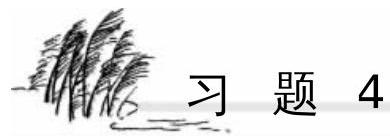
\includegraphics[max width=\textwidth, center]{2024_10_09_bce9f07034ef55fc9c97g-51}

1 是否存在这样的等腰三角形,它可以分成三个三角形,使得其中任意两个三角形可拼成一个新的等腰三角形。

2 在一个由 $n$ 个方格组成的 $1 \times n$ 棋盘中,每个方格上各放一枚钱币. 第一次搬动为将某一个方格上的钱币放在相邻的一个方格中的钱币上(在原来的方格的左边或右边都可以,但是不能出棋盘)。以后的每次搬动是将某个方格中的所有钱币(若有 $k$ 个)搬到与此方格相邻的第 $k$ 个位置的方格中。左或右都可以,但是不能出棋盘。试证:能经过 $(n-1)$ 次搬动,将所有钱币都集中在一个方格中。\\
3 已知一个圆周上写有若干个实数。如果对于其中依次相邻的 4 个数 $a 、 b$ 、 $c$ 、 $d$ ,有 $(a-d)(b-c)<0$ ,则可以交换 $b$ 和 $c$ 的位置。求证:这样的交换只能进行有限多次。\\
4 在黑板上写有三个数: $89 、 12 、 3$. 现进行如下操作:任取其中两个数,分别求其和与差并都除以 $\sqrt{2}$ ,然后用这两个数代替原来的两个数。问能否经过若干次操作使黑板上的三个数变为 $90 、 10 、 14$ ?说明理由。

5 国际象棋的一个车位于 $m \times n ( m 、 n$ 均大于 1$)$ 的棋盘的角格上. 两位游戏者轮流地在水平方向或坚直方向移动它,移动多少方格都行。车所经过的方格(包括通过的和停止的)都被涂上了颜色,车不能再经过或停止于已经涂色的格子。游戏者若无法再动,算输。谁有必胜的策略:先走的还是后走的?他该如何动作?\\
6 现有一个正方体和两种颜色:红色和绿色。甲、乙两人做如下的游戏:甲先取正方体的三条棱,并将它们涂上红色;乙从尚未涂色的棱中选三条并将它们涂上绿色;然后甲再从尚未涂色的六条棱中选三条并涂上红色;最后乙将剩下的三条涂成绿色。谁能首先把一面的四条棱涂成同一种颜色,谁就获胜。问:甲是否有必胜策略。\\
7 甲、乙两人轮流在 $25 \times 25$ 的方格棋盘上放置棋子,甲执白先下,乙执黑,每颗新子都放于空格之中,但若一个空格的 4 个邻格(即有公共边的方格称为邻格)都已被同色棋子占领,则禁止在其中再放此种颜色的棋子。若轮到某人着棋时无处下子,则此人告负。问当谁采用正确策略时,必能获胜?\\
8 黑板上写有 2005 个数 $1,2 , \cdots , 2^{2004}$ 。甲、乙两人轮流在这些数中挑 5 个数各减去 1 ,若某个人在操作后有负数,则此人为败。若甲先操作,问谁将获胜?\\
9 某校数学小组的学生做成一种计算器,按下按钮即可将数组 $(a, b, c, d)$变成数组 $(a-b, b-c, c-d, d-a)$ 。试证:如果开始的四个数不全相等,那么按若干次按钮后得到的数组中至少有一个数的绝对值大于 2005.\\
10 正五边形的每个顶点对应一个整数,使得这五个整数的和为正数。若其中三个相邻顶点对应的整数依次为 $x 、 y 、 z ,$ 而中间的 $y<0$ ,则要进行如下的变换:整数 $x 、 y 、 z$ 分别换为 $x+y 、-y 、 z+y$ 。要是所得的五个整数中至少还有一个为负数,这种变换就继续进行。问:这样的交换进行有限次后是否必定终止?\\
11 将 $2^{n}(n \geqslant 1)$ 个数排在一个圆周上,每个数都是 +1 或 -1 ,现在同时将每个数都乘以它的右边的数,将所得到的数替换原来的数,称为一次操作。证明:经过有限次操作后,每个数都成为 +1 。

\section{组合最值}
组合最值问题是离散变量最值问题中的一种重要题型,通常分为组合最大值和组合最小值两类问题。

一个变量随着一组对象的安排方式不同而变化,适当地安排这组对象,可使变量的相应的值取到最大或最小,通常称其为组合最值问题。从问题结构上来说,解组合最值问题包括两个方面:一方面,变量的最大值或最小值是多少;另一方面,如何具体安排对象,使变量达到最值。针对这两方面,解决组合最值问题,通常有以下两个步骤:\\
(1)估计:即对变量的值作出估计,准确地找到变量的上界或下界。\\
(2)构造:即构造一种具体的安排方式,以证明第一步估计的上界或下界能取到.

我们以下从组合最大值和组合最小值两类题型给出实例分析,突出组合估计与组合构造的解题技巧。

例1 求最大的正整数 $n$ ,使得 $n$ 为集合 $S$ 中元素的个数,且满足:\\
(1) $S$ 中的每个数均为不超过 2004 的正整数;\\
(2)对于 $S$ 中的两个数 $a 、 b$ (可以相同),它们的积 $a b$ 不属于集合 $S$ 。\\
解 一方面,取集合 $S=\{45,46,47, \cdots, 2004\}$ ,此时该集合中任意两个数(可以相同)的积最小值是 $45^{2}=2025>2004$ 。因此,集合 $S$ 满足条件, $S$中元素的个数为 1960 。

另一方面,考察 $A_{1}=\{1\} , A_{2}=\{2,87,2 \times 87\}, A_{3}=\{3,86,3 \times 86\} ,$ $A_{4}=\{4,85,4 \times 85\}, \cdots, A_{43}=\{43,46,43 \times 46\}, A_{44}=\{44,45,44 \times 45\}$等 44 个集合,易知其中每一个集合中至少去掉一个元素(否则,其中两个数之积仍在该集合中)。因此,从 1 至 2004 中至少去掉 44 个数,即构成集合 $S$ 的元素不超过( $2004-44=) 1960$ 个。

综合两方面可知: $n$ 的最大值为 1960 。\\
例 2 在一个有限项的实数数列中,任何 3 个连续项之和都是负数,而且任何 4 个连续项的和为正数, 求此数列项数的最大值 $r$.

解 $r$ 的最大值为 5 .\\
一方面, 构造一个 5 项的数列: $2,2,-5,2,2$, 其中任何 3 个连续项之和为 -1 , 任何 4 个连续项之和为 1 . 因此 $r=5$ 时, 存在满足题设的由 5 项组成的数列。

另一方面, 证明满足条件的任意有限项 ( $r$ 项) 的实数列, 则 $r \leqslant 5$. 用反证法.

假设 $r \geqslant 6$, 我们取出此数列的前 6 项, 并作如下 $4 \times 3$ 的表格排列:\\
\begin{align*}
\begin{aligned}
& a_{1}, a_{2}, a_{3} \\
& a_{2}, a_{3}, a_{4} \\
& a_{3}, a_{4}, a_{5} \\
& a_{4}, a_{5}, a_{6}
\end{aligned}
\end{align*}

上述表中每一行是数列连续 3 项之和,每一列是数列连续 4 项之和,由已知条件, 则该表中每一行之和均小于 0 ,而每一列之和大于 0 。

考虑计算该表中所有数的和 $M$ (即 $a_{1}+2 a_{2}+3 a_{3}+3 a_{4}+2 a_{5}+a_{6}$ )。依各行考虑, 每行和小于 0 , 得\\
\begin{align*}
M<0
\end{align*}

依各列考虑, 每列和大于 0 , 得\\
\begin{align*}
M>0
\end{align*}\\
(1)与(2)矛盾!所以假设不成立,故 $r \leqslant 5$ 。

例3 已知 $b, c$ 为给定的两个实数, 问最多能有多少个不同的整数 $x$, 满足 $\left|101 x^{2}+b x+c\right| \leqslant 50$.

解 一方面, 取 $b=c=-50$, 记\\
\begin{align*}
f(x)=101 x^{2}+b x+c=101 x^{2}-50 x-50
\end{align*}

则\\
\begin{align*}
\begin{aligned}
& |f(0)|=|-50| \leqslant 50 \\
& |f(1)|=|1| \leqslant 50
\end{aligned}
\end{align*}

因此, 存在这样的实数 $b 、 c$, 使得有两个不同的整数 $x$, 满足\\
\begin{align*}
\left|101 x^{2}+b x+c\right| \leqslant 50
\end{align*}

另一方面, 无论 $b 、 c$ 是怎样给定实数, 至多存在两个不同的整数 $x$, 满足\\
\begin{align*}
\left|101 x^{2}+b x+c\right| \leqslant 50
\end{align*}

用反证法, 假设存在三个不同的整数 $x_{1} 、 x_{2} 、 x_{3}$ 满足\\
\begin{align*}
\left|101 x^{2}+b x+c\right| \leqslant 50
\end{align*}

由抽屉原理知: $x_{1} 、 x_{2} 、 x_{3}$ 中必有两个数同时大于或等于 $-\frac{b}{2 a}=-\frac{b}{202}$ (或者两个数同时小于或等于 $-\frac{b}{2 a}$ ,这种情况可类似于前者的证明),不妨设\\
\begin{align*}
x_{1}>x_{2} \geqslant-\frac{b}{2 a}=-\frac{b}{202}
\end{align*}

利用不等式 $|x-y| \leqslant|x|+|y|$ 知,\\
\begin{align*}
\begin{aligned}
\left|f\left(x_{1}\right)-f\left(x_{2}\right)\right| & \leqslant\left|f\left(x_{1}\right)\right|+\left|f\left(x_{2}\right)\right| \\
& =\left|101 x_{1}^{2}+b x_{1}+c\right|+\left|101 x_{2}^{2}+b x_{2}+c\right| \\
& \leqslant 50+50=100
\end{aligned}
\end{align*}

而\\
\begin{align*}
\begin{aligned}
\left|f\left(x_{1}\right)-f\left(x_{2}\right)\right| & =\left|101 x_{1}^{2}+b x_{1}+c-101 x_{2}^{2}-b x_{2}-c\right| \\
& =\left|\left(x_{1}-x_{2}\right)\left[101\left(x_{1}+x_{2}\right)+b\right]\right|,
\end{aligned}
\end{align*}

又由于\\
\begin{align*}
x_{1}-x_{2} \geqslant 1
\end{align*}\\
\begin{align*}
\begin{aligned}
101\left(x_{1}+x_{2}\right)+b & \geqslant 101\left[\left(x_{2}+1\right)+x_{2}\right]+b=101+202 x_{2}+b \\
& \geqslant 101+202 \cdot\left(-\frac{b}{202}\right)+b=101
\end{aligned}
\end{align*}

故\\
\begin{align*}
\begin{aligned}
\left|f\left(x_{1}\right)-f\left(x_{2}\right)\right| & =\left|x_{1}-x_{2}\right| \cdot\left|101\left(x_{1}+x_{2}\right)+b\right| \\
& \geqslant\left|101\left(x_{1}+x_{2}\right)+b\right| \\
& \geqslant 101>100
\end{aligned}
\end{align*}

比较(1)与(2), 两个不等式矛盾!\\
故假设不成立,即结论成立。\\
综合这两方面, 最多有两个不同的整数 $x$, 满足 $\left|101 x^{2}+b x+c\right| \leqslant 50$.\\
例 4 已知 $A 、 B$ 是由有限个不同的正实数组成的两个集合, 集合 $A$ 和 $B$都至少含有 3 个元素。若集合 $A$ 中任意 3 个不同实数的和均在集合 $B$ 中,集合 $B$ 中任意 3 个不同实数的积均在集合 $A$ 中. 求 $A$ 和 $B$ 的元素个数和的最大值。

解 一方面,取集合 $A=\{1,2,3\}$,集合 $B=\left\{\frac{1}{6}, 1,6\right\}$ 满足条件,此时集合 $A 、 B$ 均有 3 个元素, 元素的个数和为 6 .

另一方面,先证明集合 $A$ 中恰好含有 3 个元素。

用反证法,假设 $A$ 中恰含有 $m(m \geqslant 4)$ 个元素,设为 $a_{1}, a_{2}, \cdots, a_{m}$ ,且 $0<a_{1}<a_{2}<\cdots<a_{m}$ 。记\\
\begin{align*}
\begin{gathered}
S=a_{1}+a_{2}+a_{3}+a_{4} \\
P=\left(S-a_{1}\right)\left(S-a_{2}\right)\left(S-a_{3}\right)\left(S-a_{4}\right)
\end{gathered}
\end{align*}

由已知条件知 $S-a_{1}, S-a_{2}, S-a_{3}, S-a_{4}$ 均属于集合 $B$.\\
当 $m \geqslant 5$ 时,易知 $\alpha_{1}=\frac{P}{S-a_{1}}, \alpha_{2}=\frac{P}{S-a_{2}}, \alpha_{3}=\frac{P}{S-a_{3}}, \alpha_{4}=\frac{P}{S-a_{4}}$, $\alpha_{k}=\frac{P\left(S-a_{1}-a_{4}+a_{k}\right)}{\left(S-a_{3}\right)\left(S-a_{4}\right)}(k=5, \cdots, m), \alpha_{m+1}=\frac{P\left(S-a_{1}-a_{3}+a_{m}\right)}{\left(S-a_{3}\right)\left(S-a_{4}\right)}$ 均为 $B$ 中的 3 个不同元素的积(这里 $S-a_{1}-a_{4}+a_{k}(k=5, \cdots, m), S-a_{1}-a_{3}+$ $a_{m}$ 均属于集合 $B$ ),因此均在 $A$ 中。

由于 $S-a_{1}>S-a_{2}>S-a_{3}>S-a_{4}>0$ ,故 $0<\alpha_{1}<\alpha_{2}<\alpha_{3}<\alpha_{4}$ ;\\
由于 $a_{1}<a_{3}, a_{4}<a_{5}$, 所以 $S-a_{1}-a_{4}+a_{5}>S-a_{3}$, 从而\\
\begin{align*}
\alpha_{4}=\frac{P}{S-a_{4}}<\frac{P\left(S-a_{1}-a_{4}+a_{5}\right)}{\left(S-a_{3}\right)\left(S-a_{4}\right)}=\alpha_{5} ;
\end{align*}

由于 $a_{i}<a_{i+1}(i=5, \cdots, m-1)$ ,故\\
\begin{align*}
\frac{P\left(S-a_{1}-a_{4}+a_{i}\right)}{\left(S-a_{3}\right)\left(S-a_{4}\right)}<\frac{P\left(S-a_{1}-a_{4}+a_{i+1}\right)}{\left(S-a_{3}\right)\left(S-a_{4}\right)}
\end{align*}

即 $\alpha_{i}<\alpha_{i+1}(i=5, \cdots, m-1) ;$\\
由于\\
\begin{align*}
\frac{P\left(S-a_{1}-a_{4}+a_{m}\right)}{\left(S-a_{3}\right)\left(S-a_{4}\right)}<\frac{P\left(S-a_{1}-a_{3}+a_{m}\right)}{\left(S-a_{3}\right)\left(S-a_{4}\right)}
\end{align*}

故 $\alpha_{m}<\alpha_{m+1}$.\\
综上,有 $0<\alpha_{1}<\alpha_{2}<\cdots<\alpha_{m}<\alpha_{m+1}$ 。因此集合 $A$ 中至少含有 $m+1$ 个不同元素,与假设矛盾!

当 $m=4$ 时,同上讨论可知 $\alpha_{1}<\alpha_{2}<\alpha_{3}<\alpha_{4}$ ,这 4 个数正好是 $A=\left\{a_{1} ,\right.$ $\left.a_{2}, a_{3}, a_{4}\right\}$ 中的 4 个数,则 $a_{i}=\frac{P}{S-a_{i}}(i=1,2,3,4)$ ,即 $a_{i}^{2}-S a_{i}+P=$ 0. 因此,关于 $x$ 的一元二次方程 $x^{2}-S x+P=0$ 有四个不同实根 $a_{1} 、 a_{2} 、 a_{3}$ 、 $a_{4}$ 。这是不可能的。因此,集合 $A$ 中恰有 4 个元素也是不成立的。

因此,集合 $A$ 中恰含有 3 个不同元素。\\
再证明:集合 $B$ 中恰含有 3 个不同元素。用反证法,假设 $B$ 中含有 4 个以上不同元素,设其中 4 个元素为 $b_{1} 、 b_{2} 、 b_{3} 、 b_{4}$ ,不妨设 $0<b_{1}<b_{2}<b_{3}<b_{4}$ ,

则\\
\begin{align*}
0<b_{1} b_{2} b_{3}<b_{1} b_{2} b_{4}<b_{1} b_{3} b_{4}<b_{2} b_{3} b_{4}
\end{align*}

且 $b_{1} b_{2} b_{3} 、 b_{1} b_{2} b_{4} 、 b_{1} b_{3} b_{4} 、 b_{2} b_{3} b_{4}$ 是 $B$ 中 3 个不同元素的积,当然均在 $A$ 中。这与前面已证:集合 $A$ 中恰含有 3 个不同元素,矛盾!所以集合 $B$ 中亦恰含有 3 个不同元素。

总之,集合 $A$ 和 $B$ 中均恰有 3 个元素,元素的个数和的最大值为 6.\\
例 5 已知 $N$ 支排球队参加比赛,每支球队与其他任一支球队只比赛 1场。一支球队获胜积 1 分,失败记 0 分(排球比赛没有平局)。若任意 4 支球队之间进行的比赛中,至少有两个球队积分相同。求 $N$ 的最大值。

解 先证明:每支球队最多胜了 3 场比赛。\\
用反证法,假设球队 $A$ 至少胜了 4 场,不妨设 $A$ 胜了 $B 、 C 、 D 、 E$ 四支队. 考虑 $B 、 C 、 D 、 E$ 中的 3 支球队,如 $B 、 C 、 D$ ,由于 $A 、 B 、 C 、 D$ 四支球队中共有 6 场比赛,而 $A$ 已胜 3 场积 3 分,剩下的 3 分只好 $B 、 C 、 D$ 各积 1 分 (因为任意四支球队之间的比赛中,至少有两个球队积分相同),即在 $B 、 C 、 D$三支球队之间,每队各胜 1 场。同理 $B 、 C 、 E$ 三支球队之间,每队各胜 1 场, $C 、 D 、 E$ 三支球队之间,每队也各胜 1 场。但这是不可能的。故假设不成立,结论成立.

再次, $N$ 支球队 的循环赛中所有球队得分总和等于比赛场数,即 $\frac{N(N-1)}{2}$. 而每支球队得分不超过 3 分,得分总和不超过 $3 N$ 。因此, $\frac{N(N-1)}{2} \leqslant 3 N$ ,解得 $N \leqslant 7$ 。

下面构造 7 支球队 $A 、 B 、 C 、 D 、 E 、 F 、 G$的得分表,如图5-1。若 $A$ 胜 $B$ ,则在 $A$ 队所在行及 $B$ 队所在列处记 1 ,否则记为 0 ,其余类似,该表中某队的得分是该队所在行的 6 个元素之和。直接验证与任意四个队的比赛对应的一个 $4 \times 4$ 的方阵(共有 35 个不同的 $4 \times 4$ 方阵)中总存在两行的和相等,即至少有两个队的积分相同。

图5-1\\
故 $N$ 的最大值为 7 。\\
例 6 把棋子放在 $8 \times 8$ 的国际象棋棋盘的方格上,每格至多放 1 枚棋子,要求在每一行、每一列以及每一斜线上都刚好有偶数枚棋子,试问最多可以放置多少枚棋子?

解 最多可以放 48 枚棋子.\\
一方面, 如图 $5-2$, 在 $8 \times 8$ 的国际象棋盘上恰有 16 条对角线 (用虚线表示), 每条对角线包含奇数个小方格, 且任意两条对角线上的小方格没有公共方格. 从而要保证每条斜线上有偶数枚棋子,至少有 16 个方格不放棋子, 即最多只能放 48 枚棋子。

另一方面, 可以放 48 枚棋子, 使得每一行、每一列以及每一斜线上都刚好有偶数枚棋子。构造如下:

图5-2\\
只要在两条主对角线上的 16 个小方格中不放棋子,其他每一个方格上各放上 1 枚棋子。

例 7 从规格为 $2 n \times 2 n$ 的正方形中最多能剪出多少个规格为 $1 \times(n+1)$的矩形?

解 当 $n=1$ 时,最多可剪出 2 个 $1 \times 2$ 的矩形。\\
当 $n=2$ 时, 最多可剪出 5 个 $1 \times 3$ 的矩形.\\
当 $n=3$ 时,最多可剪出 8 个规格为 $1 \times 4$ 的矩形。\\
事实上, 一方面, 易知可剪出 8 个规格为 $1 \times 4$ 的矩形. 另一方面, 最多能剪出 8 个矩形, 将 $6 \times 6$ 的正方形方格分成 36 个小方格, 并把 $1 、 2 、 3 、 4 、 1 、 2$填入第一行, 第二行轮换填入 $2 、 3 、 4 、 1 、 2 、 3$, 依次类推, 如图 $5-3$. 剪出的任何一个 $1 \times 4$ 的矩形中都恰好含有数字 $1 、 2 、 3 、 4$. 而表中共有 9 个 $1 、 10$个 $2 、 9$ 个 $3 、 8$ 个 4 ,故最多能剪出 8 个规格为 $1 \times 4$ 的矩形。

\begin{center}
\begin{tabular}{|l|l|l|l|l|l|}
\hline
1 & 2 & 3 & 4 & 1 & 2 \\
\hline
2 & 3 & 4 & 1 & 2 & 3 \\
\hline
3 & 4 & 1 & 2 & 3 & 4 \\
\hline
4 & 1 & 2 & 3 & 4 & 1 \\
\hline
1 & 2 & 3 & 4 & 1 & 2 \\
\hline
2 & 3 & 4 & 1 & 2 & 3 \\
\hline
\end{tabular}
\end{center}

图5-3

图5-4

当 $n \geqslant 4$ 时,最多可剪出 $4(n-1)$ 个规格为 $1 \times(n+1)$ 的矩形.\\
事实上, 一方面, 可在 $2 n \times 2 n$ 的正方形中左上角先剪出规格为 $(n+1) \times$ 1 的 $(n-1)$ 个矩形, 再依次在右上角、左下角、右下角可剪出规格为 $1 \times(n+1)$的 $(n-1)$ 个矩形、 $1 \times(n+1)$ 的 $(n-1)$ 个矩形、 $(n+1) \times 1$ 的 $(n-1)$ 个矩形, 如图5-4. 中间余下一个边长为 2 的正方形, 面积为 4 . 因此, 总共剪出 $4(n-$

1)个规格为 $1 \times(n+1)$ 的矩形。另一方面,由 $4 n^{2}=4(n-1)(n+1)+4$ ,余下的面积为 4 ,不够剪出一个规格为 $1 \times(n+1)$ (因 $n \geqslant 4$ ,有 $n+1 \geqslant 5$ )的矩形。

综上可知,当 $n=1$ 时,最多可剪出 2 个矩形;当 $n=2$ 时,最多可剪出 5 个矩形;当 $n \geqslant 3$ 时,最多可剪出 $4(n-1)$ 个矩形。

例 8 用水平和坚直的直线网把一块正方形黑板分成边长为 1 的 $n^{2}$ 个小方格。试问:对怎样的最大正整数 $n$ ,一定可以选出 $n$ 个小方格,使得任意面积不小于 $n$ 的矩形中都至少包含上面选出的一个小方格(矩形的边都在网格线上)?

解 $n$ 的最大值为 7 。\\
一方面,当 $n=7$ 时,可以在 $7 \times 7$ 的网格中选取 7 个小方格(在图中标记为"○"),使得任意面积 $\geqslant 7$的矩形中都至少包含一个标记为"○"的小方格,具体构造如图 $5-5$ ,直接验证可知结论成立。

另一方面,证明 $n \leqslant 7$ 。用反证法,假设 $n>7$ 。如果选出 $n$ 个小方格满足问题的条件,那么在每一行和每一列都恰有一个选定的小方格。因此,先取定一\\
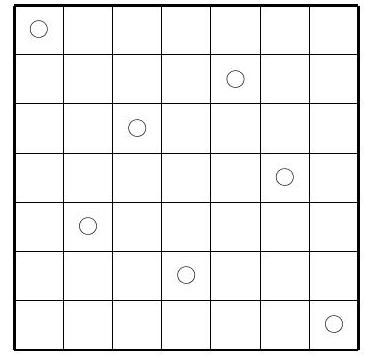
\includegraphics[max width=\textwidth, center]{2024_10_09_bce9f07034ef55fc9c97g-59}

图5-5

行(记为 $A$ 行),该行第一个小方格是选定的。又取和 $A$ 行相邻的为 $B$ 行。再取 $C$ 行,它或是与 $A$ 行相邻但不与 $B$ 行重合,或是与 $B$ 行相邻但不与 $A$ 行重合。

假设 $b$ 是 $B$ 行中的选定方格的位置(即该行中第 $b$ 个小方格是选定的)。\\
若 $b \leqslant n-\left[\frac{n+1}{2}\right]$ ,则在 $A$ 与 $B$ 两行中后面的 $\left[\frac{n+1}{2}\right]$ 个小方格都不是选定的,因此这相邻两行有一个面积为 $2 \times\left(\left[\frac{n+1}{2}\right]\right) \geqslant n$ 的矩形,它不含选定的小方格. 矛盾!

若 $b \geqslant\left[\frac{n+1}{2}\right]+2$, 则在 $A$ 行与 $B$ 行的第 1 格到第 $b$ 格之间都不含选定的小方格,因此也有一个面积为 $2 \times\left(\left[\frac{n+1}{2}\right]\right) \geqslant n$ 的矩形不含选定的小方格. 亦矛盾!

因此,有 $n-\left[\frac{n+1}{2}\right]<b<\left[\frac{n+1}{2}\right]+2$ (由于 $\left[\frac{n+1}{2}\right]+2>n-$ $\left[\frac{n+1}{2}\right]+1$, 所以这样的 $b$ 是存在的).

现在考虑 $A 、 B 、 C$ 三行的第 $2,3, \cdots, n-\left[\frac{n+1}{2}\right]$ 列,以及第 $\left[\frac{n+1}{2}\right]+$\\
$2,\left[\frac{n+1}{2}\right]+3, \cdots, n$ 列所构成的两个矩形,它们的面积都是\\
\begin{align*}
S=3 \times\left(n-\left[\frac{n+1}{2}\right]-1\right)
\end{align*}

而且这两个矩形中都不含有 $A 、 B$ 两行中已选定的小方格。\\
由于 $n>7$ ,易证\\
\begin{align*}
S=3\left(n-\left[\frac{n+1}{2}\right]-1\right) \geqslant n
\end{align*}

而 $C$ 行中只有一个选定的小方格,由抽屉原理知,上述两个矩形中必定有一个不含有选定的小方格,且该矩形的面积 $\geqslant n$ 。与题设相违!假设不成立,因而 $n \leqslant 7$ 。

例 9 已知一个 $10 \times 10 \times 10$ 的立方体网格,甲、乙、丙三个人按如下规则做游戏:他们以甲、乙、丙的次序轮流进行,分别从三个不同的方向将 $1 \times 1 \times$ 10 的砖形物放入立方体网格内,每个人有一个固定方向放置砖形物。砖形物应该全部放入已知的立方体网格内。问该游戏最多进行多少轮?(每一轮是指甲、乙、丙各放一次砖形物)

解 游戏最多进行 25 轮。\\
不妨设甲只能将 $1 \times 1 \times 10$ 的砖形物前后方向摆放,乙只能将 $1 \times 1 \times 10$ 的砖形物上下(坚直)方向摆放,丙只能将 $1 \times 1 \times 10$ 的砖形物左右(横向)方向摆放。

一方面,将 $10 \times 10 \times 10$ 的立方体网格分成 8 个相同的 $5 \times 5 \times 5$ 的立方体格,如图5-6. 甲的 25 个砖形物全部放入长方体 $A B H G-A_{1} B_{1} H_{1} G_{1}$ ,乙的 25 个砖形物全部放入长方体 $B C F E-B_{2} C_{2} F_{2} E_{2}$ ,丙的 25 个砖形物全部放入长方体 $D_{1} F_{1} I_{1} G_{1}-D_{2} F_{2} I_{2} G_{2}$ 。因此,该游戏可以进行 25 轮。

图5-6\\
图 5 - 7\\
另一方面,该游戏不能多于 25 轮。用反证法,假设游戏进行了 $m(m>$ 25)轮。因为 $m>5^{2}$ ,故在面 $A C C_{2} A_{2}$ 上至少有 6 行(或 6 列)中有甲放入的砖形物. 不妨设是靠近右侧的 6 列中有甲放入的砖形物(如图5-7)。

这样,乙放置的 $m$ 个砖形物全坚直方向地分布在长方体 $A J K G-$ $A_{2} J_{2} K_{2} G_{2}$ ,其中 $A J \leqslant 4$ ,则 $\frac{m}{A J}>6$ ,故由平均数原理,在面 $A J J_{2} A_{2}$ 上必有一个垂直于该面的 $1 \times 10$ 的方格条,其中至少有 7 个方格乙已放入砖形物。

同理,丙放置的砖形物全在一个 $3 \times 10 \times 10$ 的长方体 $L M I G-L_{2} M_{2} I_{2} G_{2}$内. 因为 $\frac{m}{3}>8$ ,则可推知甲放置的砖形物全在一个 $1 \times 10 \times 10$ 的长方体 $A^{\prime} C^{\prime} I^{\prime} G^{\prime}-A_{2} C_{2} I_{2} G_{2}$ 内。这显然矛盾!故 $m \leqslant 25$ 。最小性证毕。

例10 试求最大的正整数 $N$ ,使得无论怎样将正整数 1 至 400 填入 $20 \times$ 20 方格表的各个格中,都能在某一行或某一列中找到两个数,它们的差不小于 $N$ 。

\section{解 $N$ 的最大值是 209 .}
一方面,证明 $N \leqslant 209$ 。构造如下:\\
如图5-8,用 $A B$ 与 $C D$ 的中点 $E 、 F$ 连线分方格表为两个 20 行 10 列的方格表。将 1 至 200 逐行依递增顺序填入左表(即 $20 \times 10$ 的方格 DFEA)中,将 201 至 400 逐行依递增顺序填入右表(即 $20 \times 10$ 的方格 $F C B E$ )中。此时,每一行中所填入的数的最大差为 $210-1=209$ ,在每一列中所填入的数的最大差为 $191-1=190$ 。因此, $N \leqslant 209$ 。

另一方面,证明 $N=209$ 。即证:无论怎样将正整数 1 至 400 填入 $20 \times 20$方格表的各个格中,都能在某一行或某一列中找到两个数,它们的差 $\geqslant 209$ 。

考虑两个集合 $M_{1}=\{1,2, \cdots, 91\}$ ,及 $M_{2}=\{300,301, \cdots, 400\}$ 。将凡是填有 $M_{1}$ 中的数所在行和列都染为红色,将凡是填有 $M_{2}$ 中的数所在行和列都染为蓝色。

在 $20 \times 20$ 的方格表中,设有 $i$ 行和 $j$ 列被染为红色。由于 $M_{1}$ 中的 91 个元素全都位于这些行与这些列的相交处,故 $i j \geqslant 91$ 。

由于 $(\sqrt{i}-\sqrt{j})^{2} \geqslant 0$ ,所以\\
\begin{align*}
i+j \geqslant 2 \sqrt{i j} \geqslant 2 \sqrt{91}>19
\end{align*}

因此\\
\begin{align*}
i+j \geqslant 20
\end{align*}

设有 $k$ 行和 $l$ 列被染为蓝色,类似地有 $k l \geqslant 101$ ,故\\
\begin{align*}
k+l \geqslant 2 \sqrt{k l} \geqslant 2 \sqrt{101}>20
\end{align*}

即\\
\begin{align*}
k+l \geqslant 21
\end{align*}

由(1)、(2)知,在该方格表中染红色的行和列的数目 $\geqslant 20$ ,染蓝色的行和列的数目 $\geqslant 21$ ,而该方格表行和列的数目共计 40 。由抽屉原理知,必存在某一行或某一列既被染为红色,又被染为蓝色,从而其中必有两个数的差 $\geqslant 300-$ $91=209$.

例11 7 名学生参加校园科技节,学校准备给他们安排 $m$ 次活动展示,每次由其中 3 位学生展示各自科技成果。请你给学校设计一种方案,使得 7 名学生中任意两位同时展示的次数都一样多,且科技活动展示的次数 $m$ 最小。

分析 首先确定 $m$ 的范围,再构造满足学校要求的最小 $m$ 的方案。\\
解 设任意两位学生都同时展示的次数为 $r$ 。\\
7 名学生中任意两位学生的对子有 $\left(\mathrm{C}_{7}^{2}=\right) 21$ 个,每个对子都同时展示的次数为 $r$ ,因此任意两位学生的对子同时展示的总次数为 $21 r$ 。

每次活动由 3 位学生展示,两位学生的对子有 3 对,学校准备安排 $m$ 次科技活动展示,因此两位学生的对子同时展示的总次数为 3 m 。故满足学校设计方案的要求,须有 $3 m=21 r$ ,即 $m=7 r$ 。

易知 $r \geqslant 1$ ,从而 $m \geqslant 7$ 。\\
下面设计一种方案说明 $m=7$ 符合要求. 设 7 名学生编号 $1,2, \cdots, 7$.安排:

第一次活动由学生 1、2、3 展示;\\
第二次活动由学生 3、4、5 展示;\\
第三次活动由学生 1、4、7展示;\\
第四次活动由学生 2、4、6展示;\\
第五次活动由学生 3、6、7展示;\\
第六次活动由学生 2、5、7展示;\\
第七次活动由学生 $1 、 5 、 6$ 展示。\\
经验证, 7 名学生中任意两位同时展示的次数恰好都是一次。\\
例12 $6 \times 6$ 的棋盘中至少要放多少个马,才能保证控制整个棋盘(即控制所有空格和保护到所有已占格子的马)?(马的走法是国际象棋规则)

解 如图5-9,8个马可以控制所有空格,且保护到所有已占格子的马.

下面证明:在 $6 \times 6$ 的棋盘中至少要放 8 个马。\\
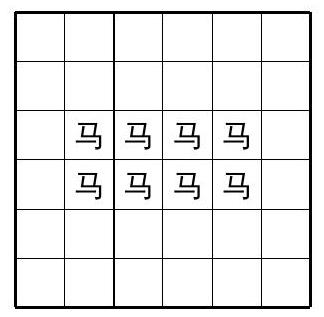
\includegraphics[max width=\textwidth, center]{2024_10_09_bce9f07034ef55fc9c97g-62}

图5-9

如图5-10,将棋盘相间地黑白染色,阴影部分表黑格,空白表白格。将每行每列标上1、2、3、4、 $5 、 6$ ,每个格子对应一个坐标 $(i, j)$ ,其中 $i, j=1$ , $2, \cdots, 6$. 记放在黑格中的马为黑格马,放在白格中的马为白格马。先证白格马至少 4 个。

黑格 $(1,1) 、(2,2) 、(6,6)$ 三个格子中任意两个格子不能同时由一个白格马控制,故至少须有 3 个白格马。假设只有 3 个白格马。控制(5,5)的白

图 5 - 10

格马必同时能控制(2,2),因此必有且只有一个白格马在(3,4)或(4,3)内。若 $(3,4)$ 有马,(4,3)无马。因(5,1)要受控制,而白格马(3,4)和控制(6,6)的马均不能控制 $(5,1)$ ,故只能由控制 $(1,1)$ 的马来控制它,即有白格马(3, 2 )。但白格马 $(3,2) 、(3,4)$ 及控制 $(6,6)$ 的马都不能控制 $(3,1)$ 。因此,此时仅有 3 个白格马不能控制所有的黑格。若(4,3)有马,(3,4)无马,类似的讨论可知仅有 3 个白格马不能控制所有的黑格。总之,白格马至少 4 个.

其次,同样地,证明黑格马至少 4 个. 故在 $6 \times 6$ 的棋盘中至少放 4 个白格马和 4 个黑格马,共计 8 个马。

综上所述,能控制 $6 \times 6$ 的棋盘所有空格和保护到所有已占格子的马最小值为 8 .

例 13 将正九边形的 5 个顶点涂上红色,问最少存在多少对全等三角形,它们的顶点都是红点?

解 全等三角形的最小对数有 4 对。\\
一方面, 设 $A_{1} 、 A_{4} 、 A_{5} 、 A_{6} 、 A_{7}$ 点染为红色. 有 $\triangle A_{1} A_{4} A_{5} \subseteq \triangle A_{1} A_{7} A_{6}$, $\triangle A_{4} A_{5} A_{6} \cong \triangle A_{5} A_{6} A_{7}, \triangle A_{1} A_{4} A_{6} \cong \triangle A_{1} A_{7} A_{5}, \triangle A_{4} A_{5} A_{7} \cong \triangle A_{7} A_{6} A_{4}$ 共计 4 对。

另一方面,以 5 个红点为顶点的三角形共有 $\left(\mathrm{C}_{5}^{3}=\right) 10$ 个,称为红三角形。在正九边形的外接圆上,每边所对的圆周角相等,因此,以这个正九边形的顶点为顶点,彼此互不全等的三角形只有 7 种,其 3个角的比分别为:(1:1:7)、(1:2:6)、(1: $3: 5)$ 、( $1: 4: 4$ )、(2:2:5)、(2:3:4)、(3: $3: 3)$ 。由抽屉原理知至少有 3 对全等的红三角形。如果其中有不少于 3 个红三角形两两全等, 那么全等的红三角形对至少有 4 对。因此下面设不同对的红三角形之间互不全等。

设两个红三角形 $\triangle A_{1} A_{2} A_{3}$ 和 $\triangle B_{1} B_{2} B_{3}$ 全

等. 由于只有 5 个红点, 故这两个红三角形至少有 1 个公共顶点, 至多有两个公共顶点。\\
(1)设两个全等的红三角形恰有 1 个公共顶点。因为二者内接于同一个圆,故必关于过公共顶点的直径对称。除公共顶点外,另外 4 个红点为一个等腰梯形的 4 个顶点,生成至少 2 对全等的红三角形。易见,这时至少有 4 对全等的红三角形。\\
(2)设两个全等的红三角形有 1 条公共边。因为它们的顶点都是正九边形的顶点,故这两个三角形的第三个顶点间的连线必平行于公共边。于是又得到一个等腰梯形,其中有两对全等的红三角形。除了这两对之外,至少还有 1 对全等的红三角形,而由这对出发又可以找到另一对。显然,这一对不会和前两对重复,故至少有 4 对全等的红三角形。

例14 我们称一个由一些正整数组成的集合 $A$ 是"一致"的,是指:删除集合 $A$ 中任何一个元素后,余下的元素可以分成两个不相交的子集,而且这两个子集的各元素之和相等。求最小的正整数 $n(n>1)$ ,可以找到一个具有 $n$ 个元素的"一致"的集合 $A$ 。

解 $n$ 的最小值是 7 。\\
一方面, $n=7$ 满足条件. 如取 $A=\{1,3,5,7,9,11,13\}$ ,下证 $A$ 是 "一致"的。事实上,\\
$3+5+7+9=11+13$ ( $A$ 中去掉 1 );\\
$1+9+13=5+7+11$ ( $A$ 中去掉 3$) ;$\\
$1+3+7+11=9+13$ ( $A$ 中去掉 5$) ;$\\
$1+9+11=3+5+13$ ( $A$ 中去掉 7 );\\
$1+3+5+11=7+13$ ( $A$ 中去掉 9$) ;$\\
$1+5+13=3+7+9$ ( $A$ 中去掉 11 );\\
$1+3+5+9=7+11$ ( $A$ 中去掉 13 )。\\
另一方面,证明 $n \geqslant 7$ 。\\
设 $A=\left\{a_{1}, a_{2}, \cdots, a_{n}\right\}, M$ 是 $A$ 中各元素之和。\\
由题设,对任意 $i=1,2, \cdots, n$ ,有 $M-a_{i}$ 是偶数。\\
若 $M$ 为偶数,又 $M-a_{i}$ 是偶数,则 $a_{i}$ 是偶数。记 $a_{i}=2 b_{i}$ ,故集合 $\left\{b_{1}, b_{2}, \cdots, b_{n}\right\}$ 仍然是"一致"的。依次下去,因此可假设 $M$ 是奇数,从而 $a_{i}$也是奇数,又 $a_{1}+a_{2}+\cdots+a_{n}=M$ ,故 $n$ 是奇数。下证 $n \neq 3,5$ 。

当 $n=3$ 时,显然不存在"一致"的集合 $A$ 。\\
当 $n=5$ 时, 设 $A=\left\{a_{1}, \cdots, a_{5}\right\}$ ,且 $a_{1}<a_{2}<\cdots<a_{5}$ 。\\
将集合 $\left\{a_{2}, a_{3}, a_{4}, a_{5}\right\}$ 分成两个不交子集,且使每个子集的元素之和相

等,有两种方式: $a_{5}+a_{2}=a_{3}+a_{4}$ ,或 $a_{5}=a_{2}+a_{3}+a_{4}$ 。\\
同样考虑 $\left\{a_{1}, a_{3}, a_{4}, a_{5}\right\}$ ,有两种方式: $a_{5}+a_{1}=a_{3}+a_{4}$ ,或 $a_{5}=a_{1}+$ $a_{3}+a_{4}$ 。

以上可能组合有四种情形:\\
若 $a_{5}+a_{2}=a_{3}+a_{4}$ ,且 $a_{5}+a_{1}=a_{3}+a_{4}$ ,则 $a_{1}=a_{2}$ ,矛盾!\\
若 $a_{5}=a_{2}+a_{3}+a_{4}$ ,且 $a_{5}=a_{1}+a_{3}+a_{4}$ ,则 $a_{1}=a_{2}$ ,矛盾!\\
若 $a_{5}+a_{2}=a_{3}+a_{4}$ ,且 $a_{5}=a_{1}+a_{3}+a_{4}$ ,则 $a_{1}+a_{2}=0$ ,矛盾!\\
若 $a_{5}=a_{2}+a_{3}+a_{4}$ ,且 $a_{5}+a_{1}=a_{3}+a_{4}$ ,则 $a_{1}+a_{2}=0$ ,矛盾!\\
因此, $n \neq 5$.\\
综上,这便证明了 $n \geqslant 7$ 。\\
例15 一个大学生在去年暑假用了 $k$ 天学习高等数学, 并遵循如下规则:\\
(1)每天至少学 1 小时;\\
(2)每天按整小时学,且最多学 12 小时;\\
(3)全部学习时间不超过 60 小时。\\
求 $k$ 的最小值,使得该大学生在此期间一定存在连续的若干天,学习高等数学的时间总和为 13 小时。

解 $k$ 的最小值为 35 。\\
一方面,当 $k=34$ 时,结论不成立。构造如下:\\
记第 $i$ 天学习高等数学的时间 $a_{i}(i=1,2, \cdots, 34)$ ,取\\
$a_{1}=1, a_{2}=1, \cdots, a_{10}=1 ; a_{11}=2 ; a_{12}=12 ; a_{13}=2 ; a_{14}=1$, $a_{15}=1, \cdots, a_{23}=1 ; a_{24}=2 ; a_{25}=12 ; a_{26}=2 ; a_{27}=1, a_{28}=1, \cdots$, $a_{34}=1$.

直接验证,任意连续的若干天,该生学习高等数学的时间总和均不为 13小时.\\
$k<34$ 时, 结论亦不成立. 只须依次去掉对应数列中后面若干取值.\\
另一方面,证明 $k=35$ 时,结论成立。\\
设 $A_{1}$ 表示该生第一天学习高等数学的小时数, $A_{2}$ 表示该生第一、二两天学习高等数学的小时数, $\cdots, A_{35}$ 表示第一天至第 35 天共 35 天学习高等数学的小时数。由条件(3)知 $A_{35} \leqslant 60$ 。

考虑下面 26 组数:\\
\begin{align*}
\{i, i+13\}, i=1,2, \cdots, 13,27,28, \cdots, 39
\end{align*}

又由于 $1 \leqslant A_{1}<A_{2}<\cdots<A_{35} \leqslant 60$ ,除去 $53,54, \cdots, 60$ 这 8 个值后, $A_{1}$ 至 $A_{35}$ 中至少还有 27 个值取值为 $1,2, \cdots, 52$ ,即取值于上述 26 组数中,由抽屉原理知,至少有两个值取自同一组,即存在 $i_{0}$ 和 $j 、 k(j<k)$ ,使

故\\
\begin{align*}
A_{k}=i_{0}+13, A_{j}=i_{0}
\end{align*}\\
\begin{align*}
A_{k}-A_{j}=13
\end{align*}

于是第 $j+1, \cdots$, 第 $k$ 天这连续的 $k-j$ 天里, 学习高等数学的时间总和为 13 小时.

例16 将长为5、宽为 4 的矩形分成若干边长均为正整数的正方形, 每个正方形的边均平行于矩形的相应边。试求这些正方形边长的和的最小值.

分析 正方形边长是指该正方形一边的长, 易知 $4 \times 5$ 的矩形可分为一个 $4 \times 4$ 的正方形和 4 个 $1 \times 1$ 的正方形, 此时这 5 个正方形边长之和为 $4+1+$ $1+1+1=8,8$ 是问题的最小值.

解 这些正方形边长之和的最小值为 8 .\\
一方面, 从 $4 \times 5$ 的矩形中先切去一个边长为 4 的正方形,余下的一个 $1 \times$ 4 的矩形再切成 4 个 $1 \times 1$ 的正方形,此时这 5 个正方形边长之和为 8.

另一方面, 设矩形 $A B C D(A B=5, A D=4)$ 分成了 $n$ 个正方形, 其边长分别为 $a_{1}, a_{2}, \cdots, a_{n}$. 不妨设 $a_{1} \geqslant a_{2} \geqslant \cdots \geqslant a_{n}$. 易知 $a_{1}=4$, 或 $a_{1}<4$.

若 $a_{1}=4$ 时,首先必切去一个边长为 4 的正方形 $A E F D$, 如图 5-12. 余下的 $1 \times 4$ 的矩形 $E B C F$ 正好分成 4 个 $1 \times 1$ 的正方形。此时 5 个正方形边长之和为 8 。

若 $a_{1}<4$ 时, 则如图5-12 必有一个正方形的某条边所在直线 $G H$ 位于直线 $A D$ 与 $E F$ 之间且与 $A D$ 平行,在线段 $G H$ (点 $G 、 H$ 分别在 $A E 、 D F$ 上) 的左侧和右侧均有正方形,故 $a_{1}+a_{2}+\cdots+a_{n} \geqslant 2 G H=8$.

图5-12\\
总之, $a_{1}+a_{2}+\cdots+a_{n} \geqslant 8$.\\
综上两方面, 这些正方形边长之和最小值为 8 .\\
例17 设 $x_{1}, x_{2}, \cdots, x_{5}$ 是五个实数, 求具有下述性质的最小正整数 $n$ :如果有 $n$ 个不同的等式 $x_{p}+x_{q}+x_{r}=0$ (其中 $1 \leqslant p<q<r \leqslant 5$ ), 那么 $x_{1}=x_{2}=\cdots=x_{5}=0$.

解 $n$ 的最小值为 7 .\\
一方面, 取 $x_{1}=2, x_{2}=x_{3}=x_{4}=x_{5}=-1$, 则存在 6 个等式, 它们分别是 $x_{1}+x_{2}+x_{3}=0, x_{1}+x_{2}+x_{4}=0, x_{1}+x_{2}+x_{5}=0, x_{1}+x_{3}+x_{4}=0$, $x_{1}+x_{3}+x_{5}=0, x_{1}+x_{4}+x_{5}=0$. 当然也存在 6 个以下的等式, 只要从上述 6 个等式中取 $5 、 4 、 3 、 2 、 1$ 个即可. 这说明 $n \leqslant 6$ 时, 不满足题设要求.

另一方面, 设存在 7 个不同的等式 $x_{p}+x_{q}+x_{r}=0$ (其中 $1 \leqslant p<q<$ $r \leqslant 5$ ). 每一个等式中出现三个不同的数, 则上述 7 个等式中共出现 $3 \times 7=$ 21 个数, 由于 $21=5 \times 4+1$, 利用抽屉原理知, 故这五个数中必存在一个数\\
(不妨设为 $x_{1}$ ),它在这 7 个等式中至少出现 5 次,即有 5 个出现 $x_{1}$ 的不同和式均为 0 。

考察出现 $x_{1}$ 的所有三个数的和,即 $x_{1}+x_{p}+x_{q}$ (其中 $2 \leqslant p<q \leqslant 5$ ),共有 6 个不同的和式. 由上面结论知, 这 6 个和式中至多一个不为 0 , 不妨设 $x_{1}+x_{2}+x_{3} \neq 0$ 。从而\\
\begin{align*}
\begin{aligned}
& x_{1}+x_{2}+x_{4}=0, \\
& x_{1}+x_{2}+x_{5}=0, \\
& x_{1}+x_{3}+x_{4}=0, \\
& x_{1}+x_{3}+x_{5}=0, \\
& x_{1}+x_{4}+x_{5}=0 .
\end{aligned}
\end{align*}

解此方程组, 得\\
\begin{align*}
x_{2}=x_{3}=x_{4}=x_{5}=-\frac{x_{1}}{2}
\end{align*}

又由于形如 $x_{1}+x_{p}+x_{q} ( 2 \leqslant p<q \leqslant 5 )$ 的和式共 6 个,而存在 7 个不同和式等于 0 . 故至少存在一个等式 $x_{i}+x_{j}+x_{k}=0$ (其中 $i, j, k \geqslant 2$ ), 即 $-\frac{x_{1}}{2}-\frac{x_{1}}{2}-\frac{x_{1}}{2}=0$, 解得 $x_{1}=0$ 。

因此,\\
\begin{align*}
x_{1}=x_{2}=x_{3}=x_{4}=x_{5}=0
\end{align*}

这就证明了:由任意 7 个不同的等式 $x_{p}+x_{q}+x_{r}=0 ( 1 \leqslant p<q<r \leqslant 5 )$ ,总有\\
\begin{align*}
x_{1}=x_{2}=x_{3}=x_{4}=x_{5}=0
\end{align*}

例 18 找出满足下列条件的最小正整数 $n$ :平面上任意有限个点构成的集合, 若对于此集合中任意 $n$ 个点, 总有能将这 $n$ 点覆盖的两条直线, 则存在两条直线可以覆盖该集合中所有的点.

解 当 $n=1,2,3$ 显然不成立;当 $n=4$ 时,任意四点总有两条直线覆盖这 4 个点(取经过其中两点的直线),但有限点集(例如取正六边形的六个顶点构成的集合)的所有点不可能被两条直线覆盖.

当 $n=5$ 时, 取一个点阵 $A_{1}, A_{2}, \cdots, A_{6}$, 如图5-13.该点阵中任意五个点总有两条直线覆盖这 5 个点, 事实上, 若这五个点中有 $A_{1} 、 A_{2} 、 A_{3}$, 则直线 $A_{1} A_{3}$ 及另外两点

图5-13

决定的直线覆盖这五个点; 若这五个点中只含有 $A_{1} 、 A_{2} 、 A_{3}$ 中两个, 必含有 $A_{4} 、 A_{5} 、 A_{6}$ 这三个点时, 要么是直线 $A_{1} A_{6}$ 与另一直线, 要么是直线 $A_{3} A_{5} A_{6}$与另一直线, 总可以覆盖该 5 点组. 而此六点阵至少三条直线才能覆盖, 是因为一条直线至多覆盖 3 个点, 而余下的三个点构成一个三角形, 至少还需 2 条直线才能覆盖.

当 $n=6$ 时, 结论成立. 事实上,\\
设平面上有限个点构成的集合为 $A$.\\
当点集 $A$ 中的元素个数小于或等于 6 时,结论成立.\\
当点集 $A$ 中的元素个数多于 6 个时, 由条件知两条直线覆盖 6 个点, 必有三点共线, 不妨设点集 $A$ 中的三点 $A_{1} 、 A_{2} 、 A_{3}$ 共线.

设所有不在直线 $A_{1} A_{2} A_{3}$ 上的点构成的集合为 $B$. 只要证 $B$ 中所有点共线.\\
若集合 $B$ 中元素个数小于或等于 2 时, 结论成立. 若集合 $B$ 中元素个数大于或等于 3 时, 考察一个 6 点集, 其中包含 $B$ 中三个点及 $A_{1} 、 A_{2} 、 A_{3}$, 由条件知存在两条直线覆盖这 6 个点, 由抽屉原理知 $A_{1} 、 A_{2} 、 A_{3}$ 中必有 2 点在同一直线上, 该直线便是直线 $A_{1} A_{2} A_{3}$, 而另外三点均不在直线 $A_{1} A_{2} A_{3}$ 上, 而在另一直线上, 即另外三点共线. 因此, 在点集 $B$ 中任意三点共线, 故集合 $B$ 中所有点共线.

例19 由 $2 n$ 条坚线和 $2 n$ 条横线构成方格表. 将所有的线都染上红色或黑色之一, 使得恰好有 $n$ 条坚线和 $n$ 条横线是红色. 求 $n$ 的最小值, 使得对满足上述条件的任意染色方法, 总存在一个由两条横线和两条坚线构成的同色正方形。

解 $n$ 的最小值为 3 .\\
当 $n=1$ 时,两条坚线分别染上红、黑两种不同颜色,两条横线也染上不同颜色, 则不存在同色的正方形.

当 $n=2$ 时, 将两条坚向的边界线染成黑色, 两条横向的中间直线染成黑色,则不存在同色的正方形.

下证明 $n=3$ 时满足题设要求,即存在同色的正方形。如图 $5-14$ ,把横线从上至下编号 6、5、4、3、2、 1 ;坚线从左至右编号 $1 、 2 、 3 、 4 、 5 、 6$ 。

设三条黑色坚线对应的编号 $a<b<c$, 三条黑色横线对应的编号为 $x<y<z$ 。\\
(1) 若 $a 、 b 、 c$ 三个数中和 $x, y, z$ 三个数中都有两个数是连续的, 则存在一个黑色的小正方形.\\
(2)若 $a 、 b 、 c$ 三个数中或 $x, y, z$ 三个数中任两

图 5 - 14

个数都是不连续的,不妨设 $a 、 b 、 c$ 三个数中任意两个数都是不连续的,则 $b-a 、 c-b 、 c-a$ 要么是2、2、4,要么是2、3、5,要么是3、2、5,总之上述三个差中必有一个差为 2 ,另有一个差要么是 4 ,要么是 3 或 5 。记这个差为 2的两条坚线对应编号为 $a_{1} 、 b_{1}$ 。

当 $x 、 y 、 z$ 三个数中任两数不连续,同理可知 $y-x 、 z-y 、 z-x$ 之一为 2. 记这个差为 2 的两条横线对应编号为 $x_{1} 、 y_{1}$ 。则由黑色竖线 $a_{1} 、 b_{1}$ 和黑色横线 $x_{1} 、 y_{1}$ 相交构成一个黑色的 $2 \times 2$ 的正方形。

当 $x 、 y 、 z$ 中有两个数是连续的. $y-x 、 z-y 、 z-x$ 要么是 $1 、 1 、 2$ ,要么是1、2、3或2、1、3(都出现 2 ,从而有一个 $2 \times 2$ 的黑色正方形),要么是 1 、 $3 、 4$ 或 3、1、4(都出现 3 和 4 ,从而必有一个 $3 \times 3$ 或 $4 \times 4$ 的黑色正方形),要么是1、4、5 或 $4 、 1 、 5$ (都出现 4 和 5 ,从而必有一个 $4 \times 4$ 或 $5 \times 5$ 的黑色正方形),总之都构成一个黑色的正方形。

例 20 将图5-15 所示的方格板沿网格线剪成若干个多边形,使任一多边形中都不包含 $2 \times 2$ 方格的正方形。问最少要把方格板分成多少个多边形?

解 最少分成 12 个多边形。\\
一方面,将给定的方格板按水平线依次剪成形如 $1 \times 2,1 \times 4,1 \times 6, \cdots, 1 \times 12$ , $1 \times 12, \cdots, 1 \times 6,1 \times 4,1 \times 2$ 共 12 个矩形。

另一方面, 证明至少要分成 12 个多边形。

设将方格板剪成了 $n$ 个满足条件的多图 5 - 15边形,为使剪出的多边形不含 $2 \times 2$ 方格的正方形,则图中标出的 36 个点中的每点都至少有一条剪线通过。

设以 36 个标定点之一为端点的小正方形的边称为内边. 过每个标定点有 4 条内边,且过不同标定点的内边互不相同,故上图中共有 144 条内边。假设将方格板已剪成 $n$ 个多边形且满足题设要求,于是每个标定点引出的 4 条内边至少有两条在剪线上,从而图中不在剪线上的内边不多于 72 条. 再将 $n$ 个多边形沿这些不在剪线上的内边一一剪开,则每剪开一条内边,至多增加一个多边形。但都剪完之后,恰得到 84 个 $1 \times 1$ 的小正方形,故 $84 \leqslant 72+n$ ,因此 $n \geqslant 12$.

\section{习 题 5}
1 从 1 100 中至少取多少个数, 才能保证其中必有一个数是另一个数的倍数?\\
2 设砝码均为整数值, 则至少要多少个砝码, 才能称出 1~2004 中所有整数值的重量 (假定天平仅一端置砝码)?\\
3 一套五卷百科全书按递增顺序摆放在书架上, 即从左至右由第 1 卷依次排到第 5 卷. 现想把它们改换为按递降顺序摆放, 即改为从左自右由第 5卷依次排到第 1 卷, 但每次只许交换相邻摆放的两卷的位置. 最少要做多少次这种交换才能达到目的?\\
4 在平面上给定 7 个点, 问最少要在它们之间连结多少条线段, 才能使得任意 3 点之中都有两点间连有一条线?\\
5 求 $k$ 的最小值, 满足在凸 $n$ 边形内分布着 $k$ 个点, 使得由凸 $n$ 边形的任意 3 个顶点所构成的三角形内都至少有 1 个已知点.\\
6 城堡里有 3 个分别编号为 $1 、 2 、 3$ 的按钮, 打开城堡的密码是一个 3 位数. 为了一定能够打开城堡, 最少需要按多少次按钮 (当且仅当连续地且正确地依次按出密码的 3 位数字,城堡才能被打开)?\\
7 对集合 $S=\left\{\left(a_{1}, a_{2}, a_{3}, a_{4}, a_{5}\right) \mid a_{i}=0\right.$, 或 1 , 其中 $\left.i=1,2, \cdots, 5\right\}$ 的任意两个元素 $A=\left(a_{1}, a_{2}, a_{3}, a_{4}, a_{5}\right)$ 及 $B=\left(b_{1}, b_{2}, b_{3}, b_{4}, b_{5}\right)$ ,定义 $A$ 与 $B$ 之间的距离 $d(A, B)=\left|a_{1}-b_{1}\right|+\left|a_{2}-b_{2}\right|+\cdots+\left|a_{5}-b_{5}\right|$ 。问从集合 $S$ 中最多能取出多少个元素, 使它们之中任何两个的距离大于 2 。\\
8 在国际象棋棋盘(共 $8 \times 8$ 个方格)的一些方格中标上星号, 使得:\\
(1) 每两个标有星号的方格都既无公共边又无公共顶点;\\
(2) 每一个未标星号的方格至少与 1 个标星号的方格有公共边或公共顶点.\\
问最少要在多少个方格中标记星号?\\
9 求最小的正整数 $k$, 使得在任意 $k$ 个人中, 要么存在 8 个人, 将他们两两分成 4 组, 每组中的两个人互相认识; 要么存在 4 个人, 将他们两两分成 2组, 每组中的两个人互相不认识.\\
10 把正 $n$ 边形的每条边和每条对角线都涂上一种颜色, 使得这些线段中有公共点的任何两条线段都涂有不同颜色. 问最少需要几种颜色?

11 在各个方向均为无限的方格纸上, 每个正方形小格中都写上一个正整数,使得数 $n$ 恰出现 $n$ 次。问该怎样写,才能使得相邻(指有一条公共边)两格的数之差的最大值达到最小?\\
12 在 1 2004 中最多可选取多少个正整数, 使得任意两个数之差均为合数?\\
$13 n$ 条直线至多可将平面划分为多少部分?\\
14 在 $8 \times 8$ 的棋盘上染色, 每个格子可以染一种颜色, 且每个格子至少与两个同色的格子有公共边,问最多可染多少种不同颜色?\\
15 从 $1 \sim 14$ 中至多可取多少个数, 使其中没有两个数之和是另外两个数之和, 也没有两个数之和是另一个数的 2 倍?\\
16 一个十进制数, 各个数位上都不是 0 , 且每个数位上的数字均能整除这个数, 问这个数至多含有几个不同的数字?\\
17 设有 7 点 $A_{1}, A_{2}, \cdots, A_{7}$, 其中没有三点共线, 以这些点为顶点作三角形, 使其中任意两个三角形至多有一个公共顶点, 问最多可以作出多少个这样的三角形。\\
18 求 $k$ 的最大值, 使得从 $1,2, \cdots, 2004$ 中取出 $k$ 个数构成集合 $S$, 且 $S$ 中任意两个数的差的绝对值不等于 4 或 7 .\\
19 在半径为 3 的圆中至多可放置多少个半径为 1 的圆, 且任两个圆均不相交.\\
20 边长为 2 的等边三角形中至多可放入几个点, 使每两个点的距离均不小于 1 .

\section{习题解答}
\section{习 题 1}
\begin{enumerate}
  \item 如果没有两个红球相邻, 则有红蓝相间的一种方式; 若仅有两个红球相邻, 则有 "红红蓝红蓝蓝","红红蓝蓝红蓝"这两种; 若三个红球相邻, 则有一种方法. 故共有 4 种不同排法.
  \item 先求至少有 3 个相邻数单调的不同排列的个数. 若有 5 个数连续单调增, 则有排列 12345 , 共 1 个; 若有 4 个数连续单调增, 则有排列 51234、 12354、41235、12453、31245、13452、21345、23451, 共 8 个; 若有 3 个数连续单调增,则有 45123、54123、12435、51243、35124、53124、12534、12543、 31254、41253、34125、43125、13425、51342、25134、52134、13524、13542、\\
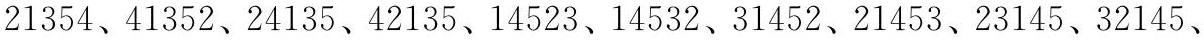
\includegraphics[max width=\textwidth]{2024_10_09_bce9f07034ef55fc9c97g-72} 23415、52341、15234、23514、23541、42351、14235、24513、24531、32451、 13245、34512、34521, 共 41 个; 将上述排列逆过来, 得到至少有 3 个相邻数单调减的排列, 但如 54123 和 32145 均出现过, 这样的既有 3 个数单调增又有 3个数单调减的排列有 $54123 、 53124 、 12543 、 43125 、 52134 、 13542 、 42135$ 、\\
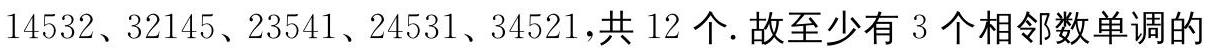
\includegraphics[max width=\textwidth]{2024_10_09_bce9f07034ef55fc9c97g-72(1)}不同排列的数有 $(2 \times(1+8+41)-12=) 88$ 个. 而总的排列数有 $(5!=) 120$个,故符合条件的不同排列有 $(120-88=) 32$ 个.
  \item 先将 3 个蓝球固定, 则 3 个球中间两个位置至少各有 1 个其他球. 若两个位置有 3 个球, 则可以是蓝红黄蓝黄蓝、蓝黄红蓝黄蓝、蓝黄蓝红黄蓝、蓝黄蓝黄红蓝, 共 4 种; 若两端有球, 则中间位置可以是红和黄、黄和红、黄和黄 3 种, 另一个球可以在最前端也可以在最后端, 故共 $(3 \times 2=) 6$ 种. 从而总共有 $(4+6=) 10$ 种不同排列.
  \item 由于每个数均不大于两侧两个数的平均数, 故 5 必在最前面或最后面, 同样, 在余下 4 个数中, 4 必是在剩余 4 个数中最前或最后的, 于是可以一一枚举为: 12345、21345、31245、32145、41235、42135、43125、43215、\\
$51234 、 52134 、 53124 、 53214 、 54123 、 54213 、 54312 、 54321$ ,共 16 个。而这 16 个数中满足条件的只有 $12345 、 41235 、 42135 、 43215 、 51234 、 53124$ 、 53214、54321,共 8 个。
  \item $a_{1}$ 可取 2、3、4 中任一个. 若 $a_{1}=2$, 则 $a_{2}$ 可以取 $1 、 3 、 4$ 中任一个. 如果 $a_{2}=1$ ,那么 $a_{3}=4, a_{4}=3$ ;而如果 $a_{2} \neq 1$ ,那么 $a_{2}$ 可取 3 或 4 ,可能是 $a_{2}=3, a_{3}=4, a_{4}=1$ 或 $a_{2}=4, a_{3}=1, a_{4}=3$ 。故 $a_{1}=2$ 时有 3 种不同排列。而若 $a_{1}=3$ 或 $a_{1}=4$ 时,同理也有 3 种排列,故共有 $(3+3+3=) 9$ 种不同排列。
  \item 公差大于 2 的等差数列有 $\{1,4,7,10\} 、\{2,5,8,11\} 、\{3,6,9$ , $12\}$ 及 $\{1,5,9\} 、\{2,6,10\} 、\{3,7,11\} 、\{4,8,12\}$ 和 $\{1,6,11\} 、\{2,7$ , $12\}$ ,故不同取法数为 $\left(\mathrm{C}_{4}^{3} \times 3+1 \times 6=\right) 18$ 种。
  \item 在方格纸上任取一个边长为 $k$ 的正方形,则它的最左下角的一个方格必属于方格纸的最左下角边长为 $11-k$ 的正方形中。而另一方面,对方格纸中最左下角边长为 $11-k$ 的正方形中任一方格,都可以作一个边长为 $k$ 、最左下角的格子恰为此方格的正方形. 故边长为 $k$ 的正方形共有 $(11-k)^{2}$ 个,因此不同的正方形的取法有 $\left(\sum_{k=1}^{10}(11-k)^{2}=\sum_{k=1}^{10} k^{2}=\right) 385$ 种。
  \item 因为相邻的面涂不同颜色,所以涂同一颜色的两个面只能是对面. 若 4种颜色均涂,则必有 2 种颜色涂对面,另 2 种涂余下的两面,共有 $\mathrm{C}_{4}^{2}$ 种、即 6种不同的涂法。若选取 4 种颜色中的 3 种,则有 $\left(\mathrm{C}_{4}^{3}=\right) 4$ 种选法,对所选 3 种颜色,只可能是对面涂同一种颜色,故只有一种涂法,从而共有 4 种涂法。若取颜色小于 3 种, 则必有两个相邻面颜色相同, 不合要求. 故共有不同涂法 $(4+$ $6=) 10$ 种。
  \item 20 以内有 8 个质因数,依次是 $2 、 3 、 5 、 7 、 11 、 13 、 17 、 19.20$ !的标准分解式中,每个质因数连同它们的指数一起可作为长的因子,也可作为宽的因子,有 2 种选择。 8 个质因数同它们的指数一起共有 $2^{8}$ 种选择,得到 $2^{8}$ 个矩形。由于长与宽可以交换,所以有一半重复,于是共有 $\left(2^{7}=\right) 128$ 个矩形。
  \item $0 . \dot{a} b \dot{c}=\frac{\overline{a b c}}{999}=\frac{\overline{a b c}}{3^{3} \times 37}$. (1)当正整数 $\overline{a b c}=100 a+10 b+c$ 既不是 3的倍数又不是 37 的倍数时, $\frac{\overline{a b c}}{3^{3} \times 37}$ 是最简分数,这样 $\overline{a b c}$ 的个数是 $999-$ $333-27+9=648$ (容斥原理)。(2)当正整数 $\overline{a b c}$ 是 37 的倍数,但不是 3 的倍数时,它的标准分解式中 37 的幂都是 1 ,它与 37 约简后就是(1)中的数。 (3)当正整数 $a b c$ 是 3 的倍数时,(i)如果它的标准分解式中 3 的幂不大于 3 ,那么它与 27 约简后就是(1)中的数;(ii)如果它的标准分解式中 3 的幂大于 3 ,
\end{enumerate}

那么它与 999 约简后就不是 (1)中的数, 这样的数有 $\left(\left[\frac{999}{81}\right]=\right) 12$ 个. 综上所述,化为最简分数后,分子共有 $(648+12=) 660$ 种不同情况。

\section{习 题 2}
\begin{enumerate}
  \item 对每一条边来说, 与它平行的对角线条数 $\leqslant n-2$, 因此与凸 $2 n$ 边形的边平行的对角线不超过 $2 n(n-2)$ 条. 而凸 $2 n$ 边形的对角线的条数是 $\frac{2 n \cdot(2 n-3)}{2}=n(2 n-3)$. 由于 $n(2 n-3)=2 n(n-2)+n$, 由抽屉原则知,必有某条对角线不与该多边形的任何边平行.
  \item 设正方形 $A B C D$ 的边长为 $a$. 当直线 $E F$ 分正方形成两个四边形, 其交点 $E 、 F$ 分别在 $A B 、 C D$ 上, 由于四边形 $A E F D$ 和 $B E F C$ 都是两个直角梯形, 且高为 $a$, 故 $S_{\text {四边形 } A E F D}: S_{\text {四边形 } B E C}=G I: I H$, 这里 $G 、 H$ 分别是 $A D 、 B C$的中点, $G H$ 与 $E F$ 相交于 $I$. 从而 $G I: I H$ 等于 $2: 3$ 或 $3: 2$, 即直线 $E F$ 总经过线段 $G H$ 的分点 $I$, 且点 $I$ 有两个不同位置. 同样地, 当直线 $E F$ 分正方形成两个四边形, 其中点 $E 、 F$ 分别在 $A D 、 B C$ 上时, 直线 $E F$ 总经过线段 $G^{\prime} H^{\prime}$的分点 $I^{\prime}$, 且点 $I^{\prime}$ 亦有两个不同位置, 这里 $G^{\prime} 、 H^{\prime}$ 分别是 $A B 、 C D$ 的中点. 由于 $9=2 \times 4+1$, 结合抽屉原理, 总有三条直线经过同一个分点, 即总有三条直线共点.
  \item 用反证法. 假设点 $P$ 到四个顶点的距离均不小于 17. 连结 $P A 、 P B$ 、 $P C 、 P D$ 。由于 $\angle A P B+\angle B P C+\angle C P D+\angle B P A=360^{\circ}$ ,结合平均数原理 (或抽屉原理)知,上述四个角中总有一个角大于或等于 $90^{\circ}$ ,不妨设 $\angle A P B \geqslant 90^{\circ}$ 。在 $\triangle A P B$ 中, $\angle A P B \geqslant 90^{\circ}$ ,由余弦定理知, $A P^{2}+P B^{2} \leqslant$ $A B^{2} \cdots$ (1), 又 $A P \geqslant 17, P B \geqslant 17$ ,则 $A P^{2}+P B^{2} \geqslant 2 \times 289=578$ ;而 $A B<$ 24 ,则 $A B^{2}<576$ 。利用 (1),有 $576>A B^{2} \geqslant A P^{2}+P B^{2} \geqslant 578$ ,即 $576>578$ ,矛盾!故假设不成立,即结论成立。
  \item 在平面上任取一条直线 $l_{1}$, 并在该直线上取 7 个不同的点, 由于 $7=$ $3 \times 2+1$ ,结合抽屉原理知,至少有四个点是同色的。不妨设四个点 $R_{1} 、 R_{2}$ 、 $R_{3} 、 R_{4}$ 均为红色。再取两条直线 $l_{2} 、 l_{3}$ ,使 $l_{1} / / l_{2} / / l_{3}$ 。过 $R_{i}(i=1,2,3,4)$作 $l_{1}$ 的垂线,交 $l_{2}$ 于 $B_{i}$ ,交 $l_{3}$ 于 $B_{i}^{\prime}$ 。若 $B_{1} 、 B_{2} 、 B_{3} 、 B_{4}$ 中有两个点同为红色或 $B_{1}^{\prime} 、 B_{2}^{\prime} 、 B_{3}^{\prime} 、 B_{4}^{\prime}$ 中有两个点同为红色,那么这两个红点与对应的两个点 $R_{i}$构成同色矩形,结论成立。否则, $B_{i}(i=1,2,3,4)$ 中至少有 3 个点同为蓝色, $B_{i}^{\prime}(i=1,2,3,4)$ 中亦至少有 3 个点同为蓝色, 此时, 由这 6 个蓝色的点中必有 4 个点构成一个同色矩形。
  \item 从这 25 个点中取定一点 $P$, 以点 $P$ 为圆心、 1 为半径作 $\odot P$. 若除去点\\
$P$ 外余下的 24 个点都在圆内,结论成立。不妨设这 25 个点中存在一点 $Q$ ,使 $P Q \geqslant 1$. 以点 $Q$ 为圆心、 1 为半径作 $\odot Q$. 对于这 25 个点除去 $P 、 Q$ 两点外的任意点 $A$, 考察三个点 $P 、 Q 、 A$ ,由于 $P Q \geqslant 1$ ,且这三点中至少有两点距离小于 1, 故 $P A<1$, 或 $Q A<1$, 这说明点 $A$ 在 $\odot P$ 内或在 $\odot Q$ 内. 总之, 这 25 个点要么在 $\odot P$ 内,要么在 $\odot Q$ 内。由抽屉原理,至少有 $\left(\left[\frac{25-1}{2}\right]+1=\right) 13$ 个点在 $\odot P$ 内或在 $\odot Q$ 内.
  \item 设方格纸的中心方格为 $A$ ,则除去 $A$ 外其余 224 个方格可以配成 112对,且每对小方格关于 $A$ 的中心对称。配对小方格中两数之和必不小于 $1+1$ ,即 2 ,且不大于 $56+56$ ,即 112 ,从而配对小方格中两数之和最多有 111 个不同的取值,而现在有 112 对配对小方格,由抽屉原理知,必有两对小方格,其中数字之和相等,而这两对小方格的中心组成以 $A$ 的中心为对称中心的平行四边形,即证明了命题。
  \item 若每个人都写了相同的两个数,则这两个数都出现了 40 次,结论成立。否则有一人写了数 $A$ 和 $B$ ,另一人写了 $B$ 和 $C$ ,对于其他人,要么是 $A$ 和 $B$ ,要么是 $B$ 和 $C$ ,要么是 $A$ 和 $C$ ,总之,每个人写的数必为 $A 、 B 、 C$ 三个中的两个,从而 $A 、 B 、 C$ 三个数共写了 80 次,故由抽屉原理知,至少有一个数至少出现了 $\left(\left[\frac{80}{3}\right]+1=\right) 27$ 次。
  \item 用反证法,即对每一对学生,总存在 1 个(或 1 个以上)问题未解决. 8个学生可组成 $\left(\mathrm{C}_{8}^{2}=\right) 28$ 对,每对学生至少有 1 个问题没有解决。由于 $28=$ $3 \times 8+4$ ,结合抽屉原理,存在 1 个问题,有 4 对学生均未解决,因此至少有 4 个学生不能解出这个问题. 与每个问题被 5 个学生解决矛盾! 假设不成立, 结论成立。
  \item 这 101 个数分别除以 11 ,按所得余数分成 11 类剩余类,分别具有 $11 k, 11 k+1, \cdots, 11 k+10$ 的形式. 若 11 个剩余类中均至少有一个数, 则从这 11 类中分别任取一个数相加,得 $11\left(k_{1}+k_{2}+\cdots+k_{11}\right)+(0+1+2+\cdots+$ $10)=11\left(k_{1}+\cdots+k_{11}\right)+11 \times 5$ ,即这 11 个数之和能被 11 整除。若 11 个剩余类中至少有一类没有上述 101 个正整数中任何一个,由于 $101=10 \times 10+1$ ,结合抽屉原理,必有一个剩余类中至少有 11 个数,取这个剩余类中的 11 个数,有 $11\left(k_{1}+k_{2}+\cdots+k_{11}\right)+11 \cdot r($ 其中 $r=0,1,2, \cdots, 10)$ ,即这 11 个数之和能被 11 整除. 综上两种情况,总能找到 11 个数,它们之和能被 11 整除.
  \item 考虑 $10^{n}$ 个项依次为 $a, a^{2}, a^{3}, \cdots, a^{10^{n}}$ ,并取这 $10^{n}$ 个数对模 $10^{n}$ 的余数. 余数不会出现 0 ,否则 $10 \mid a$ ,这与已知矛盾!因此,仅有( $\left.10^{n}-1\right)$ 个可能的余数,分别为 $1,2, \cdots, 10^{n}-1$ 。由抽屉原理,其中必有两个数 $a^{i} 、 a^{k}(1 \leqslant$\\
$\left.i<k \leqslant 10^{n}\right)$ 的余数相同,因此,其差被 $10^{n}$ 整除,即 $10^{n} \mid a^{k}-a^{i}$ 亦即 $10^{n} \mid$ $a^{i}\left(a^{k-i}-1\right)$ 。因为 $\left(10^{n}, a^{i}\right)=1$ ,故 $10^{n} \mid a^{k-i}-1$ ,即 $a^{k-i}-1=q \cdot 10^{n}$ 。因此, $a^{k-i}=q \cdot 10^{n}+1$ 。这样, $a^{k-i}$ 以 $\underbrace{00 \cdots 01}_{n \text { 个数码 }}$ 结尾。
  \item 设在 $l$ 一侧的 $n$ 个点为 $P_{1}, P_{2}, \cdots, P_{n}$. 考察一切以 $A$ 或 $B$ 为圆心、其上有某个点 $P_{i}$ 的圆,那么每个点 $P_{i}(1 \leqslant i \leqslant n)$ 都是这些以 $A$ 为圆心的圆和以 $B$ 为圆心的圆的交点. 设以 $A$ 和 $B$ 为圆心的圆分别有 $a$ 个和 $b$ 个, 则 $a b \geqslant$ $n$ ,由抽屉原理知,必有 $a \geqslant \sqrt{n}$ 或 $b \geqslant \sqrt{n}$ ,即 $P_{1}, P_{2}, \cdots, P_{n}$ 到 $A 、 B$ 的距离至少有 $\sqrt{n}$ 个不同值。
  \item 将正方形划分为 6 个 $\frac{1}{2} \times \frac{1}{3}$ 的长方形,则由抽屉原理知, 7 个点必有两个点在同一长方形中. 下面只需证明 $\frac{1}{2} \times \frac{1}{3}$ 的长方形中任两点距离不大于 $\frac{\sqrt{13}}{6}$. 设 $A 、 B$ 两点在长方形中, 延长 $A B 、 B A$ 分别交长方形于 $B^{\prime} 、 A^{\prime}$ ,则 $\left|A^{\prime} B^{\prime}\right| \geqslant|A B|$ ,而 $\left|A^{\prime} B^{\prime}\right|$ 为某一直角三角形斜边,而两直角边分别不超过 $\frac{1}{2}$ 和 $\frac{1}{3}$ ,故 $|A B| \leqslant\left|A^{\prime} B^{\prime}\right| \leqslant \sqrt{\left(\frac{1}{2}\right)^{2}+\left(\frac{1}{3}\right)^{2}}=\frac{\sqrt{13}}{6}$ 。
  \item 32 个半径为 1 的圆的总面积为 $32 \times \pi>100$ ,而 $10 \times 10$ 的正方形面积为 100 ,故必有某一点同时属于两个圆,即有两个圆相交。
  \item 若半径为 1 的圆与正方形有公共点, 则必在如图所示的图形中,该图由 1 个 $10 \times 10$ 正方形, 4 个 $2 \times 10$ 的矩形和 4 个半径为 2 的直角扇形组成,故面积为 $10 \times 10+2 \times 10 \times 4+\pi \times 2^{2}=$ $180+4 \pi$ ,而 62 个半径为 1 的圆的面积为 $62 \pi=$ $4 \pi+58 \pi>4 \pi+180$ ,故必有两个圆有交集。
  \item 由于 6 个面积为 1 的图形叠放在面积为 3的区域内,故两两交集之和至少为 $6-3=3$ ,现在\\
(第 14 题)两两的交集区域至多有 $\left(\mathrm{C}_{6}^{2}=\right) 15$ 块,故由抽屉原理,至少有一块不小于 $\frac{3}{15}=\frac{1}{5}$ ,即有两个图形的交集不小于 $\frac{1}{5}$ 。
  \item 由于圆半径为 $\frac{1}{2}$, 故圆心在离正方形边 $\frac{1}{2}$ 的范围内,即在一个 $2 \sqrt{2} \times$ $2 \sqrt{2}$ 的正方形内. 将此正方形划分为 16 个 $\frac{\sqrt{2}}{2} \times \frac{\sqrt{2}}{2}$ 的小正方形,则 17 个圆心中必有两个圆心在同一正方形内,我们已经证明了正方形内两点最大距离即
\end{enumerate}

其对角线的距离,故这两个圆心的距离不大于 $\sqrt{2} \times \frac{\sqrt{2}}{2}=1$ ,所以这两个圆必不外离,即答案是不能放这 17 个圆,使任意两圆都外离.

\section{习 题 3}
\begin{enumerate}
  \item 将 12 个点间隔二染色. 若 6 条弦长度均不同, 那么 6 条弦所对圆心角必分别为 $30^{\circ}, 60^{\circ}, \cdots, 180^{\circ}$, 因此必有 3 条弦的两个端点是异色点, 3 条弦的两个端点是同色点,故两种颜色的点的个数均为奇数个,而事实上,两种颜色点均为 6 个,是偶数个,这就得到矛盾!故不可能 6 条弦长度均不同。
  \item 将正方体八个顶点黑白染色,其中黑点 4 个,白点 4 个,且黑点与黑点,白点与白点间无棱连结。于是,小虫必从白点爬到黑点或从黑点爬到白点,故小虫经过的黑点和白点总次数之差不大于 1 ,而现在两者之差为 $4+3 \times$ $2-4 \times 2=2$ ,故小虫不可能做到。
  \item 分两种情况构造. (1)在 $n(n \geqslant 5)$ 个点中有三点共线. 不妨设点 $A$ 、 $B 、 C$ 共线,且点 $B$ 在线段 $A C$ 上。此时把点 $B$ 染成白色,点 $A$ 和点 $C$ 染成黑色,余下的 $(n-3)$ 个点任意染黑白两色之一。因此,不会有一条直线把白点和黑点分开. (2)在 $n(n \geqslant 5)$ 个点中任意三点不共线,则总有四个点构成一个凸四边形(凸包理论)。不妨设凸四边形 $A B C D$ 。此时把对角顶点 $A$ 和 $C$ 染成白色,点 $B$ 和 $D$ 染成黑色,余下的 $(n-4)$ 个点任意染黑白两色之一。因此,不会有一条直线把白点和黑点分开.
  \item 连接 $2 n$ 个点的 $n$ 条不共端点的线段,且线段两端点异色的不同方法为有限种,则必有一种情况下使所有线段长度之和最小。下证这种情况下任两条线段不相交。事实上,若有 $A_{1} B_{1}$ 和 $A_{2} B_{2}$ 相交,且 $A_{1} 、 A_{2}$ 为红色, $B_{1} 、 B_{2}$ 为蓝色,设交点为 $C$ ,如图,则改成连 $A_{1} B_{2} 、 A_{2} B_{1}$ ,其余线段不变,则由于 $A_{1} B_{2}+A_{2} B_{1} \leqslant\left(A_{1} C+B_{2} C\right)+\left(A_{2} C+B_{1} C\right)=$ $A_{1} B_{1}+A_{2} B_{2}$, 故改动后所有线段和减小了, 这与所设的线段和最小矛盾. 故任两条线段无公共点.
  \item 由于点数 $\geqslant 5$, 且所有点只染两种颜色之一, 由抽屉原理知, 至少有 3个点同色,且构成三角形。从同色三角形的集合中,找一个面积最小的三角形 (由于同色三角形存在且有限,故可作此假设,即利用极端原理)。如果这个三角形的每一条边上都有一个另一种颜色的点,由这三个点构成一个新的同色三角形(颜色异于原三角形)且面积比原三角形小。这与上面选取相违。因此
\end{enumerate}

该三角形至少有一条边上不包含另一种颜色的点.\\
6. 先把每个三角形的最短边染成红色, 剩下的边都染成白色. 由抽屉原理可知, 6 个点 (无三点共线) 所连的 15 条线段双染色必存在同色三角形 (三边同色的三角形). 又每个三角形都有最短边, 则每个三角形都有红色边, 于是上述同色三角形是红色三角形. 在该红色三角形中的最长边也是红色的,即它是另一个三角形的最短边 (由于该边染成红色)。因此有一个三角形的最长边又是另一个三角形的最短边.\\
7. 一方面,总的不同染色法有 $4^{2004}$ 种. 另一方面, 由 $1,2, \cdots, 2004$ 中 10个数组成的等差数列的首项 $a$ 和公差 $d$ 满足 $a \geqslant 1, a+9 d \leqslant 2004$, 所以这种不同的等差数列共有 $\left(\sum_{d=1}^{222}(2004-9 d)=222 \times 2004-9 \times \frac{222 \times 223}{2}=\right)$ 222111 个,故有 10 项同色等差数列的不同染色法种数 $\leqslant 4^{1994} \times 4 \times 222111$.而 $4^{1994} \times 4 \times 222111<4^{2004}$ 种,即至少有一种染色法没有 10 项同色等差数列。\\
8. 记从第 $k$ 个球起共 6 个球为 $T_{k}(1 \leqslant k \leqslant 19)$. 令红球为 1 , 蓝球为 -1 , $T_{k}$ 中 6 个球对应的数之和为 $S_{k}$, 如果有某一个 $k(1 \leqslant k \leqslant 19)$, 使 $S_{k}=0$, 那么 $T_{k}$ 为 3 个红球 3 个蓝球. 若 $S_{1}=0$, 则命题得证. 否则, 不妨设 $S_{1}>0$, 那么由 $S_{1}+S_{7}+S_{13}+S_{19}=0$ 知,必有某个 $S_{i}<0$ 。 设使 $S_{i} \leqslant 0$ 的下标最小的为 $S_{m}$. 由于 $S_{k+1}-S_{k}$ 只能是 $0 、 2 、-2$, 所以 $S_{m-1}$ 必为 2 , 而 $S_{m}$ 必为 0 , 故 $T_{m}$ 是满足条件的 6 个球。\\
9. 由于 1 不在边上, 故从 1 到 $n^{2}$ 这两格之间至多经过 $n-2$ 步(一步即从一格到与它相邻的一格) 可以到达, 而两数之差为 $n^{2}-1$ 且 $n^{2}-1>(n-2)$ $(n+2)$ ,由抽屉原理知,必有一步跨过了 $n+3$ 以上,即必有两个相邻格内之数的差不小于 $n+3$.\\
10. 棋子走遍所有格子一遍回到原来位置共需走 64 步. 将棋盘黑白相间染色, 则横走或坚走都是从一种颜色走到另一种颜色, 而斜着走是走到同一种颜色. 如果棋子从白格走到黑格, 则后面必有黑格走到白格与之对应, 否则不能回到原来的格子,故横走和坚走共走了偶数步。\\
而一共走了 64 步,故斜走必为偶数步。\\
11. 如图给棋盘染色,一个 $2 \times 2$ 的纸片能盖住一个黑格, 一个 $1 \times 4$ 的纸片盖住 0 个或 2 个黑格,由于黑格总数为偶数个,故 $2 \times 2$ 的纸片为偶数个才能覆盖整个棋盘。而现在一张 $2 \times 2$ 纸片换成 $1 \times 4$纸片, 则 $2 \times 2$ 的纸片数为奇数个, 此时必不能覆盖整个棋盘.\\
12. 由于 $n \geqslant 7$ ,故必可找到一个 $4 \times 4$ 的方格,\\
(第 11 题)

使" -1 "落在如图中的阴影方格中。由于开始时阴影格中 8 个数之积为 -1 ,而每次操作中,被变号的阴影格数必为偶数,即 8 个数之积为 -1 不变,故这 8个格子不可能全为" +1 ",从而不能使表格中所有数变为" +1 "。

\begin{center}
\begin{tabular}{|l|l|l|l|l|l|l|}
\hline
0 & 1 & 1 & 0 & 1 & 1 & 0 \\
\hline
1 & 2 & 2 & 1 & 2 & 2 & 1 \\
\hline
1 & 2 & 2 & 1 & 2 & 2 & 1 \\
\hline
0 & 1 & 1 & 0 & 1 & 1 & 0 \\
\hline
1 & 2 & 2 & 1 & 2 & 2 & 1 \\
\hline
1 & 2 & 2 & 1 & 2 & 2 & 1 \\
\hline
0 & 1 & 1 & 0 & 1 & 1 & 0 \\
\hline
\end{tabular}
\end{center}

(第 12 题)\\
(第 13 题)\\
13. 如图把 $7 \times 7$ 个小方格块 $0 、 1 、 2$ 三种颜色染色. $1 \times 1$ 的小块的可能位置只能是标有 0 的块,即四角、中心和边框中间。直接验证可知: $1 \times 1$ 的小块覆盖在染为 0 种颜色的小方格后,另 16 块 $3 \times 1$ 的小块可将整个方格块覆盖。假设 $7 \times 7$ 的方格块中标有 0 的小方块均被 $3 \times 1$ 的矩形小块覆盖。那么九个 $3 \times 1$ 的矩形各盖住 1 个 0 及 2 个 1 ,从而另外七个 $3 \times 1$ 的矩形各盖住 1 个 1 及 2 个 2 ,这样 16 个 $3 \times 1$ 的矩形共盖住了 25 个标有 " 1 "的小方格,而染色的图中总共只有 24 个标有" 1 "的小方格。矛盾!假设不成立,即证明了必有一个标有" 0 "的小方格由 $1 \times 1$ 的小块所盖住。

\section{习 题 4}
\begin{enumerate}
  \item 取 $\triangle A B C$ ,其中 $A B=A C, \angle A=45^{\circ}$ , $\angle A B C=\angle A C B=67.5^{\circ}$ 。过 $C$ 作 $C D \perp A B$ ,在 $D A$上截取 $D E=B D$ 。则 $\triangle A B C$ 分成三个三角形为 $\triangle B C D 、 \triangle C D E 、 \triangle E C A$ 。易知 $\triangle C D E$ 与 $\triangle C E A$ 拼成等腰三角形 $C D A$ ,其中 $\angle A=\angle D C A=45^{\circ}$ ; $\triangle C B D$ 与 $\triangle C D E$ 拼成等腰三角形 $C B E$, 其中 $B C=$ $C E ; \triangle C B D$ 与 $\triangle C E A$ 亦拼成等腰三角形 $C D A$ ,只\\
(第 1 题)须把 $\triangle C B D$ 拼接到 $\triangle C E D$ 的位置即可。所以 $\triangle A B C$ 即为所求的等腰三角形.
  \item 当 $n=2 m+1(m \geqslant 1)$ 时。考虑第 $m+1$ 个方格, 将其中一枚钱币向左搬动一次,于是第 $m$ 个方格中有两枚钱币. 再将第 $m$ 个方格中的钱币向右搬到第 $m+2$ 个方格中,这样依次从右到左,再从左到右,经过 $n-1$ 次搬动,便将钱币都放在最右边的那个方格中,而其余方格中均无钱币. 当 $n=2 m$ 时. 考虑
\end{enumerate}

第 $m$ 个方格, 将其中钱币向右搬动一次, 于是第 $m+1$ 个方格中有两个钱币.再将第 $m+1$ 个方格中的钱币向左搬到第 $m-1$ 个方格中, 这样依次从左到右, 再从右到左, 经过 $n-1$ 次搬动, 便将钱币都放在最右边的那个方格中, 而其余方格中无钱币.\\
3. 考察圆周上相邻数的两两乘积之和 $S$ 的变化情况. 由 $(a-d)(b-c)<0$可得 $a b+c d<a c+b d$. 于是在交换 $b$ 和 $c$ 位置后,和数 $S$ 中只有 3 项受到影响, 且 $a b+b c+c d<a c+c b+b d$, 即交换后使和 $S$ 变大. 但和 $S$ 的取值只有有限个不同的值. 因此, 这样的交换只能进行有限多次.\\
4. 不能. 设 $a 、 b 、 c$ 为任意三个数, 则经过一次操作后得到的三个新数为 $\frac{a+b}{\sqrt{2}} 、 \frac{a-b}{\sqrt{2}} 、 c$. 由于 $\left(\frac{a+b}{\sqrt{2}}\right)^{2}+\left(\frac{a-b}{\sqrt{2}}\right)^{2}+c^{2}=a^{2}+b^{2}+c^{2}$ 。因此,每一次操作都保持三个数的平方和是一个不变量. 已知原来三个数的平方和为 $89^{2}+12^{2}+3^{2}=8074$, 所要达到的三个数的平方和为 $90^{2}+10^{2}+14^{2}=8396$.两个平方和不等, 所以不能达到.\\
5. 不妨设 $m \times n$ 棋盘的行数 $m \leqslant$ 列数 $n$. 第一人总是将车在水平方向移动得尽可能地远, 而使第二个人只能在垂直方向作出反应, 则第一个人可取胜. 事实上, 在第一个人走出 $k$ 步之后, 由第二人作出反应, 那么由于 $m \leqslant n$, 在第二人作过 $k$ 次之后, 第一个人还有作出反应的机会, 因此, 用上述策略, 第一个人必胜.\\
6. 如图, 将正方体的 12 条棱分成四组: $\{A B$, $F G, D H\},\{B C, G H, A E\},\{C D, H E, B F\}$, $\{D A, H F, C G\}$. 不论甲首先涂红的是哪三条棱, 上述四组中总有一组的三条棱尚未涂色, 乙只要把这三条棱涂成绿色, 则正方体的六个面上每个面都会有一条涂绿色的棱, 甲就无法取胜了。所以甲没有必胜的策略。\\
(第 6 题)\\
7. 甲可以采取如下策略:第 1 步先将白子下在左下角的 1 个方格中,然后将其余的方格划分成 $1 \times 2$的矩形小块(如图,右上的一个大方格是 $24 \times 24$ 的方格可分成 $24 \times 12$ 个 $1 \times 2$ 的矩形小块,最左边坚列是 12 个 $2 \times 1$ 的矩形小块,最下边横行是 12 个 $1 \times 2$ 的矩形小块)。以后, 甲每步都将白棋子下在乙所下的矩形小块的另一个小方格中. 显然, 只要乙有地方可以下黑棋子,甲总是可以随之下白棋子。因此,甲有必\\
(第 7 题)

胜策略.\\
8. 甲必获胜. 策略是:甲先挑 $1 、 2^{2001} 、 2^{2002} 、 2^{2003} 、 2^{2004}$ 这 5 个数,则这 5个数变为 $0 、 2^{2001}-1 、 2^{2002}-1 、 2^{2003}-1 、 2^{2004}-1$ ,然后,无论乙挑哪 5 个数,甲都可挑这 5 个数,由于 $2,2^{2}, \cdots, 2^{2000}$ 均为偶数,且 $2+2^{2}+\cdots+2^{2000}<$ $2^{2001}-1$ ,故甲挑选时这 5 个数均大于 0 ,直到乙无法取到 5 个大于 0 的数为止。\\
9. 将第 $n$ 次操作后所得的数组记为 $\left(a_{n}, b_{n}, c_{n}, d_{n}\right)$ 。显然, $a_{n}+b_{n}+c_{n}+$ $d_{n}=0, n=1,2, \cdots$ 。由于 $a_{n}=a_{n-1}-b_{n-1}, b_{n}=b_{n-1}-c_{n-1}, c_{n}=c_{n-1}-d_{n-1}$ , $d_{n}=d_{n-1}-a_{n-1}$, 故 $a_{n}^{2}+b_{n}^{2}+c_{n}^{2}+d_{n}^{2}=2\left(a_{n-1}^{2}+b_{n-1}^{2}+c_{n-1}^{2}+d_{n-1}^{2}\right)-2\left(b_{n-1}+\right.$ $\left.d_{n-1}\right)\left(a_{n-1}+c_{n-1}\right)=2\left(a_{n-1}^{2}+b_{n-1}^{2}+c_{n-1}^{2}+d_{n-1}^{2}\right)+2\left(b_{n-1}+d_{n-1}\right)^{2} \geqslant 2\left(b_{n-1}^{2}+\right.$ $\left.b_{n-1}^{2}+c_{n-1}^{2}+d_{n-1}^{2}\right) \geqslant 2^{2}\left(a_{n-2}^{2}+b_{n-2}^{2}+c_{n-2}^{2}+d_{n-2}^{2}\right) \geqslant \cdots \geqslant 2^{n-1}\left(a_{1}^{2}+b_{1}^{2}+c_{1}^{2}+\right.$ $\left.d_{1}^{2}\right)$. 又因 $a_{1}^{2}+b_{1}^{2}+c_{1}^{2}+d_{1}^{2}>0(a 、 b 、 c 、 d$ 不全相等 $)$ ,所以只要取足够大的 $n_{0}$,可使 $2^{n_{0}-1}\left(a_{1}^{2}+b_{1}^{2}+c_{1}^{2}+d_{1}^{2}\right)>2005^{2} \times 4$ ,即 $a_{n_{0}}^{2}+b_{n_{0}}^{2}+c_{n_{0}}^{2}+d_{n_{0}}^{2}>2005^{2} \times$ 4. 由平均数原理 (或抽屉原理) 知:必有一个数,不妨设 $a_{n_{0}}^{2}>2005^{2}$ ,从而 $\left|a_{n_{0}}\right|>2005$.\\
10. 为方便起见,把五个数的环列写成横列 $v 、 w 、 x 、 y 、 z$ (其中 $v$ 和 $z$ 相邻)。不妨设 $y<0$ ,经变换后得到的环列是 $v 、 w 、 x+y 、-y 、 z+y$ ,变换前后的环列和均为 $x+y+z+w+v>0$ 。现考虑五个整数的平方和再加上每相邻两数和的平方这一整体。那么变换后与前之差是 $\left[v^{2}+w^{2}+(x+y)^{2}+(-y)^{2}+\right.$ $\left.(z+y)^{2}+(v+w)^{2}+(w+x+y)^{2}+x^{2}+z^{2}+(y+z+v)^{2}\right]-\left[v^{2}+w^{2}+x^{2}+\right.$ $\left.y^{2}+z^{2}+(v+w)^{2}+(w+x)^{2}+(x+y)^{2}+(y+z)^{2}+(z+v)^{2}\right]=2 y(v+$ $w+x+y+z)<0$ (这里 $y<0$ 和 $v+w+x+y+z>0$ 都是已知条件)。因此,这一整体(有限的一个正整数)每经过一次变换都至少要减少 2. 而正整数是不能无限减小的,所以该变换必定有终止的时候。\\
11. 设这 $2^{n}$ 个数往右依次为 $a_{1}, a_{2}, \cdots, a_{2^{n}}$ 。我们证明: 经过 $2^{k}$ 次操作后,在 $a_{i}$ 位置上的数为 $a_{i} \cdot a_{i+2^{k}}$ ,这里当下标大于 $2^{n}$ 时,我们认为模 $2^{n}$ 同余的下标则为同一个数。当 $k=1$ 时, 第一次操作后, 第 $i$ 个位置数为 $a_{i} \cdot a_{i+1}$, 第二次操作后,第 $i$ 个位置上数为 $a_{i} \cdot a_{i+1} \cdot a_{i+1} \cdot a_{i+2}=a_{i} \cdot a_{i+2}$ ,即 $k=1$ 时成立;若 $k$ 时成立,即经过 $2^{k}$ 次操作后,第 $i$ 个位置上数为 $a_{i} \cdot a_{i+2}$ ,故再经过 $2^{k}$ 次操作即共 $2^{k+1}$ 次操作后第 $i$ 个数为 $a_{i} \cdot a_{i+2^{k}} \cdot a_{i+2^{k}} \cdot a_{i+2^{k}+2^{k}}=a_{i} \cdot a_{i+2^{k+1}}$ ,故对 $k+1$ 也成立,因此对一切 $k \in \mathbf{N}$ 均成立。于是,经过 $2^{n}$ 次操作后,第 $i$ 个位置上数为 $a_{i} \cdot a_{i+2^{n}}=a_{i}^{2}=+1$ ,即所有数均为 +1 。

\section{习 题 5}
\begin{enumerate}
  \item 若取 $\{51,52,53, \cdots, 100\}$ 共 50 个数,则没有一个数是另一个数的倍
\end{enumerate}

数; 另一方面, 由于每个数可写成 $a \times 2^{t}$ 形式, 这里 $a$ 为奇数, $t$ 为非负整数, 故可将 $1 \sim 100$ 分为 50 个集合 $S_{k}$ ,这里 $S_{k}$ 为 $1 \sim 100$ 中形如 $(2 k-1) \cdot 2^{t}$ 形式的数的集合. 若取 51 个数, 则必有两个数在同一集合中, 而同一 $S_{k}$ 中任两个数必有一个数是另一个数的倍数, 故取 51 个数时, 必有一个数是另一个数的倍数. 综上, 至少取 51 个数才能保证其中必有一个数是另一个数的倍数.\\
2. 设有 $n$ 个砝码, 则可以称出的不同重量至多为 $2^{n}-1$ 个, 这是因为在放砝码一端, 每个砝码有两种选择, 要么放上去, 要么不放上去, 但都不放上去是无法称量的,故至多称不同重量 $2^{n}-1$ 个. 由 $2^{n}-1 \geqslant 2004$, 解得 $n \geqslant 11$.另一方面, 取 11 个砝码为 $1,2,2^{2}, 2^{3}, \cdots, 2^{10}$. 由于 $2004<2^{11}$, 故对任一重量 $k \leqslant 2004, k$ 都可写成二进制 $\left(a_{10} a_{9} \cdots a_{0}\right)_{2}$ 形式,其中 $a_{10}, a_{9}, \cdots, a_{0} \in\{0$, $1\}$, 若 $a_{k}(0 \leqslant k \leqslant 10)=1$, 则取 $2^{k}$ 的砝码置于天平, 由二进制知, 这些砝码的重量和即为欲称的重量, 从而 $1 \sim 2004$ 均可称出来. 故至少要 11 个砝码.\\
3. 最少要交换 10 次才能实现.一方面,首先将第 1 卷与第 2 卷、第 3 卷、第 4 卷、第 5 卷交换位置, 此时第 1 卷调到最右边位置, 即 5 卷书排位为 ( 2 、 $3 、 4 、 5 、 1$ ); 其次将第 2 卷与第 3 卷、第 4 卷、第 5 卷交换位置, 此时第 2 卷调到倒数第 2 位置, 即 5 卷书排位为 $(3 、 4 、 5 、 2 、 1)$ ;再将第 3 卷与第 4 卷、第 5卷交换位置, 得到 5 卷书排位为 $(4 、 5 、 3 、 2 、 1)$ ;最后将第 4 卷与第 5 卷交换位置, 能得到 5 卷书排位为 ( $5 、 4 、 3 、 2 、 1$ ). 因此, 交换 10 次可以满足条件. (这一步是构造.) 另一方面, 证明至少要交换 10 次. 事实上, 将 5 卷书从排位 $(1 、 2 、 3 、 4 、 5)$ 变为 $(5 、 4 、 3 、 2 、 1)$, 任何两卷书 $A$ 和 $B$ 的左右顺序都要改变,而这只有当这两卷书变为相邻时进行交换才能实现。因此,任何两卷书都至少交换 1 次,总共至少交换 $\mathrm{C}_{5}^{2}=10$ 次。(这一步是估计,估计和构造这两步可以交换顺序出现,希从后面的习题中掌握解题要领。)\\
4. 最小值为 9 . 一方面, 如图, 7 个点之间连有 9 条线段满足要求. 事实上, 从 7 个点 $A 、 B 、 C 、 D 、 E 、 F 、 G$ 中任取 3 个点, 要么两点在集合 $\{A, B$, $C\}$ 中, 要么在 $\{D, E, F, G\}$ 中, 而 $A 、 B 、 C$ 中任意两点之间连有线段, $D 、 E 、 F 、 G$ 中任意两点之间亦连有线段. 另一方面, 证明任何满足要求的连线图中至少有 9 条线段. 设 7 个点为 $A 、 B 、 C 、 D 、 E 、 F 、 G$ 。假设 $A$ 与 $B$ 之间无连线,则 $C 、 D 、 E 、 F 、 G$ 五点中每个点都至少与 $A$ 、 $B$ 之一连线, 至少有 5 条线段. 而 $C 、 D 、 E 、 F 、 G$ 五点中共可以组成 $\mathrm{C}_{5}^{3}=10$ 个不同的三点组,每组 3 点之间至少有 1 条线段, 至少共有 10 条线段. 这里可能有重复,但每条线段至多被重复计数 3 次 (如 $C$ 与 $D$ 连线后, 含 $C 、 D$

的三点组有 $\{C, D, E\} 、\{C, D, F\} 、\{C, D, G\}$ 三个), 又 $\frac{10}{3}>3$, 因此, $C 、 D$ 、 $E 、 F 、 G$ 五点中至少有 4 条不同线段 (这 4 条不同线段均异于前面 5 条线段), 从而图中至少有 9 条线段.\\
5. $k$ 的最小值为 $n-2$. 一方面, 证明 $k \geqslant n-2$.从凸 $n$ 边形的某顶点 $A$ 引出 $n-3$ 条对角线, 它们把凸 $n$ 边形分成 $n-2$ 个互不相交的三角形. 由题设, 每个三角形内部至少有一个已知点, 共计至少 $(n-2)$ 个点, 即 $k \geqslant n-2$. 另一方面, 构造一个图放置 $(n-2)$ 个点满足要求. 如图, 取定凸 $n$ 边形 $A_{1} A_{2} \cdots A_{n}$ 的一条边 $A_{1} A_{2}$, 并考察以 $n$ 边形的顶点 $A_{3}, A_{4}, \cdots, A_{n}$, 与边 $A_{1} A_{2}$ 构成的 $(n-2)$ 个三角形. 每个这样的三角形被其他对角线分成若干部\\
(第 $\mathbf{5}$ 题)分, 在包含除去顶点 $A_{1} 、 A_{2}$ 外的第三个顶点的那部分内取一点 (例如 $\triangle A_{1} A_{2} A_{4}$ 中的点的放置是在 $\triangle A_{1} A_{2} A_{4}$ 与 $\triangle A_{3} A_{4} A_{5}$ 的公共部分内部), 共得到 $(n-2)$ 个点. 得到的这 $(n-2)$ 个点满足题中要求. 事实上, 对于任意 $\triangle A_{i} A_{j} A_{k}(1 \leqslant i<j<k \leqslant n)$, 在 3 个角 $\angle A_{1} A_{i} A_{2} 、 \angle A_{1} A_{j} A_{2} 、 \angle A_{1} A_{k} A_{2}$ 中总有 1 个角含于 $\triangle A_{i} A_{i} A_{k}$ 的某个内角中 (如 $\angle A_{1} A_{4} A_{2}$ 含在 $\triangle A_{3} A_{4} A_{5}$ 的 $\angle A_{3} A_{4} A_{5}$ 内), 因此任意 3 个顶点构成的三角形内至少含一个已知点.\\
6. 一方面, 依次按按钮如下: 11123222133313121223113233211, 此时由数字1、2、3 组成的所有三位数 (共 27 个) 在上述序列中各出现一次, 故城堡一定能打开. 另一方面, 由于由 $1 、 2 、 3$ 这 3 个数字所组成的不同的 3 位数共有 27 个, 故只要按出一长串数字序列, 使其中含有全部 27 个 3 位数即可. 该串序列中,除了所按的前两个数字之外,从第 3 个数字开始往后的每 1 个数字都是 1 个三位数的个位数字(如 111232 中含有 4 个三位数:111、112、123、 232). 因此, 为了按出全部 27 个 3 位数, 至少要按 29 次按钮.\\
7. 一方面,取 $A=(1,1,0,0,0), B=(0,0,0,1,1), C=(1,0,1$, $0,1), D=(0,1,1,1,0)$. 直接验证, 有 $d(A, B)=4, d(A, C)=3, d(A$, $D)=3, d(B, C)=3, d(B, D)=3, d(C, D)=4$. 因此, 从集合 $S$ 中能取出 4 个元素, 使它们之中任何两个的距离都大于 2 . 另一方面, 若有 5 个元素,其中任意两个的距离都大于 2 . 又由抽屉原理知, 其中总有 3 个元素的第五个分量相同, 不妨设元素 $A 、 B 、 C$ 的第五个分量都是 0 . 由对称性可设 $A=(0$, $0,0,0,0)$. 因为 $d(A, B)>2, d(A, C)>2$, 所以 $B$ 和 $C$ 的前 4 个分量中都至少有 3 个分量为 1 , 此时 $d(B, C) \leqslant 2$, 矛盾! 综上, 最多可取出 4 个元素使它们两两之间的距离都大于 2 .\\
8. 一方面, 如图 (a)中 9 个方格标记星号, 直接验证知满足条件.\\
(第 8 题)\\
另一方面,对于图(b)中标为黑色的 9 个方格,无论棋盘上的哪个方格中标上星号,都至多与这 9 个黑格中的 1 格有公共边或公共顶点。因此,满足题中的要求,至少要在 9 个方格中标上星号。综上,最少要有 9 个方格标记星号才能满足条件.\\
9. $k$ 的最小值为 9. 一方面,假设 $k \leqslant 8$ ,且这 $k$ 个人中,有 $(k-1)$ 个人互相认识,另外 1 个人不认识前面 $(k-1)$ 个人中任何一个。此时,既不存在 8 个人,将他们两两分成 4 组,每组中的两个人互相认识;也不存在 4 个人,将他们两两分成 2 组,每组中的两个人互相不认识,因此, $k \geqslant 9$ 。另一方面,设有 9 个人 $A_{1}, A_{2}, \cdots, A_{9}$ 。不妨设这 9 人中有 2 人不相识(否则,这 9 个人互相认识,因此存在 8 个人,可将他们两两分成 4 组,每组中的两个人互相认识),即 $A_{8}$ 与 $A_{9}$ 不认识。如果 $A_{1}, A_{2}, \cdots, A_{7}$ 中有两个人不认识,设 $A_{6}$ 与 $A_{7}$ 不认识,那么存在 4 个人,分成两组 $\left\{A_{6}, A_{7}\right\}$ 和 $\left\{A_{8}, A_{9}\right\}$ ,每组中的两个人互相不认识,结论成立。如果 $A_{1}, A_{2}, \cdots, A_{7}$ 中任意两个人均相识。分两种情况:情形(1):若 $A_{8}$ 与 $\left\{A_{1}, \cdots, A_{7}\right\}$ 中某个人 (设为 $A_{1}$ ) 相识, 则 4 组 $\left\{A_{1}, A_{8}\right\} 、\left\{A_{2}, A_{3}\right\}$ 、 $\left\{A_{4}, A_{5}\right\} 、\left\{A_{6}, A_{7}\right\}$ 中每组两个人互相认识,结论成立;同样,若 $A_{9}$ 与 $\left\{A_{1}, \cdots, A_{7}\right\}$ 中某 个人相识,结论亦成立。情形(2):若 $A_{8}$ 和 $A_{9}$ 与 $\left\{A_{1}, \cdots\right.$ , $\left.A_{7}\right\}$ 中所有人都互不认识,那么可选两组 $\left\{A_{8}, A_{1}\right\}$ 和 $\left\{A_{9}, A_{2}\right\}$ ,每组两个人都互不认识,结论亦成立. 总之, 9 个人满足条件。\\
10. 一方面, 设 $A 、 B 、 C$ 是正 $n$ 边形的相邻三个顶点. 考察由点 $B$ 引出的 ( $n-1$ )条线段(边与对角线)及对角线 $A C$ ,由于从 $B$ 引出的 $(n-1)$ 条线段两两有公共点 $B$ ;线段 $A C$ 与从 $B$ 引出的 $(n-1)$ 条线段要么有公共点 $A$ ,要么有公共点 $C$ ,要么有公共点在线段 $A C$ 内。因此,这 $n$ 条线段任意两条线段都有公共点,所以至少需要 $n$ 种不同颜色。另一方面,证明用 $n$ 种不同颜色满足要求。当 $n$ 为奇数,即 $n=2 k+1$ 时,任意一条对角线总与正 $n$ 边形的某条边平行,因此正 $(2 k+1)$ ( $k$ 为正整数)边形的所有边和对角线恰好可分为 $n$ 组平行

线段(每组的代表方向是 $n$ 边形的边); 当 $n$ 为偶数, 类似地正 $n$ 边形的所有边和对角线可分成 $n$ 组平行线段 (每组的代表方向是 $n$ 边形的边和隔一个顶点所连的对角线). 总之, 正 $n$ 边形的所有边和对角线可分成 $n$ 组平行线段, 每组线段涂上同一种颜色, $n$ 种颜色就满足要求. 因此, 满足题中要求的涂色法最少要用 $n$ 种颜色。\\
11. 一方面, 写有 1 的方格共有 4 个邻格, 而整个表中只有两个方格写有 2 , 故在 1 的邻格中一定有至少为 3 的数. 故所有邻格内数差的最大值至少为 2. 另一方面, 图中用粗实线画出十字线将方格表分成 4 个直角形部分. 在左下和右上两部分中依次填写奇数; 在左上和右下两部分中依次填写偶数, 直接验证并观察知, 该填数方法满足条件要求, 即数 $n$ 恰出现 $n$ 次, 且使得任何两个相邻方格中的数的差为 1 或 2 , 故两个相邻两个小格中的数的差的最大值为 2 。\\
(第 11 题)\\
12. 取 $4 k+1$, 其中 $k=0,1, \cdots, 500$ 共 501 个数, 则每两个数差均为 4的倍数, 即为合数, 故可取 501 个数. 而另一方面, 相邻 4 个数中任两数之差必为非合数, 故相邻 4 个数中仅能取 1 个,从而 2004 个数中可取 $\left(2004 \times \frac{1}{4}=\right) 501$ 个数,故至多可取 501 个数.\\
13. 一条直线可将平面分为 2 部分, 设已有 $n$ 条直线, 且分为 $S(n)$ 部分,则添上第 $n+1$ 条直线时, 第 $n+1$ 条直线至多被前 $n$ 条直线分为 $n+1$ 段, 而每 1 段将前面的 1 部分划分成 2 部分, 即增加 1 部分, 所以至多共增加 $n+1$ 部分, 即 $S(n+1) \leqslant S(n)+(n+1)$, 从而 $S(n) \leqslant S(n-1)+n \leqslant S(n-2)+$\\
$n+(n-1) \leqslant \cdots \leqslant n+(n-1)+\cdots+2+S(1)=\frac{1}{2}\left(n^{2}+n+2\right)$ ,即 $n$ 条直线至多将平面划分为 $\frac{1}{2}\left(n^{2}+n+2\right)$ 部分。另一方面,每添上第 $n$ 条直线时,保证与前面的直线不平行,且不过前面直线的交点,则此直线恰分为 $n$ 段,此时有 $S(n)=n+(n-1)+\cdots+2+S(1)=\frac{1}{2}\left(n^{2}+n+2\right)$ 。故最大值为 $\frac{1}{2}\left(n^{2}+\right.$ $n+2$ ).\\
14. 若将棋盘分为 16 个 $2 \times 2$ 的小棋盘, 每个小棋盘染一种颜色,则 16种颜色是满足条件的。若染了 17 种颜色,由于 $\frac{64}{17}<4$ ,则必有某种颜色的格子少于 4 个. 对于某种颜色, 3 个或 3 个以下的格子均不能保证每个格子有两个同色的格子与它有公共边,所以 17 种颜色是不行的. 故最多可染 16 种颜色.\\
15. 设取有 $a_{1}, a_{2}, a_{3}, \cdots, a_{n}$ 共 $n$ 个数,则若 $a_{i}-a_{j}=a_{k}-a_{s}$, 则 $a_{i}+$ $a_{s}=a_{j}+a_{k}$ ,无论 $i$ 是否等于 $s$ 或 $j$ 是否等于 $k$ ,均不满足题意,故不存在 $i 、 j$ 、 $k 、 s$ 使 $a_{i}-a_{j}=a_{k}-a_{s}$ 。不妨设 $a_{1}<a_{2}<\cdots<a_{n}$ ,则 $a_{u}-a_{v}(u-v>0)$ 共有 $\mathrm{C}_{n}^{2}$ 个值,而 $a_{u}-a_{v}$ 最大为 13 ,最小为 1 ,故依题意知, $\mathrm{C}_{n}^{2} \leqslant 13$ ,从而 $n \leqslant 5$ 。另一方面,取 $\{1,4,5,10,12\}$ ,则满足题意。综上,至多可取 5 个数。\\
16. 若该数含有数字 5 ,则尾数为 5 ,从而不能被 $2 、 4 、 6 、 8$ 整除,即该数最多含有 5 个不同数字;若该数不含 5 ,则该数至多有 8 个数字出现,即至多含有 8 个不同数字。另一方面,数 6478319232 能被组成它的数字1、2、3、 $4 、 6 、 7 、 8 、 9$ 整除,故符合要求的数最多含有 8 个不同的数字。\\
17. 一方面,可以作 7 个满足要求的三角形,它们是 $\triangle A_{1} A_{2} A_{3}, \triangle A_{1} A_{4} A_{5}, \triangle A_{1} A_{6} A_{7} ; \triangle A_{2} A_{4} A_{6}$, $\triangle A_{2} A_{5} A_{7} ; \triangle A_{3} A_{4} A_{7}, \triangle A_{3} A_{5} A_{6}$ 。这七个三角形中任意两个至多有一个公共顶点(直接验证可知)。另一方面,假设以 $A_{1}, A_{2}, \cdots, A_{7}$ 为顶点作 8 个三角形,则这些三角形顶点共出现 24 次,对七个点而言,由抽屉原理知,存在一个点至少出现 $\left(\left[\frac{24}{7}\right]+1=\right) 4$ 次。不妨设点 $A_{1}$ 出现在 4 个三角形中。再考察这 4 个三角 (第 17 题)形除 $A_{1}$ 点外的顶点出现的次数是 8 次,对六个点 $A_{2}$ , $A_{3}, \cdots, A_{7}$ 而言,由抽屉原理知,有一个点至少出现 $\left(\left[\frac{8}{6}\right]+1=\right) 2$ 次。不妨设点 $A_{2}$ 至少出现两次,因此存在两个三角形有公共点 $A_{1}$ 和 $A_{2}$ ,与题设相违!因此满足条件的三角形最多可以作 7 个。\\
18. 先考查连续的 11 个正整数,例如从 1 至 11中至多可取出多少个数满足条件。如图排在圆周上的这 11 个数中,任意相邻两数的差的绝对值都为 4 或 7. 故从 $1,2, \cdots, 11$ 中至多取出 5 个满足条件的数 (因为任取 6 个数,则必有两个数在上述圆周上相邻),如 $1,4,6,7,9 , 1 , 2 , 4 , 7 , 10$ 等等。现在从 $1 \sim 2004$ 中取 $11 k+1 、 11 k+2 、 11 k+4 、 11 k+7 、$ $11 k+10(k=0,1, \cdots, 181)$ 和 2003、2004,共计 $(182 \times 5+2=) 912$ 个数,这 912 个数满足题设要求。\\
事实上,该集合中较大的6个数是2004、2003、2001( $11 \times 181+10 )$ 、 1998(11 $\times 181+7) 、 1995(11 \times 181+4) 、 1993(11 \times 181+2)$ 满足题设. 下只须证 $11 k+1,11 k+2,11 k+4,11 k+7,11 k+10(k=0,1, \cdots, 181)$ 中任意两个数的差的绝对值不等于 4 或 7 . 否则,假设 $|(11 n+x)-(11 m+y)|=$ 4 或 7 ,其中 $0 \leqslant m<n \leqslant 181, x, y \in\{1,2,4,7,10\}$ ,易知 $n=m+1$ ,且 $x \neq y$ ,从而有 $|11+x-y|=4$ 或 7 ,故 $|x-y|=4$ 或 7 。矛盾!所以 $k$ 的最大值至少是 912 。另一方面,假设 $k \geqslant 913$ 。除去 2003,2004两个数后, $S$ 中至少还有 911 个数(这些数从 $1,2, \cdots, 2002$ 中取出)。考察下列抽屉: $A_{1}=\{1,2$ , $3, \cdots, 11\}, A_{2}=\{12,13, \cdots, 22\}, \cdots, A_{i+1}=\{11 i+1,11 i+2, \cdots, 11 i+$ $11\}, \cdots, A_{182}=\{1992,1993, \cdots, 2002\}$ 。由抽屉原理知,必有一个抽屉 $A_{i}$ 中有 $\left(\left[\frac{911}{182}\right]+1=\right) 6$ 个数。即连续的 11 个正整数中要选取 6 个数。由开始讨论中得到的结论可知,这 6 个数中必有两个数的差的绝对值等于 4 或 7 ,与题设矛盾!因此, $k \leqslant 912$. 综上, $k$ 的最大值为 912 。\\
19. 如图,可以放 7 个半径为 1 的圆在圆内, 任意两个圆均不相交. 若大圆内有 8 个小圆,下面证明必有两圆相交. 依题意可知, 8 个圆的圆心均在半径为 2 的圆内,将半径为 2 的圆划分为等分的 7 个扇形,依题意知,必有两个点在同一扇形内,若这两个点的距离不小于 2 , 则必有一个点在圆心上. 于是, 若任两点距离不小于 2 , 则其余 7 个点均在圆周上. 将半径为 2 的圆周等分为 6 份,则另 7 点中由抽屉原\\
(第 19 题)理,必有两点在同一弧上。我们不妨在等分圆弧的时候, 6 个等分点与 7 个圆心均不重合,于是在同一段弧上的两个点距离必小于 2 ,即这两个圆相交。综上知,若放 8 个圆,则必有两个圆相交,故最多可放 7 个圆。\\
20. 若取三个顶点和三条边的中点, 则任两点的距离均不小于 1. 如图,取\\
$B A_{1}=C A_{2}=C B_{1}=A B_{2}=A C_{1}=B C_{2}$ ,而 $B A_{1}<$ 1, 则 $\triangle A C_{1} B_{2} 、 \triangle B A_{1} C_{2} 、 \triangle C B_{1} A_{2}$ 中任两点距离均小于 1 。延长 $A_{1} C_{2} 、 C_{1} B_{2} 、 B_{1} A_{2}$ 交于 $A^{\prime} 、 B^{\prime} 、 C^{\prime}$ ,则 $\triangle A^{\prime} B^{\prime} C^{\prime}$ 的边长小于 2 . 若 $O$ 为 $\triangle A B C$ 的中心, $D$ 、 $E 、 F$ 为 $B^{\prime} C^{\prime} 、 C^{\prime} A^{\prime} 、 A^{\prime} B^{\prime}$ 的中点,则 $\triangle A^{\prime} E F$ 、 $\triangle B^{\prime} F D 、 \triangle C^{\prime} D E$ 的边长小于 1 ,因此这些三角形中的任两点距离均小于 1 ;而且 $O A^{\prime}=O B^{\prime}=O C^{\prime}=$ $2 E O$ ,当 $A_{1}$ 和 $A_{2} 、 B_{1}$ 和 $B_{2} 、 C_{1}$ 和 $C_{2}$ 分别重合时 $O E=\frac{\sqrt{3}}{6}<\frac{1}{3}$ ,故 $O A^{\prime} 、 O B^{\prime} 、 O C^{\prime}$ 在 $\left|A_{1} A_{2}\right|$ 、 $\left|B_{1} B_{2}\right| 、\left|C_{1} C_{2}\right|$ 适当小时,可以小于 $\frac{2}{3}$ ,因此五边形 $O E A_{1} A_{2} F$ 、 $O F B_{1} B_{2} D 、 O D C_{1} C_{2} E$ 中任两点距离均小于 1 。现在 $\triangle A B C$ 被分成 6 个区域(3个三角形和 3 个五边形),由抽屉原理知,若有 7 个点在三角形中,必有两个点在同一区域,则必有两点距离小于1。故至多可以有 6 个点在三角形中,使任两点距离不小于 1.


\end{document}